\documentclass{elsarticle}

\usepackage{graphicx}

\usepackage{oubraces}
\usepackage{epstopdf}

\usepackage{amssymb,amsmath}
%\usepackage{amsthm}
\usepackage{url}
\usepackage{psfrag}
\usepackage{color}
\usepackage{hyperref}
\usepackage{breakurl}
%\usepackage[dvips]{graphics,graphicx}
%\usepackage[dvips]{graphicx}
\usepackage{rotating}

\usepackage{verbatimbox}
\usepackage{epsfig}
\usepackage{chngpage}
\usepackage[title]{appendix}

\usepackage{amssymb}
\journal{Science of Computer Programming}

\newcommand{\paral}{\; \vert \;}
\newcommand{\myvec}[1]{\overrightarrow{#1}}
\newcommand{\Defeq}{\stackrel{\mathrm{df}}{=}}
\newcommand{\Bnfeq}{::=}
\newcommand{\Co}[1]{\overline{#1}}

%
\newcommand{\Bsep}{\: \mid \: }
\newcommand{\Rule}[2]{\displaystyle{\frac{#1}{#2}}}
\newcommand{\SF}[1]{\mathsf{#1}}
\newcommand{\Act}{\mathsf{Act}}
\newcommand{\Vis}{\mathsf{Vis}}
\newcommand{\ActK}{\mathsf{ActK}}
\newcommand{\Proc}{\mathsf{Proc}}
\newcommand{\Procc}{\mathsf{ProcC}}
\newcommand{\Var}{\mathsf{Var}}
\newcommand{\Pred}{\mathsf{Pred}}
\newcommand{\Std}{\mathsf{Std}}
\newcommand{\rms}{\mathrm{S}}
\newcommand{\rmrec}{\mathrm{rec}}
\newcommand{\rmreck}{\mathrm{reck}}
\newcommand{\rmreckR}{\mathrm{reckR}}
\newcommand{\rma}{\mathrm{A}}
\newcommand{\rmp}{\mathrm{P}}
\newcommand{\rmf}{\mathrm{F}}
\newcommand{\rmr}{\mathrm{R}}
\newcommand{\rmfr}{\mathrm{FR}}
\newcommand{\equivS}{\equiv_{\mathrm{S}}}
\newcommand{\SigSA}{\Sigma_{\mathrm{SA}}}
\newcommand{\ltran}[1]{\stackrel{#1}{\longrightarrow}}
\newcommand{\tran}[1]{\stackrel{#1}{\rightarrow}}
\newcommand{\Tran}[1]{\stackrel{#1}{\Rightarrow}}
\newcommand{\nottran}[1]{\stackrel{#1}{\not\rightarrow}}
\newcommand{\Rtran}[1]{\stackrel{#1}{\rightsquigarrow}}
\newcommand{\notRtran}[1]{\stackrel{#1}{\not\rightsquigarrow}}
\newcommand{\trans}[1]{\stackrel{#1}{\rightarrow}_{\mathrm{S}}}
\newcommand{\Par}{\mid}
\newcommand{\restrict}[1]{\!\setminus\!#1}

\newcommand{\mA}{\mathcal{A}}
\newcommand{\mSA}{\mathcal{SA}}
\newcommand{\mWA}{\mathcal{WA}}
\newcommand{\mAK}{\mathcal{AK}}
\newcommand{\aAK}{\mathcal{(A)K}}
\newcommand{\umAK}{\underline{\mathcal{A}}\mathcal{K}}
\newcommand{\un}[1]{\underline {#1}}
\newcommand{\PI}{\mathcal{PI}}
\newcommand{\rom}[1]{\mbox{\rm{#1}}}

\newcommand{\Nil}{\mathbf{0}}
\newcommand{\New}[1]{\nu#1\: }
\newcommand{\Str}{\equiv}
\newcommand{\stdpred}{\mathsf{std}}
\newcommand{\std}[1]{\mathsf{std}(#1)}
%
\newcommand{\Bch}[2]{\mathsf{before}_{#1}(#2)}

\newcommand{\keys}[1]{\mathsf{keys}(#1)}
\newcommand{\kkey}[1]{\mathsf{k}(#1)}
\newcommand{\key}[1]{[#1]}
\newcommand{\Keys}{\mathcal{K}}
\newcommand{\freshpred}[1]{\mathsf{fsh}[#1]}
\newcommand{\fresh}[2]{\mathsf{fsh}[#1](#2)}

\newcommand{\ta}[1]{\mathsf{ta}(#1)}
\newcommand{\action}[1]{\mathsf{act}(#1)}

\newcommand{\intr}{\mbox{\ $\hat{}$\ }}
%\newcommand{\intr}{\mbox{\; $\widehat{}$\;}}
\newcommand{\sterm}{\mathsf{trm}}
\newcommand{\Sterm}[1]{\sterm(#1)}
\newcommand{\und}[1]{\underline{#1}}
\newcommand{\sqc}{\mathop{\cdot}}
\newcommand{\card}[1]{|#1|}
\newcommand{\bydef}{\stackrel{\emph{def}}{=}}
%
\newcommand{\Angle}[1]{\langle #1 \rangle}
\newcommand{\Tri}{\triangleright}
\newcommand{\Hole}{\bullet}
\newcommand{\rec}[1]{\mathrm{rec}\, #1}
\newcommand{\Rec}[1]{\rec #1 .}
\newcommand{\Rch}{\mathsf{Rch}}
\newcommand{\prune}{\pi}
\newcommand{\Prune}[1]{\prune(#1)}
\newcommand{\Root}[1]{\mathsf{rt}(#1)}
\newcommand{\hole}{\mbox{$[\ ]$}}

\newcommand{\Bis}{\sim}
\newcommand{\Biss}{\Bis_{\mathsf{S}}}
\newcommand{\Bisf}{\Bis_{\mathsf{F}}}
\newcommand{\Bisfr}{\Bis_{\mathsf{FR}}}
%\newcommand{\Bisu}{\Bis_{\Un}}
\newcommand{\Sim}{\mathcal{S}}
\newcommand{\Rem}{\backslash}
\newcommand{\sqeqt}{\sim}
% rules:
% static rule
\newcommand{\one}{\mbox{(I)}}
\newcommand{\onef}{\mbox{(1)}}
\newcommand{\oner}{\mbox{(1R)}}
% choice rule
\newcommand{\two}{\mbox{(II)}}
\newcommand{\twof}{\mbox{(2)}}
\newcommand{\twor}{\mbox{(2R)}}
% choice axiom
\newcommand{\thr}{\mbox{(III)}}
\newcommand{\thrf}{\mbox{(3)}}
\newcommand{\thrr}{\mbox{(3R)}}
\newcommand{\thrpf}{\mbox{(3\,$'$\!)}}
\newcommand{\thrpr}{\mbox{(3\,$'$\!R)}}
%
%
\newcommand{\Draft}[1]{}
\newcommand{\Comment}[1]{}
\newcommand{\Rev}[1]{{#1}^{-1}}
%\newcommand{\Stefan}[1]{{\bf S$<$} #1 {\bf $>$S}}
\newcommand{\Stefan}[1]{{\bf S(} #1 {\bf )S}}
\newcommand{\rulename}[1]{\textsf{#1}}

\newtheorem{definition}{Definition}
\newtheorem{example}{Example}
\newtheorem{proposition}{Proposition}
\newtheorem{thm}{Theorem}
\newtheorem{lem}[thm]{Lemma}
\newdefinition{rmk}{Remark}
\newproof{pf}{Proof}
\newproof{pot}{Proof of Theorem \ref{thm2}}


\usepackage{hyperref}

\makeatletter
\providecommand{\doi}[1]{%
  \begingroup
    \let\bibinfo\@secondoftwo
    \urlstyle{rm}%
    \href{http://dx.doi.org/#1}{%
      doi:\discretionary{}{}{}%
      \nolinkurl{#1}%
    }%
  \endgroup
}
\makeatother

\begin{document}

\begin{frontmatter}


\title{Local reversibility in a Calculus of Covalent Bonding}

\author{Stefan Kuhn, Irek Ulidowski}

\address{Department of Informatics, University of Leicester, Leicester, LE1 7RH, United Kingdom}

\begin{abstract}
We introduce a process calculus with a new prefixing operator that allows us to model 
locally controlled reversibility. 
Actions can be undone spontaneously, as in other reversible process calculi, or as pairs of concerted 
actions, where performing a weak action forces undoing of another action. The new operator in its 
full generality allows us to model out-of-causal order computation, where causes are undone 
before their effects are undone, which goes beyond what typical reversible calculi can express. 
However, the core calculus, which uses only the reduced form of the new operator, is well behaved as it 
satisfied causal consistency.
We demonstrate the usefulness of the calculus by modelling the hydration of formaldehyde in water 
into methanediol, an industrially important reaction, where the creation and breaking of some 
bonds are examples of locally controlled out-of-causal order computation.
\end{abstract}

\begin{keyword}
Reversible process calculi \sep local reversibility \sep modelling of biochemical reactions
\end{keyword}

\end{frontmatter}

%% main text
\section{Introduction}\label{sec:intro}
There are many different computation tasks which involve undoing of previously 
performed steps or actions. Consider a computation where the action $a$ causes the action $b$,
written $a<b$, and where the action $c$ occurs independently of $a$ and $b$.
There are three  executions of this computation that preserve \emph{causality},
namely $abc$, $acb$ and $cab$. We note that $a$ always comes before $b$.
There are several conceptually different ways of undoing these actions
\cite{irek2014}. {\em Backtracking}
is undoing in precisely the reverse order in which they happened. So, undo $b$ undo $c$ undo
$a$ is a backtrack of the execution $acb$.
{\em Reversing\/} is a more general form of undoing: here actions can be undone in any
order provided causality is preserved (meaning that causes cannot be undone before effects).
For example, undo $c$ undo $b$ undo $a$ is a reversal of $acb$ for the events $a,b$ 
and $c$ above.


There are networks of reactions in biochemistry, however, 
where actions are undone seemingly \emph{out-of-causal order}.
The creation and breaking of molecular bonds between the proteins involved
in the ERK signalling pathway is a good example 
of this phenomenon ~\cite{Irek2012}. Let us assume for simplicity that the creation of molecular 
bonds is represented by actions $a,b,c$ where, as above, $a<b$ and $c$ is independent 
of $a$ and $b$. In the ERK pathway, the molecular bonds are broken in the following 
order: undo $a$, undo $b$, undo $c$, which seems to undo the cause $a$ before the effect $b$. 

We introduced informally a novel and purely local in character mechanism for undoing
of computation in short papers \cite{merevcomp2015,KU16}. Here, we build a process calculus 
around this mechanism and give it operational semantics.
We then discuss various properties that hold in the calculus. Most importantly, 
we show that out-of-causal order computation can be modelled in the calculus. Hence, in general,
the \emph{causal consistency} property \cite{danos2004ccsr} does not hold. There are reachable states 
that can only be arrived at by a mixture of forward and reverse steps. However, we argue that 
causal consistency holds in a restricted version of our calculus, thus the full calculus is in effect
a ``conceptual'' extension of a causally consistent reversible process calculus. The benefits
of the calculus are shown by modelling hydration of formaldehyde 
in water. The molecules of formaldehyde and water are modelled as compositions 
of carbon, oxygen and hydrogen atoms. When composed in parallel, the molecules react 
and the reactions are represented by sequences of transitions of \emph{concerted actions}. 
We are able to represent different forms of reversibility, including out-of-causal order 
reversibility, and computation can proceed in any directions without external control.

The novel features of our calculus are introduced via an example of a simple catalytic reaction.
Consider two molecules $A$ and $B$ that are only able to bond if assisted by a catalyst $C$. 
Once $A$ and $B$ are bonded with the catalyst $C$, $A$ bonds with $B$ and, at the same time, 
the bond between $A$ and $C$ is broken. Finally, the bond between $B$ and $C$ is broken. 
This is illustrated below.
% The reaction steps are shown in Figure~\ref{fig:intro}.

\begin{figure}[h!]
\psfrag{A}{$A$}
\psfrag{B}{$B$}
\psfrag{C}{$C$}
\psfrag{c}{$c$}
\psfrag{d}{$d$}
\psfrag{q}{$q$}

  \centering
    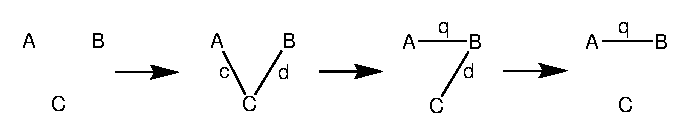
\includegraphics[width=0.8\textwidth]{exampleintro}
  \caption{A catalytic reaction.}
  \label{fig:intro}
\end{figure}

We assume $A  \bydef  (a;p).A'$, $B  \bydef  (b,p).B'$ and $C \bydef  (a,b).C'$, where
$A',B'$ and $C'$ represent further potential behaviour of the molecules $A,B$ and $C$.
%\Stefan{Note that we write the process name with a $'$ instead of $\Nil$ for easy identification of 
%processes without implying any semantical change.} 
We use a new prefix operator $(s;p).P$ where $s$ is a sequence of actions or executed
actions and $p$ is a \emph{weak} action. Initially the actions in $s$ take place, and then $p$ takes place.
%and then we compute with $P$.  
The molecules $A,B$ and $C$ can bond by performing synchronously the
matching actions according to the communication function $\gamma(a,a)=c$, $\gamma(b,b)=d$ and
$\gamma(p,p)=q$, producing thus new actions $c,d$ and $q$ respectively. A weak action $p$ can be left out
in $(s;p)$ 
resulting in the simple prefix $(s).P$ (as in $B$ and $C$ above).
In general, the actions of $s$ in $(s;p).P$ can take place in any order, very much like in
\cite{Danos2007ccsr,Irek2012}, and the new feature is that $p$ can happen only if
all actions in $s$ have already taken place. Once $p$ takes place, one of the executed
actions in $s$ must be undone immediately: this is our new mechanism for
triggering reverse computation.  We shall model these two almost simultaneous
events as a transition of concerted actions. This is a realistic representation of the mechanism 
of covalent bonding, 
the most common type of chemical bonding between atoms, hence we call our calculus
a \emph{Calculus of Covalent Bonding}.

Returning to our example, we represent the system of molecules $A,B$ and $C$ as 
$((a;p).A' \paral (b,p).B' \paral (a,b).C') \setminus \{a,b,p\}$, 
where `$\paral$' is the parallel composition and `$\setminus$' the restriction as in
ACP \cite{BaetenBook}.
We note that $A$ and $B$ cannot interact initially since $\gamma(a,b)$ is not defined. 
They can however both 
interact with $C$:
\begin{flalign*}
&(a;p).A' \paral (b,p).B' \paral (a,b).C' \xrightarrow{c[1]} (a[1];p).A' \paral (b,p).B' 
	\paral (a[1],b).C' \xrightarrow{d[2]} \\
&(a[1];p).A' \paral (b[2],p).B' \paral (a[1],b[2]).C'
\end{flalign*}
Numbers 1 and 2 are the \emph{communication keys} \cite{PhillipsUlidowski06,Irek2007}: they indicate 
which pairs of actions have bonded. 
Molecules $A$ and $B$ can now bond on $p$ (with the key 3), producing the action $q[3]$. 
This causes immediately the breaking of the bond $c[1]$, which means undoing of 
the action $a$ in $A$ and action $a$ in $C$ (and still leaving $A$ and $B$ bonded). 
We model such an event of creating a bond and simultaneously breaking another bond by a
pair of \emph{concerted actions}:
\begin{flalign*}
	&(a[1];p).A' \paral (b[2],p).B' \paral (a[1],b[2]).C' \xrightarrow{\{q[3],\underline{c}[1]\}}\\
       &  (a;p[3]).A' \paral (b[2],p[3]).B' \paral (a,b[2]).C'
\end{flalign*}
The bond with the key 3 on the weak action $p$ in $A$ is unstable, and thus gets \emph{promoted} to 
a stable and stronger 
bond on $a$ and $p$, which is modelled by the following rewrite:
\begin{flalign*}
&(a;p[3]).A' \paral (b[2],p[3]).B' \paral (a,b[2]).C' \Rightarrow (a[3];p).A' \paral (b[2],p[3]).B' 	\paral (a,b[2]).C'
\end{flalign*}
Finally, the catalyst dissolves the bond with $B$:
\begin{flalign*}
(a[3];p).A' \paral (b[2],p[3]).B' \paral (a,b[2]).C'
\xrightarrow{\underline{d}[2]} (a[3];p).A' \paral (b,p[3]).B' \paral (a,b).C'
\end{flalign*}
We note that $A$ and $B$ are now bonded although the synchronisation function did not allow 
it to happen initially. The main consequence of this is that the bond between $a[3]$ and $p[3]$ is 
\emph{irreversible}, namely it cannot be undone.
Looking at the pattern of doing and undoing of bonds we obtain $c[1] d[2] 
q[3] \underline{c}[1] \underline{d}[2]$. Since creation of bonds $c$ and $d$ causes the bond $q$, 
we have here an example of an out-of-causal order computation.

The calculus CCB is given \emph{Structural Operational Semantics} (SOS for short)
style semantics. This includes
novel SOS rules for concerted actions and three rewrite rules that prescribe when bonds on weak actions 
can be promoted to strong action bonds. We show that CCB is a well behaved calculus by proving
a number of useful properties. For example, the sub-calculus with the simple prefixing operator
$(s).P$ satisfies causal consistency. We show that the full calculus allows us to represent 
out-of-causal order computation patterns via the hydration of formaldehyde in water case study. 

Next we summarise the main items of related work.

\subsection{Related Work}

Scientists started to investigate the speed of chemical reactions and the rates achieved as soon as 
the concept of chemical reactions was first developed. The behaviour of a system of compounds over 
time can be modelled using a set of ordinary differential equations (ODEs). The fast calculations 
of such ODEs were popularised by Gillespie \cite{Gillespie} in order to show the dynamic behaviour 
of systems of chemical compounds. When biochemical processes, which involve not only small molecules 
but also macromolecules, cells and membranes, were modelled attention turned to how
the individual objects were represented and how they behaved, and the usefulness of computer 
science methods was demonstrated in \cite{fontana}.

Process calculi are very successful formalisms for representing concurrent and distributed
systems. Each component of a system has its definition which specifies what it does and how it 
interacts with other components. The behaviour of the system emerges then from the independent
actions of the components and from the interactions between them.
Calculus of Communicating Systems (CCS) \cite{Milner1980}, Communicating Sequential Processes (CSP) 
\cite{HoareBook}, and the $\pi$-calculus \cite{MilnerPi} are examples of process calculi.
Starting with Regev et al. \cite{regev2001a,regev2001b,regev2004} process calculi, specifically 
the $\pi$-calculus, were used to model biochemical systems. The biochemical compounds  
are represented as processes, and how they react is modelled by communication on ports. A creation
of a bond or a dissolution of a bond is represented as establishing or breaking of a communication
between ports. 
So there is a natural analogy between concurrent processes and biochemical entities in natural 
systems, and between communication among processes and reactions between biochemical entities.
The aim of this work, as stated in \cite{regev2001b}, was to represent suitably biological knowledge in 
processes and to enable computer-based analysis of this representation. This approach was extended
shortly afterwards to include reaction rates \cite{PriameRegev} using the stochastic $\pi$-calculus, 
which was introduced previously in \cite{PriamiStochasticPi}.

Various other calculi, including  Bio-PEPA (\cite{CiocchettaBiopepa}), the biochemical abstract 
machine (BIOCHAM, \cite{biocham}), P systems (\cite{psystems}), BioAmbients (\cite{RegevBioambients}), 
the kappa calculus (\cite{danos2004kappa}) and Brane Calculus (\cite{CardelliBraneCalculi}),
followed aiming to capture various other aspects of biological systems such as,
for example, compartments and  membranes.

Most of biochemical reactions are reversible, and creating bonds is as important in biochemical processes
as breaking of bonds. Hence, it became useful to be able to represent directly reversibility in
process calculi. This realisation lead to the development of a number of reversible
process calculi \cite{danos2004ccsr,Danos2007ccsr,PhillipsUlidowski06,Irek2007,LaneseMS10,Lanese_controllingreversibility,Lanese_controlled,CKV13}, which have application far beyond biochemistry.
Out-of-causal order reversibility, an important aspect of biochemical system which is
typically not captured in traditional reversible process calculi, was first proposed 
in \cite{Irek2012}, where the calculus CCSK 
\cite{Irek2007} is extended with an \emph{execution control mechanism} for 
managing the pattern and the direction of computation. The control mechanism for reversibility
is external to the processes it controls, and it can have a global scope. The calculus introduced 
in this paper has in contrast  no global control and the behaviour
of a biochemical systems emerges from the behaviour of its components. Out-of-causal order computation
was also studied in \cite{Irek2013,irekconcur2013}.

\section{A Calculus of Covalent Bonding}\label{sec:calculus}

In this section we define the calculus introduced informally in the Introduction. 
First, we introduce some preliminary notions and notations.

Let $\mA$ be the set of (forward) action labels, 
ranged over by $a,b,c,d,e,f$. We partition $\mA$ into the set of \emph{strong actions}, written as
$\mSA$, and the set of \emph{weak actions}, written as $\mWA$. Reverse (or past) action labels are members of
$\underline\mA$, with typical members $\un{a},\un b, \un c,\un d, \un e ,\un f$, and represent 
undoing of actions. The set $\mathcal{P}(\mA \cup \underline\mA)$ is ranged over by $L$.

Let $\Keys$ be an infinite set of {\em communication keys} (or {\em keys} for short)
\cite{PhillipsUlidowski06,Irek2007}, ranged over by $k,l, m,n$. The Cartesian product $\mathcal A \times \Keys$, denoted by $\mAK$,
 represents past actions, which are written as $a[k]$ for $a\in \mA$ and $k\in\Keys$. 
Correspondingly, we have the set $\umAK$ that represents undoing of past actions. We use $\alpha, \beta$ to identify actions which are either from $\mA$ or $\mAK$. It would be 
useful to consider sequences of actions or past actions, namely the elements of $(\mA \cup \mAK)^*$, 
which are ranged over by $s,s'$ and sequences of purely past actions, namely the elements of $\mAK^*$, 
which are ranged over by $t,t'$. The empty sequence is denoted by $\epsilon$. We use the notation $\alpha, s$ and
$s,s'$ to denote a concatenation of elements, which can be strings or single actions.

We shall also use two sets of auxiliary action labels, namely the set $(\mA) =\{ (a)\ \mid a\in\mA\}$, and its product with the set of keys, namely $(\mA)\Keys$. These labels will be used in the auxiliary rules when defining
the semantics of CCB.

We now define the Calculus of Covalent Bonding, or CCB for short. The syntax of CCB is given 
below where $P$ is a process term:

$$P ::=  S \ \mid \ (s;b).P \ \mid \ P\paral Q \ \mid \ P\restrict L $$

The set of process identifiers (constants) $\PI$ contains typical elements $S$ and $T$. 
A process identifier $S$ has normally a defining equation $S\bydef P$ where $P$ contains only forward 
actions (and no past actions). There is also a special identifier
 $\Nil$, denoting the deadlocked process, which has no defining equation.

We have a general prefixing operator
$(s;b).P$, where $s$ is a non-empty sequence of actions or past actions. This operator
extends the prefixing operator in \cite{Irek2012}. The action $b$ is a weak action
and it can be omitted, in which case the prefixing is written as $(s).P$ and is called the
\emph{simple prefix}. The simple prefix is the prefixing operator in \cite{Irek2012}. 
One of the actions in $s$ in $(s).P$ may be a weak action from $\mWA$. If $s$ is a sequence that contains   
a single action, then the action is a strong action and the operator 
is the prefixing operator of CCS \cite{Milner1980}.
We omit trailing $\Nil$s so, for example, $(s).\Nil$ is written as $(s)$.
%
% Move this example to somewhere later
%
\Comment{\Stefan{We will only use cases in this paper where processes are of the form $(s).\Nil$. We still have the possibility of 
processes like $(s).(s').\Nil$ in our calculus. This could be used to model protein functions in biological systems, for example 
base excision repair (\cite{Köhler2014}. For this a protein ``walks'' along a strand of DNA and repairs faults which occurred in 
DNA replication. Such a protein could be modelled by having the walk modelled in $s$ and the repair mechanism in $s'$, combining them to a model like $(s).(s').\Nil$.}
}
%
%
The new feature of the operator $(s;b).P$ is the execution of the weak action $b$, which
can happen only after all the actions in $s$ have taken place. Performing $b$ then forces
undoing one of the past actions in $s$ (by the \rulename{concert} rule in Figure~\ref{fig:csos}).

$P\paral Q$ represents two systems $P$ and $Q$ which can perform actions or reverse actions on
their own, or which can interact with each other according to a communication function
$\gamma$. As in the calculus ACP \cite{ACPBook}, the communication function is a partial function 
$\gamma: \mathcal A \times \mathcal A \rightarrow \mathcal A$ which is commutative and associative. The function
$\gamma$ is used in the operational semantics to define when two processes can interact. Processes 
$P$ and $Q$ in $P\paral Q$ can also perform a pair of concerted actions,
which is the new feature of our calculus.  We also have the ACP-like restriction operator 
$\setminus L$, where $L$ is a set of labels. It prevents actions from taking place and, due to 
the synchronisation algebra used, it also blocks communication. If $\gamma(a,b)=c$ then $a.P$ and $b.Q$
cannot communicate in $(a.P\paral b.Q)\setminus c$.
Note that we do not use here the usual relabelling 
operator $[f]$, where $f: \mA \rightarrow \mA$, which could be easily added.

%
%move this elsewhere?
%
The example in the Introduction and our main example in Section~\ref{sec:bigexample} seem to indicate that only
simple processes of the form $(s;b).\Nil$ are sufficient in the modelling of chemical reactions. 
However, there are examples where a nested prefix $(s;b).(s';b').P$ is useful. 
Consider a base excision repair as in \cite{Köhler2014} where a protein ``walks'' along 
a strand of DNA and repairs faults which occurred in the DNA replication. The walking along a DNA strand 
could be modelled by actions in $s$, and, once a fault is found, the repair mechanism could be modelled
by the actions in $s'$. Another example where the full calculus is useful is a model of long 
standing transactions with compensations in \cite{Irek2012}.


The set of \emph{process terms} is ranged over by $P,Q$ and $R$ and is denoted by $\Proc$. 
In the setting of CCB these terms are called simply \emph{processes}. 
A context $C\hole$ is a process term containing a \emph{hole}, represented by $\hole$. 
Formally, contexts are defined by
the following syntax: $C::= \hole \mid (s;b).C \mid P\paral C \mid C \paral P \mid C\restrict L $.
The term $C[Q]$ denotes the result of filling the hole in the context $C\hole$ with the process $Q$.
We say that $R$ is a \emph{subprocess} of $P$ if $P$ is $C[R]$ for some context $C\hole$.

We define the semantics of our calculus by a labelled transition system,
LTS for short, which is a structure $(St,AL,\rightarrow: \subseteq St \times AL \times St)$
with $St$ the set of states, $AL$ the set of action labels and $\rightarrow: 
\subseteq St \times AL \times St$ the labelled transition relation.
The set of states $St$ is the set $\Proc$. In practice, all our results and examples hold for
\emph{consistent} processes, namely processes
reachable from standard processes (see Definition~\ref{consistent}). 
The action labels are the forward actions $\mAK$, 
the reverse actions $\umAK$ and the \emph{pairs of concerted actions} $\mAK \times \umAK$. 
%
The labelled transition relation is defined by SOS rules (Figures~\ref{fig:fsos}--\ref{fig:sc}) 
and rewrite rules (Figure~\ref{fig:reduction}), where
the rules in Figures~\ref{fig:fsos}--\ref{fig:reversesos}
are influenced by \cite{Irek2007}. 
Note that
sequences $s$ and $t$ are members of $(\mathcal{A}\cup\mathcal{AK})^*$ and $\mathcal{AK}^*$
respectively in Figures~\ref{fig:fsos}--\ref{fig:csos}.

We now introduce and explain the SOS rules before returning to 
the rewrite rules. Let $r$ be an SOS rule for an operator $f$ of CCB as in 
Figures~\ref{fig:fsos}--\ref{fig:csos}. 
%Then, $f$ is the operator of $r$ and the elements of $X$ are the arguments of $r$. 
%We write $rules(f)$ for the set of SOS rules for $f$. 
Transitions above the horizontal bar in $r$ are called \emph{premises}. 
The set of premises is written as
$pre(r)$. The transition below the bar in $r$ is the $\emph{conclusion}$ and 
is written as $con(r)$. 
%
\begin{figure}[t] 
\[
\begin{array}{ll}
\Rule
{}
{\std{\Nil}}
\qquad &
\Rule
{}
{\fresh{m}{\Nil}}
\\[15pt]
\Rule
{\std{P}}
{\std{S}}
\quad
S \bydef P
\qquad &
\Rule
{\fresh{m}{P}}
{\fresh{m}{S}}
\quad
S \bydef P
\\[15pt]
\Rule
{\kkey{s}=\emptyset \quad  \std{P}}
{\std{(s;b).P}}
\qquad &
\Rule
{m \notin \kkey{s} \quad \fresh{m}{P}}
{\fresh{m}{(s;b).P}}
\\[15pt]
\Rule
{\std{P} \quad \std{Q}}
{\std{P \paral Q}}
\qquad &
\Rule
{m \notin \kkey{s} \quad m \neq n \quad \fresh{m}{P}}
{\fresh{m}{(s;b[n]).P}}
\\[15pt]
\Rule
{\std{P}}
{\std{P \setminus L}}
\qquad &
\Rule
{\fresh{m}{P} \quad \fresh{m}{Q}}
{\fresh{m}{P \paral Q}}
\qquad 
\Rule
{\fresh{m}{P}}
{\fresh{m}{P \setminus L}}
\end{array}
\] 
\caption{Predicates $\mathsf{std}$ and $\mathsf{fsh}$.} 
\label{fig:predicates}
\end{figure}
%
We use two predicates $\std{P}:\Proc$ and $\fresh{m}{P}:\Keys \times \Proc$ in our SOS rules. 
They are defined in Figure~\ref{fig:predicates}, and they use two auxiliary functions
$\kkey{s}: (\mathcal{A}\cup\mathcal{AK})^* \rightarrow \mathcal{P}(\Keys)$ and
$\keys{P}: \Proc \rightarrow \mathcal{P}(\Keys)$. 
The function $\kkey$ is defined as follows:
$\kkey{\epsilon}=\emptyset$, $\kkey{\alpha:s}=\{l\}\cup\kkey{s} \text{ if }\alpha=a[l]$, for 
$a\in \mathcal{A}$ and $l\in \Keys$, and $\kkey{\alpha:s}= \kkey{s} \text{ if }\alpha \in \mathcal{A}$.
The function $\keys$ is given by $\keys{\Nil}=\emptyset$, $\keys{S}=\keys{P}$ if $S\bydef P$, $\keys{(s;b).
P}=\kkey{s} \cup \kkey{b} \cup \keys{P}$, $\keys{P \paral Q}= \keys{P} \cup \keys{Q}$, and $\keys{P \restrict L}=\keys{P}$. Informally $\keys{P}$ associates with each term $P$ the set of its keys. 
A process $P$ is standard, written $\std{P}$, if it contains no past actions (hence no keys). 
A key $n$ is fresh in $Q$, written $\freshpred{n}(Q)$, if $Q$ contains no past action with the key $n$.
We extend the notion of fresh keys to the sequences of actions and past actions $s$ and $t$ 
via the function $\kkey$.
%Figure~\ref{fig:predicates} defines the predicates by induction over the process terms. 
%We could also have said that $\std{P}$ is true if $\keys{P} = \emptyset$ and that 
%$\fresh{m}{P}$ is true if $i \notin \keys{P}$.

\begin{figure}[t] 
\[
\begin{array}{ll}
\rulename{act1}\ 
\Rule
{\std{P} \quad \fresh{k}{s,s'}}
{(s,a,s';b).P \xrightarrow{a[k]}(s,a[k],s';b).P}
\qquad &
\rulename{act2}\
\Rule
{P \xrightarrow{a[k]} P' \quad \fresh{k}{t}}
{(t;b).P \xrightarrow{a[k]} (t;b).P'}
\\[25pt]
%\rom{act3}\ Dec 17
%\Rule
%{\std{P} \quad \fresh{k}{t,t'}}
%{(t,b,t';b').P \xrightarrow{b[k]}(t,b[k],t';b').P}
%\qquad &
%\\[25pt]
\rulename{par}\
\Rule
{P \xrightarrow{a[k]} P'\quad \fresh{k}{Q}}
{P \paral Q \xrightarrow{a[k]} P' \paral Q}
\qquad &
\rulename{com}\
\Rule
{P \xrightarrow{a[k]} P' \quad Q \xrightarrow{d[k]} Q'}
{P \paral Q \xrightarrow{c[k]} P' \paral Q'}
\; (*)
%
\\[25pt]
\rulename{res}\
\Rule
{P \xrightarrow{a[k]} P'}
{P\backslash L \xrightarrow{a[k]} P'\backslash L}
\; a \notin L
\qquad &
\rulename{con}\
\Rule
{P \xrightarrow{a[k]} P'}
{S \xrightarrow{a[k]} P'}
\; S \bydef P
\end{array}
\] 
\caption{Forward SOS rules. The condition (*) is $\gamma(a,d)=c$, 
and $b \in \mathcal{WA}$.} \label{fig:fsos}
\end{figure}
\begin{example}
{\rm
We illustrate how processes compute forwards using the new prefixing operator. Consider a standard
process $(a;b).(c) \paral (a,d,c)$ and the communication function $\gamma$ given by $\gamma(a,a)=a$ 
and $\gamma(c,c)=c$. We have
$$(a;b).(c) \paral  (a,d,c) \xrightarrow{a[1]} (a[1];b).(c) \paral  (a[1],d,c)$$
by the SOS rules \rulename{act1} and \rulename{com} from Figure~\ref{fig:fsos}. This is because $(c)$ 
is standard and the key 1 is fresh in $\varepsilon$. The next step of computation involves a communication of
the actions $c$, which we obtain by rules \rulename{act2} and \rulename{com}:
$$(a[1];b).(c) \paral  (a[1],d,c) \xrightarrow{c[2]} (a[1];b).(c[2]) \paral  (a[1],d,c[2])$$
We note that the key 2 is fresh in $a[1]$. Finally, the action $d$ takes place by \rulename{act1} and,
informally, the symmetric version of \rulename{par}.
$$(a[1];b).(c[2]) \paral  (a[1],d,c[2]) \xrightarrow{d[3]} (a[1];b).(c[2]) \paral  (a[1],d[3],c[2])$$
Formally, we use \rulename{par}, the structural congruence rule \rulename{sc} in Figure~\ref{fig:sc}
and the reduction rule \rulename{red1} in Figure~\ref{fig:reduction}.
}
\end{example}

\begin{figure}[t]
\[
\begin{array}{ll}
\rulename{rev act1}\
\Rule
{\std{P} %\quad \fresh{k}{s,s'}
}
{(s,a[k],s';b).P \xrightarrow{\underline{a}[k]}(s,a,s';b).P}
\quad &
%
% b was previously beta. Since we must apply prom rewrite before we apply any SOS rule, we do not 
% need a rule with a beta.
%
% referees suggested to remove fsh predicates from both act rules. They were there for symmetry reason 
% with the forward rules but are not used in the reverse.
%
\rulename{rev act2}\
\Rule
{P \xrightarrow{\underline{a}[k]} P' %\quad \fresh{k}{t}
}
{(t;b).P \xrightarrow{\underline{a}[k]} (t;b).P'}
\\[25pt]
% Dec 17
%\rom{rev act3}\
%\Rule
%{\std{P}  \quad \fresh{k}{t,t'} }
%{(t,b[k],t';b').P \xrightarrow{\underline{b}[k]} (t,b,t';b').P'}
%& \\[25pt]
\rulename{rev par}\
\Rule
{P \xrightarrow{\underline{a}[k]} P'\quad \fresh{k}{Q}}
{P \paral Q \xrightarrow{\underline{a}[k]} P' \paral Q}
\quad &
\rulename{rev com}\
\Rule
{P \xrightarrow{\underline{a}[k]} P' \quad Q \xrightarrow{\underline{d}[k]} Q'}
{P \paral Q \xrightarrow{\underline{c}[k]} P' \paral Q'}
\; (*)
%
\\[25pt]
\rulename{rev res}\
\Rule
{P \xrightarrow{\underline{a}[k]} P'}
{P\backslash L \xrightarrow{\underline{a}[k]} P'\backslash L}
\; a \notin L
\quad &
\rulename{rev con}\
\Rule
{P \xrightarrow{\underline{a}[k]} P'}
{P \xrightarrow{\underline{a}[k]} S}
\; S \bydef P'
\end{array}
\]
\caption{Reverse SOS rules. The condition (*) is $\gamma(a,d)=c$, and 
and $b \in \mathcal{WA}$. %Note that $\beta \in \mA \cup \mAK$.
} 
\label{fig:reversesos}
\end{figure}

\begin{figure}[t] 
\[
\begin{array}{l}
\rulename{aux1}\ 
\Rule{\std{P} \quad \fresh{k}{t}}
{(t;b).P \xrightarrow{(b)[k]}(t;b[k]).P}
\qquad
\rulename{aux2}\
\Rule
{P \xrightarrow{(b)[k]} P' \quad \fresh{k}{t}}
{(t;b').P \xrightarrow{(b)[k]} (t;b').P'}
\\[25pt]
\rulename{concert}\ 
\Rule
{P\xrightarrow{(b)[k]}P' \quad P'\xrightarrow{\underline{a}[l]}P'' \qquad Q\xrightarrow{\alpha[k]}Q' 
  \quad Q'\xrightarrow{\underline{d}[l]}Q''% %\quad \fresh{k}{Q} 
 }
{P \paral Q\xrightarrow{\{e[k],\underline{f}[l]\}} P'' \paral Q''} (*)\\[25pt]
\rulename{concert act}\
\Rule
{P \xrightarrow{\{{a}[k], \underline{h}[l]\}} P' \quad \fresh{k}{t}}
{(t;b).P \xrightarrow{\{{a}[k], \underline{h}[l]\}} (t;b).P'}\\[25pt]
\rulename{concert par}\
\Rule
{P \xrightarrow{\{{a}[k], \underline{h}[l]\}} P'\quad \fresh{k}{Q} \quad \fresh{l}{Q}}
{P \paral Q \xrightarrow{\{{a}[k], \underline{h}[l]\}} P' \paral Q}\\[25pt]
\rulename{concert res}\
\Rule
{P \xrightarrow{\{{a}[k], \underline{h}[l]\}} P'}
{P\backslash L \xrightarrow{\{{a}[k], \underline{h}[l]\}} P'\backslash L} (**)
%
\end{array}
\] 
\caption{SOS rules for concerted actions. The condition (*) is 1. $\alpha$ is $c$ or $(c)$ 
and $\gamma(b,c)=e$ for some $c\in \mathcal{A}$, and 2. $\gamma(a,d)=f$. 
The condition (**) is $a, \underline{h}  \notin L \cup (L)$. 
Recall that $t \in \mAK^*$.} \label{fig:csos}
\end{figure}

\begin{figure}[t] 
\[
\begin{array}{l}
%\rom{sc}\
\Rule
{P \Rightarrow Q \quad Q \tran{\mu} Q' \quad Q' \Rightarrow P'}
{P\tran{\mu} P'} 
%\quad \mu \in \mAK\cup \umAK \cup \mathcal{C}
%%TODO Moreover, $S\equiv P$ for all $S, P$ 
%%such that $S\bydef P$.
\end{array}
\] 
\caption{Structural congruence rule sc when $\mu\in \mAK \cup (\mAK\times \umAK)$,
and rev sc when $\mu\in \umAK$.} 
\label{fig:sc}
\end{figure}

\begin{figure}[t] 
\[
\begin{array}{lll}
\rulename{red1}: & P\Par Q \Rightarrow Q\Par P& 
\\[10pt]
\rulename{red2}: & P\Par (Q\Par R) \Rightarrow (P\Par Q)\Par R &
\\[10pt]
\rulename{red3}: & (P\Par Q)\Par R \Rightarrow P\Par (Q\Par R) & 
\\[10pt]
\rulename{red4}: & P\Par \Nil \Rightarrow P & 
\\[10pt]
\rulename{red5}: & (P\paral Q)\backslash L \Rightarrow P\backslash L \paral Q & \mbox{ if fn(Q)} \cap L = \emptyset
\\[10pt]
\rulename{red6}: & P\backslash L \paral Q \Rightarrow (P\paral Q)\backslash L & \mbox{ if fn(Q)} \cap L = \emptyset
\\[10pt]
\rulename{prom}: & (s,a,s';b[k]).P \Rightarrow (s,a[k],s';b).P & \mbox{ if } a \in \mathcal{SA}, b \in \mathcal{WA} 
\\[10pt]
\rulename{move-r}: & (s,a,s',b[k],s'').P \Rightarrow (s,a[k],s',b,s'').P & \mbox{ if } a \in \mathcal{SA}, b \in \mathcal{WA}
\\[10pt]
\rulename{move-l}: & (s,b[k],s',a,s'').P \Rightarrow (s,b,s',a[k],s'').P & \mbox{ if } a \in \mathcal{SA}, b \in \mathcal{WA}
\end{array}
\] 
\caption{Reduction rules. Sequences $s, s', s''$ are members of $(\mathcal{A} \cup \mathcal{AK})^{*}$.} 
\label{fig:reduction}
\end{figure}

The next example illustrates how some of the reverse SOS rules work.
\begin{example}
{\rm 
Consider $(a[1],b).(c).S$ where $S\bydef (a,b).(c).S$. We have 
$$(a[1],b).(c).S \xrightarrow{\underline{a}[1]} (a,b).(c).S$$ by \rulename{rev act1} since $(c).S$ is standard.
Since $(a,b).(c).S$ is the definition of $S$ we obtain by rule \rulename{rev con} $(a[1],b).(c).S \xrightarrow{\underline{a}[1]} S$.
}
\end{example}

Figure \ref{fig:csos} contains the SOS rules that define the new concerted actions transitions. 
The main rule is the rule \rulename{concert} that defines when a pair of concerted actions 
takes place.  We also have two auxiliary rules \rulename{aux1} and \rulename{aux2} which 
define only an auxiliary transition relation needed in the \rulename{concert} rule. 
Note that the \rulename{concert} rule uses \emph{lookahead} \cite{Uli92}.
Also note that transitions in \rulename{aux1} and \rulename{aux2} use the auxiliary labels $(b)[k]$ 
for all $b \in \mWA$ and $k \in \Keys$. The rule \rulename{concert par} requires that $k$ is fresh in $Q$,
correspondingly as in \rulename{par}. Moreover, we need to ensure that when we reverse $h$ with the key $l$
in $P$ we do not leave out any actions with the key $l$ in $Q$ which make up a multiaction 
communication with the key $l$. Hence, we also include the premise $\fresh{l}{Q}$ in \rulename{concert par}.
The rule \rulename{concert act} requires, correspondingly as \rulename{act}, that $k$ is fresh in $t$.
Our operational semantics guarantees that if a standard process evolves to $(t;b).P$, for some $P$, and
$P$ reverses an action with the key $l$, then $l$ is fresh in $t$. Hence, we do not include $\fresh{l}{t}$
in the premises of \rulename{concert act}.
%
Next, we illustrate how concerted actions transitions work.

\begin{example}\label{ex:examp1}
{\rm Consider the process $(a;b) \paral a \paral b$ with $\gamma(a,a)=c$ and $\gamma(b,b)=d$. After the
initial synchronisation of actions $a$, which produces the transition $c[1]$, we have a transition
with a pair of concerted actions by rule \rulename{concert} in Figure~\ref{fig:csos}
$$(a[1];b) \paral a[1] \paral  b \xrightarrow{\{d[2], \underline{c}[1]\}} 
  (a;b[2])\paral a \paral b[2]$$
since $(a[1];b) \xrightarrow{(b)[2]} (a[1];b[2])$ by \rulename{aux1}, 
$(a[1];b[2]) \xrightarrow{\underline{a}[1]} (a;b[2])$ by \rulename{rev act1}, 
and since $a[1] \paral b \xrightarrow{b[2]} a[1] \paral b[2] \xrightarrow{\underline{a}[1]} a \paral b[2]$
by \rulename{par} and \rulename{rev par}.}
\end{example}

\begin{example}\label{ex:examp2}
{\rm Consider $(a[1];b)\paral (a[1];b)\paral e$ with $\gamma(a,a)=c$ and $\gamma(b,b)=d$.
We clearly have the following pair of concerted actions
 $$(a[1];b)\paral (a[1];b)\paral e  \xrightarrow{\{d[2], \underline{c}[1]\}} 
(a;b[2])\paral (a;b[2])\paral e. $$}
\end{example}

There are processes with weak actions that can potentially communicate but there are no concerted actions 
transitions due to our SOS rules:

\begin{example}\label{ex:examp3}
{\rm Consider $(a[1];b)\paral (e[2];b)\paral (a[1],e[2])$ with $\gamma(a,a)=c$ and $\gamma(b,b)=d$.
The process cannot perform any concerted actions: Although $(a[1];b)  \xrightarrow{(b)[l]} 
\xrightarrow{\underline{a}[1]} (a;b[l])$, for any $l$ different from 1 and 2, but
$(e[2];b)\paral (a[1],e[2])$  cannot perform the auxiliary $(b[l])$
transition since there are no SOS rules for parallel composition and auxiliary actions $(b)$. This forces us
to treat $(a[1];b)$ and $ (e[2];b)$ as $P$ and $Q$ in the \rulename{concert} rule, respectively, and we notice that
we cannot undo a communication on $a$ or $e$.}
\end{example}

Overall, the transitions in Figures~\ref{fig:fsos}--\ref{fig:csos} are labelled with $a[k] \in \mAK$, or with 
$\underline{c}[l] \in \umAK$, or with concerted actions $(a[k], \underline{c}[l])$.
%\} \in \mathcal{C}$.

We also have the usual structural congruence rules 
sc and rev sc in Figure~\ref{fig:sc}, 
which potentially combine reductions (defined below) with transitions.

Next, we introduce our reduction relation which is given by the reduction (rewrite) rules 
in Figure~\ref{fig:reduction}. The reduction relation is needed to define {\em promotion} 
of actions. First we define the function $\mathsf{fn}$ for {\em free names} of processes.

\begin{definition} \normalfont 
The function $\mathsf{fn}: \Proc \rightarrow \mathcal{P}(\Keys)$ is given as follows: 
$\mathsf{fn}(\Nil) = \emptyset$,
$\mathsf{fn}(S)=\mathsf{fn}(P) \text{ if }  S\bydef P$, $\mathsf{fn}((\alpha : s;b).P)=\{\alpha\} \cup 
\mathsf{fn}((s;b).P)$, $\mathsf{fn}((a;b).P)=\{a,b\} \cup \mathsf{fn}(P) $, $\mathsf{fn}(P\paral Q)=\mathsf{fn}(P) \cup \mathsf{fn}(Q)$, and $\mathsf{fn}(P \restrict L)=\mathsf{fn}(P) \restrict L$.
\end{definition}

\noindent
Our reduction rules have names such as, for example, \rulename{red} and we write 
\rulename{red}: $P \Rightarrow Q$
to indicate that the reduction rule $P \Rightarrow Q$ is called \rulename{red}. 
The process $P$ in the rule
$P\Rightarrow Q$ is called a \emph{redex}, and the process $Q$ is called a \emph{contractum}. 
A reduction rule $P\Rightarrow Q$ can be seen as a prescription 
for deriving rewrites $C[P] \Rightarrow C[Q]$ for arbitrary context $C[\ ]$. 
A $P$ redex may be replaced by its contractum $Q$ in an arbitrary context 
$C[\ ]$ giving rise to a reduction step: $C[P] \Rightarrow C[Q]$.

\begin{definition} \normalfont The reduction relation $\Rightarrow$ is the smallest reflexive and 
transitive relation on CCB processes that is preserved by all contexts, and that satisfies the rules 
in Figure~\ref{fig:reduction}.
\end{definition}
Note that we do not want $\Rightarrow$ to be symmetric as we wish to apply \rulename{prom} only 
from left to right. 

The rewrite rules in Figure~\ref{fig:reduction} include 
\rulename{prom}, \rulename{move-r}, and \rulename{move-l} which  
promote weak bonds (here $b$) to strong bonds (here $a$).
The rule \rulename{prom} applies to the full version of our prefix operator (with the ; construct), and
\rulename{move-r} and \rulename{move-l} apply only to the simple prefix.
These three rules are here to model what happens in chemical systems: a bond on a weak action is 
temporary and as soon as there is a strong action that can accommodate that bond (as the result
of concerted actions) the bond establishes itself on the strong action thus releasing the weak action.
In order to align the use of these three rules to what happens in chemical reactions, we insist
that they are used as soon as they becomes applicable: this is made 
precise in Definition~\ref{LTS}.
We could have used the idea of ordering on SOS rules and rewrite rules \cite{irek2002,mousavi}
to specify that the rewrite rules \rulename{prom}, \rulename{move-r} and \rulename{move-r} are higher 
in the ordering than all SOS rules and the remaining rewrite rules, implying that they should 
be applied first when deriving transitions. Alternatively, we could have tried to 
employ some of the techniques presented in \cite{Cleaveland2001711} to define our transition relation.
This would require the use of negative information in the premisses, and the definitions in the style
as those in \cite{irek2002,mousavi}.  However, since we combine SOS rules
with rewrite rules, we opted for a directly defined transition relation.

We now define the transition relation for the labelled transition system for CCB.
Recall that the states of the LTS are processes in $\Proc$ and the labels are members of $\mA$,
$\mAK$, $\aAK$ and the concerted actions labels in $\mAK \times \umAK$. 
%We shall use this notation.
Let $d:\Proc \rightarrow \mathbb{N}$ be the operator depth function defined by 
$d(P)=0$ if $P$ is a constant, and $d(f(P_1,\ldots,P_n))=1+max\{d(P_i)\vert 1 \leq i \leq n\}$ 
otherwise, where $f$ is an operator of CCB. The transition relation is given as follows:
%
%
\Comment{old definition
\begin{definition}\label{LTS} \normalfont 
We associate to $\Proc$ and $\mAK \cup \umAK \cup \aAK \cup (\mAK \times \umAK)$ 
a transition relation 
$\rightarrow$ given by $ \bigcup_{l<\omega} \rightarrow^l$, where transition relations 
$\rightarrow^l \subseteq \Proc \times \mAK \cup \umAK \cup \aAK \cup (\mAK \times \umAK) \times \Proc$ 
are as follows, with $b\in \mAK$ and $\mu \in \mAK \cup \umAK \cup (\mAK \times \umAK)$:
\begin{enumerate}
%
\item
$P \xrightarrow{(b)[k]} P' \in \rightarrow^l$ if $d(P)=l$, 
$P \xrightarrow{(b)[k]} P'= \rho(con(r))$, for $r$ either \rulename{aux1} or \rulename{aux2} 
and a substitution $\rho$,
and each premise in $\rho(pre(r))$ is a valid transition in $\bigcup_{k<l} \rightarrow^k$ or a valid predicate.

\item $P \tran{\mu} P'\in \rightarrow^l$ if $d(P)=l$, $P\Rightarrow Q$, for some $Q$ such that $Q$ 
does not contain any \rulename{prom}, \rulename{move-r} and \rulename{move-l} redex,  $Q \tran{\mu} Q'= \rho(con(r))$, for some 
rule $r$ and a substitution $\rho$, such that each member of $\rho(pre(r))$ is either a valid transition 
in $ \bigcup_{k<l} \rightarrow^k$, a valid rewrite or a valid predicate, and $Q'\Rightarrow P'$.
\end{enumerate}
\end{definition}
}
%
%
\begin{definition}\label{LTS} \normalfont
We associate to $\Proc$ and $\mAK \cup \umAK \cup \aAK \cup (\mAK \times \umAK)$
a transition relation
$\rightarrow$ given by $ \bigcup_{l<\omega} \rightarrow^l$, where transition relations
$\rightarrow^l \subseteq \Proc \times \mAK \cup \umAK \cup \aAK \cup (\mAK \times \umAK) \times \Proc$
are as follows, with $b\in \mAK$ and $\mu \in \mAK \cup \umAK \cup (\mAK \times \umAK)$:

\begin{enumerate}
\item
$P \xrightarrow{(b)[k]} P' \in \rightarrow^l$ if $d(P)=l$,
$P \xrightarrow{(b)[k]} P'= \rho(con(r))$, where $r$ is either \rulename{aux1} or \rulename{aux2},
and each premise in $pre(r)$ is a valid transition in $\bigcup_{k<l} \rightarrow^k$ or a valid predicate.

\item $P \tran{\mu} P'\in \rightarrow^l$ if $d(P)=l$, $P\Rightarrow Q$, for some $Q$ such that $Q$
does not contain any \rulename{prom}, \rulename{move-r} and \rulename{move-l} redex,  $Q \tran{\mu} Q'= con(r)$,
for some rule $r$ where each member of $pre(r)$ is either a valid transition
in $ \bigcup_{k<l} \rightarrow^k$, a valid rewrite or a valid predicate, and $Q'\Rightarrow P'$.

\end{enumerate}

\end{definition}


The first part of the definition specifies the auxiliary transitions using rules \rulename{aux1} and 
\rulename{aux2}. The second
part tells us how to use the remaining rules to define transitions. If $P$ has no \rulename{prom}, 
\rulename{move-r} and \rulename{move-l} redex, then we apply our rules in a standard way. Otherwise, we are 
required to reduce $P$ to $Q$ with \rulename{prom}, \rulename{move-r} and \rulename{move-l} first, 
then we define a transition of $Q$ to $Q'$
in a standard way, and finally we reduce $Q'$ to $P'$ (if needed). This implies that 
if $P$ has a \rulename{prom}, \rulename{move-r} or \rulename{move-l} redex, then we must use one 
of the structural congruence rules in Figure \ref{fig:sc}. 
And, if we use any of these rules, then the reduced process $Q$ must no longer have any 
\rulename{prom}, \rulename{move-r} and \rulename{move-l} redex. 
%A different way to define our transition 
%could be to employ some of the techniques suggested in \cite{Cleaveland2001711}
%that employ SOS rules with predicates. This would require the use of negative information in the premisses, 
%so we opted for the alternative approach which is based on the orderings on SOS rules and rewrite rules. 


\Comment{
\Stefan{Our approach for prioritising transitions is different from approaches using predicates in the premises of the SOS rules, as 

suggested for example in \cite{Cleaveland2001711}. In our case we decided for a different approach since we need to prioritise rewrite rules as well as SOS rules.}
}
The next example illustrates the application of the promotion rewrite rule.
\begin{example}\label{example4}
{\rm The transition 
$(a[1];b) \paral a[1] \paral  b \xrightarrow{\{d[2], \underline{c}[1]\}} (a;b[2])\paral a \paral b[2]$ 
from Example \ref{ex:examp1} cannot be followed by a communication of actions $a$ because there
is a \rulename{prom} redex $(a;b[2])$ in $(a;b[2])\paral a \paral b[2]$. The rewrite of this redex takes 
priority: the bond 2 moves from the weak $b$ to the strong $a$ by \rulename{prom}:
$$(a;b[2])\paral a \paral b[2] \Rightarrow (a[2];b)\paral a \paral b[2] $$
As a result, we can bond on the weak $b$ again and, importantly, the $a[2]$ to $b[2]$ bond is irreversible
as $\gamma(a,b)$ is undefined. Note that reaching
this bond by computing forwards alone is not possible.}
\end{example}

We shall call henceforth the transitions derived by the forward SOS rules as the \emph{forward transitions} 
and, the the transitions derived by the reverse SOS rules as the \emph{reverse transitions}.
Correspondingly, there are the \emph{concerted (action)} transitions. 


\section{Properties of CCB} \label{sec:properties}
In this section we establish several properties of the LTS for CCB. 
We start by showing the expected properties of keys, namely that when an action takes place it uses a fresh
key, and when a past action is undone its key is removed from the resulting process. We also show that 
the reverse transitions invert the corresponding forward transitions, and vice versa. 
\begin{definition}\label{consistent} \normalfont A process P is \emph{consistent} if  $Q \rightarrow^* P$ for some process $Q$ such that $\std{Q}$.
\end{definition}
\begin{proposition}\label{keys1}
Let $P$ be consistent. Then\\
1.  If $P \xrightarrow{a[k]} Q$ then $k \notin \keys{P}$ and $\keys{Q}=\keys{P} \cup \{k\}$ for all $Q$.\\
2. If $P \xrightarrow{\underline{a}[k]} Q$ then $k \in \keys{P}$ and $\keys{Q}=\keys{P} \setminus \{k\}$
for all $Q$.\\
3. If $P \xrightarrow{a[k]} P'$ then $P' \xrightarrow{\underline{a}[k]} P$. 
If $P' \xrightarrow{\underline{a}[k]} P$ and $P'$ has no {\rm move-r} or {\rm move-l} redexes, then
$P \xrightarrow{a[k]} P'$.
\end{proposition}
\begin{pf} By induction on the depth of the inference tree of transitions
	$P \xrightarrow{a[k]} Q$ or $P \xrightarrow{\underline{a}[k]} Q$.
\end{pf}

Next, we introduce some notation. We define a new transition relation $ \longmapsto$ by
$P \stackrel{a[k]}{\longmapsto} Q$ if $P \xrightarrow{a[k]} Q$ or $P \xrightarrow{\underline{a}[k]} Q$.
Process $P$ is called the \emph{source} and $Q$ the \emph{target} of $P \stackrel{a[k]}{\longmapsto} Q$. 
We will use $t,t',t_1,\ldots$ to denote transitions, for example $t:P \stackrel{a[k]}{\longmapsto} Q$.
Two $\longmapsto$  transitions are \emph{coinitial} if they have the same source, and they are \emph{cofinal} 
if their targets are identical.

We define when two transitions are concurrent.
\begin{definition}\label{def:concurrent}
{\rm Two coinitial transitions $P \stackrel{a[k]}{\longmapsto} P'$ and 
$P \stackrel{b[l]}{\longmapsto} P''$ are \emph{concurrent} if there exists $M\neq P$ such that 
$P' \stackrel{b[l]}{\longmapsto} M$ and $P'' \stackrel{a[k]}{\longmapsto} M$.}
\end{definition}
Note that two concurrent transitions are coinitial and, together with the two transitions (with 
the target $M$) required by Definition~\ref{def:concurrent}, they form a ``diamond" structure with the
nodes $P,P', P''$ and $M$.

When transitions in Definition~\ref{def:concurrent} are forward, we may not be able to complete the diamond
as the following example shows. In such case, we say that the transitions are in \emph{conflict}.
Consider $ (a) \paral (b) \paral (b)$ with $\gamma(a,b) = c$. The two coinitial
transitions below are in conflict:
\renewcommand{\arraystretch}{1}
$$\begin{array}{lll}
	(a) \paral (b) \paral (b) & \xrightarrow{c[1]} & (a[1]) \paral (b[1]) \paral (b) \\
	(a) \paral (b) \paral (b) & \xrightarrow{c[2]} & (a[2])\paral (b)
	\paral (b[2])
\end{array}$$
However, coinitial reverse transitions are concurrent. We shall denote the syntactical equality 
of process expressions by $\equiv$. 

\begin{proposition}[Reverse Diamond]\label{prop:revdiamond} 
Let $P$ be a consistent process and let
$t': P \xrightarrow{\underline{a}[k]} P'$ and $t'': P \xrightarrow{\underline{b}[l]} P''$ 
with $l \neq k $.  Then $t'$ and $t''$ are concurrent.
\end{proposition}

\begin{pf}
We prove Proposition~\ref{prop:revdiamond} by induction on the depth of the inference tree for transition of $P$.
\begin{enumerate}
\item Base case: Processes with an inference tree of depth 0 have no reverse transitions,
	so the proposition is valid.
\item Inductive hypothesis: We assume that for all subprocesses $R$ of $P$ and all $\underline{c}[m], 
\underline{d}[n]$, if $R$ is a consistent process, $R \xrightarrow{\underline{c}[m]} R'$ and 
$R \xrightarrow{\underline{d}[n]} R''$, with $m \neq n$, then there is an $N$ so that 
$R' \xrightarrow{\underline{d}[n]} N$ and $R'' \xrightarrow{\underline{c}[m]} N$.
\item Induction step: We consider cases depending on the structure of $P$:
\begin{enumerate}
\item $P\equiv (s;b).R$ with $s$ containing two or more past actions: This includes the the case 
$P\equiv (t;b).R$. This is by rule \rulename{rev act1}. With $s'$ being the sequence obtained from $s$ 
by removing $a[k]$ and $b[l]$ with $k,l \notin \keys{s'}$ we have
$(a[k],b[l],s';c).R \xrightarrow{\underline{a}[k]} (a,b[l],ts;c).R \xrightarrow{\underline{b}[l]} 
(a,b,s';c).R$ or $(a[k],b[l],s';c).R \xrightarrow{\underline{b}[l]} (a[k],b,s';c).R 
\xrightarrow{\underline{a}[k]} (a,b,s';c).R$. Let $M \equiv (a,b,s';c).U \paral T$ as required.
\item $P\equiv (s;b).R$ with $s$ containing one or none past action: We cannot deduce 
the required transitions $P \xrightarrow{\underline{a}[k]} P'$ and $P \xrightarrow{\underline{b}[l]} P''$  for any $a,b,k,l$ and $l \neq k $ by any SOS rule. Hence the proposition is vacuously valid.
\item $P\equiv Q \paral R$:
There are three cases:
\begin{enumerate}
\item $P \xrightarrow{\underline{a}[k]} P'$ by rule \rulename{rev par} and $P \xrightarrow{\underline{b}[l]} P'$ by rule \rulename{rev par}. There are two subcases here:
\begin{enumerate}

\item Transitions in the same subprocess: Assume without loss of generality $Q \xrightarrow{\underline{a}[k]} Q'$ and $Q \xrightarrow{\underline{b}[l]} Q''$. By the inductive hypothesis there is an $N$ so that $Q' \xrightarrow{\underline{b}[l]} N$ and $Q'' \xrightarrow{\underline{a}[k]} N$. We can conclude by using rule \rulename{rev par} that $Q' \paral R \xrightarrow{\underline{b}[l]} N \paral R$ and $Q'' \paral R \xrightarrow{\underline{a}[k]} N \paral R$. With $M \equiv N \paral R$ we get the result.
\item Transitions in different subprocesses: Assume without loss of generality that $Q \xrightarrow{\underline{a}[k]} Q'$ and $R \xrightarrow{\underline{b}[l]} R'$. By rule \rulename{rev par} $Q \paral R \xrightarrow{\underline{a}[k]} Q' \paral R \xrightarrow{\underline{b}[l]} Q' \paral R'$ and $Q \paral R \xrightarrow{\underline{b}[l]} Q \paral R' \xrightarrow{\underline{a}[k]} Q' \paral R'$ are valid. These form the required reversal diamond with $M \equiv Q' \paral R'$.
\end{enumerate}

\item $P \xrightarrow{\underline{a}[k]} P'$ by rule \rulename{rev com} and $P \xrightarrow{\underline{b}[l]} P'$ by rule \rulename{rev par}: Without loss of generality this covers all cases with one \rulename{rev par} and one \rulename{rev com} transition. We assume that $\underline{a}[k]$ is by rule \rulename{rev com}, that $\gamma(a_1,a_2)=a$ and that $\underline{b}[l]$ is by \rulename{rev par}. We also assume that $b$ happens in $Q$, so that $Q \xrightarrow{\underline{b}[l]} Q'$ and $\fresh{l}{R}$, and that $Q \xrightarrow{\underline{a_1}[k]} Q''$ and $R \xrightarrow{\underline{a_2}[k]} R'$. We know that $l \neq k$ because $\fresh{l}{R}$ and $R \xrightarrow{\underline{a_2}[k]} R''$, a transition which could not happen if $l=k$, since according to Proposition~\ref{keys1}.2 
a key cannot be fresh for a reverse transition to happen with this key. By the inductive hypothesis there is an $N$ so that $Q' \xrightarrow{\underline{a_1}[k]} N$ and $Q'' \xrightarrow{\underline{b}[l]} N$. 
Using the \rulename{rev com} rule we can deduce $P \xrightarrow{\underline{a}[k]} Q'' \paral R'$,  $P\xrightarrow{\underline{b}[l]} Q' \paral R$, $Q'' \paral R' \xrightarrow{\underline{b}[l]} N \paral R'$ and $Q' \paral R \xrightarrow{\underline{a}[k]} N \paral R'$. Taking $M \equiv N \paral R'$ we get the result.

\item $P \xrightarrow{\underline{a}[k]} P'$ by \rulename{rev com} and $P \xrightarrow{\underline{b}[l]} P''$ 
by \rulename{rev com}: Without loss of generality this covers all cases with two \rulename{rev com} transitions. 
We assume $\gamma(a_1,a_2)=a$ and $\gamma(b_1,b_2)=b$. Also $Q \xrightarrow{\underline{a_1}[k]} Q'$, $Q \xrightarrow{\underline{b_1}[l]} Q''$, $R \xrightarrow{\underline{a_2}[k]} R'$ and $R \xrightarrow{\underline{b_2}[l]} R''$. Since $Q \xrightarrow{\underline{a_1}[k]} Q'$ and $Q \xrightarrow{\underline{b_1}[l]} Q''$ by the inductive hypothesis it follows that there is an $N$ so that $Q' \xrightarrow{\underline{b_1}[l]} N$ and $Q'' \xrightarrow{\underline{a_1}[k]} N$ and since $R \xrightarrow{\underline{a_2}[k]} R'$ and $R \xrightarrow{\underline{b_2}[l]} R''$ there is an $N'$ so that $R' \xrightarrow{\underline{b_2}[l]} N'$ and $R'' \xrightarrow{\underline{a_2}[k]} N'$. By rule \rulename{rev par} it follows that $P \xrightarrow{\underline{a}[k]} Q' \paral R' \xrightarrow{\underline{b}[l]} N \paral N'$ and $P \xrightarrow{\underline{b}[l]} Q'' \paral R'' \xrightarrow{\underline{a}[k]} N \paral N'$. Let $M \equiv N \paral N'$ as required.
\end{enumerate}
%
\item cases $P\equiv R \setminus L$ and $P \equiv S$ with $S\bydef R$ follow in a standard 
way by using rules \rulename{rev res} and \rulename{rev con} in Figure~\ref{fig:reversesos}, respectively, and 
the inductive hypothesis.
%
\Comment{
\item $P\equiv R \setminus L$:
This is by rule \rulename{rev res} in Figure~\ref{fig:reversesos}. We assume without loss of generality 
$R \xrightarrow{\underline{a}[k]} R'$, $R \xrightarrow{\underline{b}[l]} R''$ and $a, b \notin L$. 
By the inductive hypothesis there is an $N$ so that $R' \xrightarrow{\underline{b}[l]} N$ and $R'' \xrightarrow{\underline{a}[k]} N$. Consider $M \equiv N \restrict L$. Since $a,b \notin L$ by rule \rulename{rev res} we can write $P\xrightarrow{\underline{a}[k]} R' \restrict L \xrightarrow{\underline{b}[l]} M$ and $P\xrightarrow{\underline{b}[l]} R'' \restrict L \xrightarrow{\underline{a}[k]} M$ as required.

\item $P \equiv S$ with $S\bydef R$:
This is by rule \rulename{rev con} in Figure~\ref{fig:reversesos}. We assume without loss of generality that 
$R \xrightarrow{\underline{a}[k]} R'$ and $R \xrightarrow{\underline{b}[l]} R''$. By the inductive 
hypothesis there must be an $N$ so that $R' \xrightarrow{\underline{b}[l]} N$ and $R'' \xrightarrow{\underline{a}[k]} N$. Consider $M \equiv N $. By rule \rulename{rev con} we can write $P\xrightarrow{\underline{a}[k]} R' \xrightarrow{\underline{b}[l]} M$ and $P\xrightarrow{\underline{b}[l]} R'' \xrightarrow{\underline{a}[k]} M$ as required.
}
\end{enumerate}
\end{enumerate}
\end{pf}

\noindent
Before we show that coinitial forward transitions are concurrent if they result in cofinal computations,
we introduce \emph{traces}. A trace is a sequence of composable forward and reverse transitions
over ${\rm CCB}$. Traces are ranged over by $\sigma, \sigma', \sigma_1, \ldots$.
Two transitions are composable if the target of the first transition is the source of the second
transition. The composition of transitions and traces is denoted by `;'. 
The \emph{source} of a trace is the source
of the first transition of the trace, and the \emph{target} of a trace is the target of the last transition
in the trace. As with transitions, 
two traces are \emph{coinitial} if they have the same source, and they are \emph{cofinal}
if their targets are identical. The syntactical equality of transitions is also denoted by $\equiv$. 

%
\begin{proposition}[Forward Diamond]\label{prop:forwarddiamond}
If $P$ is a consistent process and $t_1 \equiv P \xrightarrow{a[k]} P'$, 
$t_2 \equiv P \xrightarrow{b[l]} P''$,  with $l \neq k $,
and $P' \rightarrow^*R$ and $P'' \rightarrow^* R$, for some $R$, then there is $M\not\equiv P$ such
that $P' \xrightarrow{b[l]} M$, $P'' \xrightarrow{a[k]} M$ and $M \rightarrow^* R$.
\end{proposition}

\begin{pf}
By induction on the depth of the inference tree for transition of $P$.
\begin{enumerate}
\item Base case: obvious.
\item Inductive hypothesis: We assume that Proposition~\ref{prop:forwarddiamond} holds for all 
subprocesses $R$ of $P$ and all $c[m], d[n]$, namely if $R$ is a consistent process, 
$t_1' \equiv R \xrightarrow{c[m]} R'$ and $t_2' \equiv R \xrightarrow{d[n]} R''$ with $m \neq n$, 
and $t_1';\sigma_1'$ and $t_2';\sigma_2'$, for some $\sigma_1'$ and $\sigma_2'$, are cofinal  then there is an $N$ so that $R' \xrightarrow{d[n]} N$, $R'' \xrightarrow{c[m]} N$ and $N \rightarrow^* N'$ is cofinal with $\sigma_1'$ and $\sigma_2'$.
\item Induction step:  We assume $t_1 \equiv P \xrightarrow{a[k]} P'$ and 
$t_2 \equiv P \xrightarrow{b[l]} P''$, and consider cases depending on the structure of $P$:
\begin{enumerate}
\item $P\equiv (s;b).R$ with $s$ containing two or more fresh actions: This happens by rule \rulename{act1}. $s$ is
of the structure $a,b,s'$ with $k,l \notin \keys{s'}$ so that $P\equiv (a,b,s';b).R$. So we have 
$t_3 \equiv P' \xrightarrow{b[l]} (a[k],b[l],s';c).R$ and $t_4 \equiv P'' \xrightarrow{a[k]} 
(a[k],b[l],s';c).R$. With $M \equiv (a[k],b[l],s';c).R$ this gives us the result.
\item $P\equiv Q \paral R$:
%There are three cases:
\begin{enumerate}
\item $P \xrightarrow{a[k]} P'$ by rule \rulename{par} and $P \xrightarrow{b[l]} P'$ by rule \rulename{par}. 
\begin{enumerate}
\item Transitions in the same subprocess: Assume without loss of generality $Q \xrightarrow{a[k]} Q'$ and $Q \xrightarrow{b[l]} Q''$. By the inductive hypothesis there is an $N$ so that $Q' \xrightarrow{b[l]} N$ and $Q'' \xrightarrow{a[k]} N$ and there is a $T$ so that $Q' \rightarrow^* T$ and $Q'' \rightarrow^* T$ implying that $a_1[k]$ and $b[l]$ do not exclude the execution of each other in Q. We can conclude,
by rule \rulename{par}, that $Q' \paral R \xrightarrow{b[l]} N \paral R$ and $Q'' \paral R \xrightarrow{a[k]} N \paral R$. Taking $M \equiv N \paral R$ gives the result.
\item Transitions in different subprocesses: Assume without loss of generality that $Q \xrightarrow{a[k]} Q'$ and $R \xrightarrow{b[l]} R'$. By rule \rulename{par} $Q \paral R \xrightarrow{a[k]} Q' \paral R \xrightarrow{b[l]} Q' \paral R'$ and $Q \paral R \xrightarrow{b[l]} Q \paral R' \xrightarrow{a[k]} Q' \paral R'$ are valid. These form the required forward diamond with $M \equiv Q' \paral R'$.
\end{enumerate}
\item $P \xrightarrow{a[k]} P'$ by rule \rulename{com} and $P \xrightarrow{b[l]} P'$ by rule \rulename{par}: Without loss of generality this covers all cases with one \rulename{par} and one \rulename{com} transition. We assume that $a[k]$ happens by rule \rulename{com}, that $\gamma(a_1,a_2)=a$ and that $b[l]$ happens by rule \rulename{par}. We also assume that $b$ happens in $Q$, so that $Q \xrightarrow{b[l]} Q'$ and $\fresh{l}{R}$, and that $Q \xrightarrow{a_1[k]} Q''$ and $R \xrightarrow{a_2[k]} R'$. Also there is a $T$ so that $Q' \rightarrow^* T$ and $Q'' \rightarrow^* T$ implying that $a_1[k]$ and $b[l]$ do not exclude the execution of each other in Q. 
By the inductive hypothesis there is an $N$ so that $Q' \xrightarrow{a_1[k]} N$ and 
$Q'' \xrightarrow{b[l]} N$. By \rulename{com} we deduce that $P \xrightarrow{a[k]} Q'' \paral R'$,  $P\xrightarrow{b[l]} Q' \paral R$, $Q'' \paral R' \xrightarrow{b[l]} N \paral R'$ and $Q' \paral R \xrightarrow{a[k]} N \paral R'$. With $M \equiv N \paral R'$ this gives us the result.
\item $P \xrightarrow{a[k]} P'$ by \rulename{com} and $P \xrightarrow{b[l]} P''$ by \rulename{com}: Without loss of generality this covers all cases with two \rulename{com} transitions. We assume that $\gamma(a_1,a_2)=a$ and $\gamma(b_1,b_2)=b$. Also $Q \xrightarrow{a_1[k]} Q'$, $Q \xrightarrow{b_1[l]} Q''$, $R \xrightarrow{a_2[k]} R'$ and $R \xrightarrow{b_2[l]} R''$. Since $Q \xrightarrow{a_1[k]} Q'$ and $Q \xrightarrow{b_1[l]} Q''$ by the inductive hypothesis it follows that there is an $N$ so that $Q' \xrightarrow{b_1[l]} N$ and $Q'' \xrightarrow{a_1[k]} N$ and since $R \xrightarrow{a_2[k]} R'$ and $R \xrightarrow{b_2[l]} R''$ there must be an $N'$ so that $R' \xrightarrow{b_2[l]} N'$ and $R'' \xrightarrow{a_2[k]} N'$. Also there is a $T$ so that $Q' \rightarrow^* T$ and $Q'' \rightarrow^* T$ implying that $a_1[k]$ and $b_1[l]$ do not exclude the execution of each other in Q and there is a $T'$ so that $R' \rightarrow^* T'$ and $R'' \rightarrow^* T'$ implying that $a_2[k]$ and $b_2[l]$ do not exclude the execution of each other in R. By \rulename{par} $P \xrightarrow{a[k]} Q' \paral R' \xrightarrow{b[l]} N \paral N'$ and $P \xrightarrow{b[l]} Q'' \paral R'' \xrightarrow{a[k]} N \paral N'$. We let $M \equiv N \paral N'$ as required.
\end{enumerate}
\item cases $P\equiv R \setminus L$ and $P \equiv S$ with $S\bydef R$ follow a standard way.
%
%
\Comment{
\item $P\equiv R \setminus L$:
This is by rule \rulename{res} in Figure~\ref{fig:fsos}. We assume without loss of generality that $R \xrightarrow{a[k]} R'$, $R \xrightarrow{b[l]} R''$ and $a, b \notin L$. By the inductive hypothesis there is an $N$ so that $R' \xrightarrow{b[l]} N$ and $R'' \xrightarrow{a[k]} N$. Consider $M \equiv N \restrict L$. Since $a,b \notin L$ by rule \rulename{res} we can write $P\xrightarrow{a[k]} R' \restrict L \xrightarrow{b[l]} M$ and $P\xrightarrow{b[l]} R'' \restrict L \xrightarrow{a[k]} M$ as required.
\item $P \equiv S$ with $S\bydef R$:
This happens by rule \rulename{con} in Figure~\ref{fig:fsos}. We assume without loss of generality that 
$R \xrightarrow{a[k]} R'$ and $R \xrightarrow{b[l]} R''$. By the inductive hypothesis there is an $N$ so that $R' \xrightarrow{b[l]} N$ and $R'' \xrightarrow{a[k]} N$. Consider $M \equiv N $. By rule \rulename{con} we can write $P\xrightarrow{a[k]} R' \xrightarrow{b[l]} M$ and $P\xrightarrow{b[l]} R'' \xrightarrow{a[k]} M$ as required.
}
\end{enumerate}
\end{enumerate}
\end{pf}
The next subsection explores some properties of concerted
transitions.


\subsection{Concerted transitions}
The properties of keys corresponding to those in parts 1 and 2 of Proposition~\ref{keys1} hold also 
for the concerted transitions in CCB.

\begin{proposition}\label{keys2}
Let $P$ be consistent. If $P \xrightarrow{\{\mu[k], \underline{\nu}[l]\}} Q$ then $k \notin \keys{P}$, $l \in \keys{P}$  
	and $\keys{Q}=(\keys{P} \cup \{k\})\setminus\{l\}$ for all $Q$.\\
\end{proposition}

\begin{pf} See Appendix.
\end{pf}

The property corresponding to part 3 of Proposition~\ref{keys1},
namely $P \xrightarrow{\{\mu[k],\underline{\nu}[l]\}} P'$ if and only if
$P' \xrightarrow{\{\nu[l],\underline{\mu}[k]}\} P$
does not hold in general but only in 
certain circumstances, which we now describe. Consider $(a[k];b).Q \paral R$ and $c,d$, for any $Q, R$,
such that $\gamma(a,c)=d=\gamma(b,c)$ with
$R\xrightarrow{c[l]} R'$ and $R' \xrightarrow{\underline{c}[k]} R''$. We obtain, by \rulename{concert} and \rulename{prom} rules,
$$(a[k];b).Q \paral R \xrightarrow{\{d[l], \underline{d}[k]\}} (a;b[l]).Q \paral R'' \Rightarrow 
(a[l];b).Q \paral R''$$
Since $R'' \xrightarrow{c[k]} R' \xrightarrow{\underline{c}[l]}R$,
we get, again by \rulename{concert} and \rulename{prom} rules
$$(a[l];b).Q \paral R'' \xrightarrow{\{d[k], \underline{d}[l]\}} (a;b[l]).Q \paral R
  \Rightarrow (a[k];b).Q \paral R$$
Assume that $R$ is $(c,c[k]).R_1$ for some $R_1$. If we take $S$ as $(a[l];b).Q \paral R''$, then  
the following result could be seen as corresponding to part 3 of Proposition~\ref{keys1}:
\begin{proposition}
Consider $(a[k];b).Q$ for any $Q$ and $c,d$ such that $\gamma(a,c)=d=\gamma(b,c)$. There exist
$R,S$ and $l$ such that $(a[k];b).Q \paral R \xrightarrow{\{d[l], \underline{d}[k]\}} S$ if and only if
$S \xrightarrow{\{d[k], \underline{d}[l]\}} (a[k];b).Q \paral R$.
\end{proposition}

\section{CCB without weak actions}
In this section we discuss the main properties of the sub-calculus of CCB that uses 
no weak actions. Our prefix
operator is thus $(s).P$, where $s$ contains only strong actions. 
We call this calculus $\mbox{\rm CCB}_s$.  Its SOS rules are as for CCB except that 
%%the rules act3, rev act 3, and 
the rules in Figure~\ref{fig:csos} do not apply as there are no weak actions. 
The congruence rules \rulename{prom}, \rulename{move-r} and \rulename{move-l} also do not apply 
since there are no weak actions.
We shall use $\mu, \nu$ to denote strong actions in this section.

We shall also consider the forward-only version of $\mbox{\rm CCB}_s$
called $\mbox{\rm CCB}_f$. The syntax of $\mbox{\rm CCB}_f$
is $$P ::=   S \ \mid \ (s).P \ \mid \ P\paral Q \ \mid \ P\restrict L $$
and the SOS rules are given in Figure~\ref{fig:ccb-f};
we also have the reduction rules from Figure~\ref{fig:reduction} (without \rulename{prom}, \rulename{move-r} 
and \rulename{move-l}) which, together with rules
in Figure~\ref{fig:ccb-f}, generate the transition
relation $\xrightarrow{}_f$ for $\mbox{\rm CCB}_f$.
Note that we do not record past actions (\mbox{$act_f$} rule);
hence $\mbox{\rm CCB}_f$ is similar to the core of ACP. We note that $\mbox{\rm CCB}_s$ is different
from CCSK \cite{PhillipsUlidowski06,Irek2007} as it uses multiset prefixing (very much like in
\cite{Danos2007ccsr,Irek2012}) and ACP-like communication.

We show firstly that $\rightarrow$ for $\mbox{\rm CCB}_s$ is essentially conservative over 
$\xrightarrow{}_f$.
A process of $\mbox{\rm CCB}_s$ is converted to a $\mbox{\rm CCB}_f$ process by ``pruning" past actions:
\begin{definition}\label{def:pruning} \normalfont The pruning map 
$\pi: \Proc_{{\rm CCB}_s} \rightarrow \Proc_{{\rm CCB}_f}$ is defined as follows, where
$t\in \mAK^*$ and  $s,s' \in \mA^*$:
\\[10pt]
$\begin{array}{lll}
\pi(\Nil)=\Nil \; & \pi((s,t,s').P)=(s,s').\pi(P) \; & \pi((t).P)=\pi(P)\\%[2pt]
\pi(P \paral Q)=\pi(P) \paral \pi(Q) \; & \pi(P \setminus L)=\pi(P) \setminus L \; & \pi(S)=\pi(P)\; \mbox{if }S \bydef P
\end{array}$
\end{definition}
\renewcommand{\arraystretch}{3}
\begin{figure}[t]
\[
\begin{array}{ll}
	\mbox{$act_f$}\
	\Rule
	{}
	{(s,a,s').P \xrightarrow{a}_f (s,s').P}
	\qquad &
	\mbox{$par_f$}\
	\Rule
	{P \xrightarrow{a}_f P'}
	{P \paral Q \xrightarrow{a}_f P' \paral Q}
	\\%[12pt]
	\mbox{$com_f$}\
	\Rule
	{P \xrightarrow{a}_f P' \quad Q \xrightarrow{b}_f Q'}
	{P \paral Q \xrightarrow{c}_f P' \paral Q'} (*)
	\qquad &
\mathit{res}_f\
	\Rule
	{P \xrightarrow{a}_f P'}
	{P\backslash L \xrightarrow{a}_f P'\backslash L}
	\; a \notin L
	\\%[12pt]
	\mbox{$con_f$}\
	\Rule
	{P \xrightarrow{a}_f P'}
	{S \xrightarrow{a}_f P'}
	\; S \bydef P
	\qquad &
	\mathit{sc}\
	\Rule
	{P \Rightarrow^* Q \quad Q \tran{a}_f Q' \quad Q' \Rightarrow^* P'}
	{P\tran{a}_f P'} 
\end{array}
\]
\caption{SOS rules for ${\rm CCB}_f$. We have $a,b,c \in \mSA$ and (*) 
is $\gamma(a,b)=c$.}\label{fig:ccb-f}
\end{figure}
\renewcommand{\arraystretch}{1}

\begin{thm}[Conservation]\label{prop:strip}
Let $P \in \Proc_{{\rm CCB}_s}$.\\
1.  If $P \xrightarrow{\mu[k]} Q$ then $\pi(P) \xrightarrow{\mu}_f \pi(Q)$.\\
2.  If $\pi(P) \xrightarrow{\mu}_f Q$, then for any $k \in \Keys \restrict \keys{P}$ there is $Q'$ such that $P \xrightarrow{\mu[k]} Q'$ and $\pi(Q')=Q$.
\end{thm}

\begin{pf}
\begin{enumerate}
\item We use induction on the depth of the inference tree of $P \xrightarrow{\mu[k]} Q$.
\begin{enumerate}
\item Base case: obvious.
\item Inductive hypothesis: We assume that for all subprocesses $R$ of $P$ and all $\nu[l]$, 
if $R$ is a consistent process and if $R \xrightarrow{\nu[l]} R'$ for some $R'$ then 
$\pi(R) \xrightarrow{\nu}_f \pi(R')$.
\item Induction step: We consider cases depending on the structure of $P$. 
Assume that $P$ is consistent and $P \xrightarrow{\mu[k]} P'$ in all cases.
\begin{enumerate}
\item $P\equiv (s;b).R$:
There are two cases:
\begin{enumerate}
\item  $P \xrightarrow{\mu[k]} P'$ by \rulename{act1} in Figure~\ref{fig:fsos}: 
Assume $s=\mu:s',t$ where $s' \in \mA^* \mbox{ and } t \in \mAK^*$. Then $(\mu:s',t;b).R \xrightarrow{\mu[k]} (\mu[k]:s',t;b).R$. We can apply $\pi$ to the processes: $\pi((\mu:s',t;b).R)=(\mu:s').R=\pi(P)$  and $\pi((\mu[k]:s',t;b).R)=(s').R=\pi(P')$. The transition $(\mu:s').R \xrightarrow{\mu}_f (s').R$ is by \rulename{act1} 
and we get $\pi(P) \xrightarrow{\mu}_f \pi(P')$.

\item  $P \xrightarrow{\mu[k]} P'$ by \rulename{act2} in Figure~\ref{fig:fsos}: We deduce that $P \equiv (t;b).R$, $\fresh{k}{t}$ and $P' \equiv(t;b).R'$. Recall that $t$ contains only past actions. The transition must be $(t;b).R \xrightarrow{\mu[k]} (t;b).R'$, and we get by \rulename{act2} $R \xrightarrow{\mu[k]} R'$ and $\fresh{k}{t}$. Applying $\pi$ to the processes we get $\pi((t;b).R)=\pi(R)$ and $\pi((t;b).R')=\pi(R')$. Since $R \xrightarrow{\mu[k]} R'$, by the inductive hypothesis, we obtain $\pi(R) \xrightarrow{\mu}_f \pi(R')$. The last implies $\pi((t;b).R) \xrightarrow{\mu}_f \pi((t;b).R')$ which is $\pi(P) \xrightarrow{\mu} \pi(P')$.
\end{enumerate}
\item $P \equiv R \paral Q$:
There are two cases:
\begin{enumerate}

\item This happens by \rulename{par} in Figure~\ref{fig:fsos}. Since $P \xrightarrow{\mu[k]} P'$, by rule \rulename{par}, $R \xrightarrow{\mu[k]} R'$ and $\fresh{k}{Q}$ must hold. By the inductive hypothesis $\pi(R) \xrightarrow{\mu}_f \pi(R')$ is true. By rule \rulename{par} $\pi(R) \paral \pi(Q) \xrightarrow{\mu}_f \pi(R') \paral \pi(Q)$ holds, which means $\pi(R \paral Q) \xrightarrow{\mu}_f \pi(R' \paral Q)$ and $\pi(P) \xrightarrow{\mu}_S \pi(P')$ as required.

\item This is by \rulename{com} in Figure~\ref{fig:fsos}. The inductive hypothesis in this case is not only true 
about $R$, but also about $Q$, so that if $Q$ is consistent and $Q \xrightarrow{\mu_1[k]} Q'$ then $\pi(Q) \xrightarrow{\mu_1}_f \pi(Q')$. Assume $P$ is consistent, $P \xrightarrow{\mu[k]} P'$ and 
$\gamma(\mu_1,\mu_2)=\mu$. We can calculate  $\pi(P)=\pi(R \paral Q)=\pi(R) \paral \pi(Q)$ and $\pi(P')=\pi(R' \paral Q')=\pi(R') \paral \pi(Q')$. Since $\pi(R) \xrightarrow{\mu}_f \pi(R')$ and $\pi(Q) \xrightarrow{\mu}_f \pi(Q')$ it follows that according to rule \rulename{com} $\pi(R) \paral \pi(Q) \xrightarrow{\mu}_f \pi(R') \paral \pi(Q')$ which means $\pi(P) \xrightarrow{\mu}_f \pi(P')$ as required.
\end{enumerate}
%
\item Cases for $P\equiv R \setminus L$ and $P \equiv S$ with $S\bydef R$ are straightforward.
%
\Comment{
\item $P\equiv R \setminus L$:
This must happen by rule \rulename{res} in Figure~\ref{fig:fsos}. Since $P \xrightarrow{\mu[k]} P'$ by \rulename{res} 
we obtain $R \xrightarrow{\mu[k]} R'$ and $\mu \notin L$. By the inductive hypothesis $\pi(R) \xrightarrow{\mu}_f \pi(R')$. By \rulename{res} $\pi(R) \setminus L \xrightarrow{\mu}_f \pi(R') \setminus L$ follows,
and therefore $\pi(R \setminus L) \xrightarrow{\mu}_f \pi(R' \setminus L)$ and $\pi(P) \xrightarrow{\mu}_f \pi(P')$ as required.

\item $P \equiv S$ with $S\bydef R$:
This is by rule \rulename{con} in Figure~\ref{fig:fsos}. Hence $R \xrightarrow{\mu[k]} P'$ by \rulename{con} and, 
by the inductive hypothesis $\pi(R) \xrightarrow{\mu}_f \pi(P')$. Since the definition of $\pi$ 
includes $\pi(P)=\pi(S) \mbox{ if }P \bydef S$ we conclude $\pi(P)=\pi(R)$ and therefore 
$\pi(P) \xrightarrow{\mu}_f \pi(P')$.
}
\end{enumerate}
\end{enumerate}
%
%
\item We prove Theorem~\ref{prop:strip}.2 by using induction on the definition of $\pi(P)$, which means on the structure of $P$.
\begin{enumerate}
\item Base case: obvious.
\item Inductive hypothesis: We assume that for all subprocesses $R$ of $P$ and all $\nu$, 
if $\pi(R) \xrightarrow{\nu}_f R'$, then for any $l\in \Keys \restrict \keys{R}$ there is 
$R''$ such that $R \xrightarrow{\nu[l]} R''$ and $\pi(R'')=R'$.
\item Induction step: We show the result for $\pi(P)$ as well.  we consider cases depending 
on the structure of $P$. Assume that $P$ is consistent and $\pi(P) \xrightarrow{\mu}_f Q$ 
for some $Q$ in all cases.
\begin{enumerate}
\item $P \equiv (s,s';b)$ and $\pi((s,s';b).R) = (s').\pi(R)$: Here rule $act_f$ applies with 
$s'$ being of the structure $\nu, s''$. The transition is $(\nu,s'').R \xrightarrow{\nu}_f (s'').R)$.
Then with $k \in \Keys \restrict \keys{P}$ we have $(\nu, s'').R \xrightarrow{\nu[k]} (\nu[k], s'').R$ 
and we let $Q' \equiv (\nu[k], s'').R$ with $\pi(Q') \equiv (s'').R$.
\item $P \equiv (t;b).R$ and $\pi((t;b).R)=\pi(R)$: Here the transition is in $R$ by $\pi(R) \xrightarrow{\nu}_f R'$. By the inductive hypothesis $R \xrightarrow{\mu[k]} R''$ and $\pi(R'')=R'$ for some $R''$. 
We deduce that $\pi(P)  \xrightarrow{\nu}_f R'$ and $P \xrightarrow{\mu[k]} R''$. Let $Q' \equiv R''$ with the required properties.
\item $P \equiv R \paral T$ and $\pi(P) = \pi(R \paral T)$: There are two cases:
\begin{enumerate}
\item The transition is by $par_f$. Assume $\pi(R \paral T) \xrightarrow{\mu}_f Q$ for some $Q$. So $\pi(R \paral T) \xrightarrow{\mu}_f Q$ implies without loss of generality $\pi(R) \xrightarrow{\mu}_f R'$ for some $R'$ and $Q \equiv R' \paral \pi(T)$ since $\pi(P)=\pi(R \paral T)=\pi(R) \paral \pi(T)$.  Since $\pi(R) \xrightarrow{\mu}_f R'$ by the inductive hypothesis there exists a $U$ and a $k \in \Keys \setminus (\keys{R} \cup \keys{T})$ such that $R \xrightarrow{\mu[k]} U$ and $\pi(U)=R'$. Since $R \xrightarrow{\mu[k]} U$ and since $\fresh{k}{T}$ we obtain by rule \rulename{par} $R \paral T \xrightarrow{\mu[k]} U \paral T$. Now we calculate $\pi(U \paral T) = \pi(U) \paral \pi(T) = R' \paral \pi(T) = Q$. Let $Q' \equiv U \paral T$ with the required properties.
\item The transition is by $com_f$. Since $\pi(P) \xrightarrow{\mu} P'$, by rule $com_f$, $R \xrightarrow{\nu_1} R'$, $T \xrightarrow{\nu_1} T'$ and $\gamma(\nu_1,\nu_2)=\mu$ for some $R', T'$ must hold without loss of generality. The inductive hypothesis in this case is not only true about $R$, so there is an $R''$ such that $R \xrightarrow{\nu_1[k]} R''$ and $\pi(R'')=R'$ and a $T''$ such that $T \xrightarrow{\nu_2[k]} T''$ and $\pi(T'')=T'$. We can deduce that $R \paral T \xrightarrow{\mu[k]} R'' \paral T''$. Also $\pi(R'' \paral T'' ) = \pi(R'') \paral \pi(T'') = R' \paral T' = P'$. Let $Q' \equiv R'' \paral T''$. This has the required properties.
\end{enumerate}
\item Cases for $P\equiv R \setminus L$ and $P \equiv S$ with $S\bydef R$ are straightforward.
%
%
\Comment{
\item $P \equiv R \restrict L$ and $\pi(P) = \pi(R) \restrict L$: The transition $\pi(P) \xrightarrow{\nu}_f P'$ with $\nu \notin L$ is by $res_f$. Hence $\pi(R) \xrightarrow{\nu}_f R'$ for some $R'$. 
By the inductive hypothesis $R \xrightarrow{\nu[k]} R''$ with $\nu \notin L$ and $\pi(R'')=R'$. 
We deduce $P  \xrightarrow{\nu[k]} R'' \restrict L$ by \rulename{res}. Since $\pi(R'' \restrict L)=\pi(R'') \restrict L$ we let $Q' \equiv R'' \restrict L$ which has the required properties.
\item $P \equiv S$ with $S\bydef R$ and $\pi(P) = \pi(S)$ with $S\bydef R$: $\pi(P) \xrightarrow{\nu}_f 
P'$ is by $con_f$. Hence $\pi(R) \xrightarrow{\nu}_f R'$ for some $R'$. By the inductive hypothesis 
$R \xrightarrow{\nu[k]} R''$ and $\pi(R'')=R'$. We deduce $P\xrightarrow{\nu[k]} R''$ by \rulename{con},
and letting $Q' \equiv R''$ we are done.
}
\end{enumerate}
\end{enumerate}
\end{enumerate}
\end{pf}

We now consider the causal consistency property, first defined and discussed in 
\cite{danos2004ccsr,LaneseMS10}, for ${\rm CCB}_s$. We define when
a set of keys is a cause for another key:
\renewcommand{\arraystretch}{1}
\begin{definition}\label{def:causalkeys} \normalfont The set of causes of a key $k$ in $P$ 
	is defined as follows:
$$\begin{array}{ll}
cau(\Nil,k)=\emptyset & cau(P \restrict L,k)=cau(P,k) \\ [5pt]
cau((s).P,k)=\kkey{s} \cup cau(P,k) \mbox{ if }k\in \keys{P} &  cau((\mu[k]:s).P,k)=\emptyset \\ [5pt]
cau((s).P,k)=\emptyset \mbox{ if }k\notin \keys{P} &  cau(S) = cau(P) \mbox{ if }S \bydef P \\ [5pt]
cau(P \paral Q,k)=cau(P,k) \cup cau(Q,k)
\end{array}$$
\end{definition}
If one of two coinitial transitions is forward and the other reverse, either they are concurrent or
the forward transition depends causally on the reverse one. 
The following result holds by induction on the depth of the inference tree for transition of $P$:
see Appendix.

\begin{proposition}\label{prop:conflict} 
If $t_1 \equiv P \xrightarrow{\underline{\mu}[k]} P'$ and $t_2 \equiv P \xrightarrow{\nu[l]} P''$, 
then either $t_1$ and $t_2$ are concurrent or $k \in cau(P'',l)$.
\end{proposition}
%
Next we introduce further notation on \emph{traces}. 
We denote the reverse transition corresponding 
to a forward transition $t$ (and the forward transition corresponding to a reverse transition $t$)
as $t^\bullet$. Similarly to denoting the reverse transitions by $^\bullet$, we denote the reverse trace of 
$\sigma$ as $\sigma^\bullet$.
The empty trace with a process $P$ is written as $\epsilon_P$, and when the process is the source or 
the target of the transition $t$, we write $\epsilon_{source(t)}$ respectively $\epsilon_{target(t)}$.
Similarly as with forward and reverse transitions, we shall use \emph{forward traces} (traces composed of 
forward transitions only) and \emph{reverse traces} (traces composed of reverse transitions only).


We can now define causal equivalence 
between traces. 

\begin{definition}\label{def:causalequivalence} \normalfont \emph{Causally equivalent} traces are defined 
by the least equivalence relation $\asymp$ which is closed under composition and obeys the following rules, 
where $t_1$ is $P \stackrel{a[k]}{\longmapsto} Q$, $t_2$ is $P \stackrel{b[l]}{\longmapsto} R$, $d_1$ is $Q \stackrel{b[l]}{\longmapsto} S$ and $d_2$ is $R \stackrel{a[k]}{\longmapsto} S$:
\\[10pt]
$\begin{array}{lll}
	t_1;d_1 \asymp t_2;d_2 \qquad & t;t^\bullet \asymp \epsilon_{source(t)}\qquad & 
t^\bullet;t \asymp \epsilon_{target(t)}
\end{array}$
\end{definition}
The first relation states that the concurrent transitions $t_1$ and $t_2$
are causally independent, hence they can happen in any order. The trace $t_1;d_1$ forms a diamond
with $t_2;d_2$, so the traces are causally equivalent.
The remaining relations state that doing a transition and its reverse version is the same as doing nothing. 

The next two results are needed to prove causal consistency for ${\rm CCB}_s$; they follow
closely \cite{danos2004ccsr,LaneseMS10}. 
The first states that any computation has a causally equivalent version in
which we first compute in reverse for a while and then we only compute forwards. The second result 
says that a trace which has a forward-only coinitial and cofinal and causally equivalent trace can 
always be shortened to a forward-only trace. The proofs are provided in Appendix.
%
\begin{proposition}[Rearrangement]\label{prop:rearrange}
If $\sigma$ is a trace then there exist forward traces 
$\sigma_1$ and $\sigma_2$ such that $\sigma \asymp \sigma_1^\bullet;\sigma_2$.
\end{proposition}
%
\begin{proposition}[Shortening]\label{prop:shortening}
If $\sigma_1$ and $\sigma_2$ are coinitial and cofinal 
traces, with $\sigma_2$ a forward trace, then there exists a forward trace $\sigma_1'$ of length at most that 
of $\sigma_1$ such that $\sigma_1' \asymp \sigma_2$.
\end{proposition}
%
Next we have the second important result for ${\rm CCB}_s$.
%
\begin{thm}[Causal consistency]\label{prop:causcons}
Let $\sigma_1$ and $\sigma_2$ be traces. Then $\sigma_1 \asymp \sigma_2$ if and only if
$\sigma_1$ and $\sigma_2$ are coinitial and cofinal.
\end{thm}


\begin{pf}
The statement, if $\sigma_1 \asymp \sigma_2$ then $\sigma_1$ and $\sigma_2$ are coinitial and cofinal, 
follows directly from the construction of $\asymp$ in 
Definition~\ref{def:causalequivalence}.

Next we show that if $\sigma_1$ and $\sigma_2$ are coinitial and cofinal then $\sigma_1 \asymp \sigma_2$. 
We use induction on the sum of the lengths of $\sigma_1$ and $\sigma_2$ and on the distance between 
the end of $\sigma_1$ and the earliest pair of transitions $t_1$ in $\sigma_1$ and $t_2$ in $\sigma_2$
which are not equal. The coinitial and cofinal traces $\sigma_1$ and $\sigma_2$ are rewritten 
as compositions of reverse and forward traces by Proposition~\ref{prop:rearrange}. There are three cases:
\begin{enumerate}

\item $t_1$ is forward and $t_2$ is reverse: We can assume that $\sigma_1=\sigma^\bullet;t_1;\sigma'$ and $\sigma_2=\sigma^\bullet;t_2^\bullet;\sigma''$ by Proposition~\ref{prop:rearrange}. Since $t_1$ is forward $t_1;\sigma'$ must be forward, whereas $t_2^\bullet;\sigma''$ must start with at least one reverse transition. Since $\sigma_1$ and $\sigma_2$ are coinitial and cofinal $t_1;\sigma'$ and $t_2^\bullet;\sigma''$ are also coinitial and cofinal. We notice that the assumption of Proposition~\ref{prop:shortening} is valid for $t_1;\sigma'$ and $t_2^\bullet;\sigma''$, hence there is a forward trace  $\sigma'''$ shorter than $t_2^\bullet;\sigma''$ such that $\sigma''' \asymp t_2^\bullet;\sigma''$. So the trace $\sigma^\bullet;\sigma'''$ is shorter than $\sigma_2=\sigma^\bullet;t_2^\bullet;\sigma''$, and the result follows by induction.

\item $t_1$ and $t_2$ are forward: Assume $t_1 \equiv R \xrightarrow{\mu[k]} R'$ and $t_2  \equiv R \xrightarrow{\nu[l]} R''$ for some $R$, $R'$, $R''$. Transitions $t_1$ and $t_2$ must be be concurrent according to Proposition~\ref{prop:forwarddiamond}. Since $\sigma_1$ and $\sigma_2$ are cofinal there must be transitions $t_1' \equiv P \xrightarrow{\nu[l]} P'$ and $t_2'  \equiv Q \xrightarrow{\mu[k]} Q'$ for some $P$, $P'$, $Q$, $Q'$ at some later stage in $\sigma_1$ and $\sigma_2$. We look at the case of $t_1' \equiv P \xrightarrow{\nu[l]} P'$ in $\sigma_1$ here, the other case follows in the corresponding way. 
All transitions from $t_1$ to $t_1'$ are concurrent since we can do $\mu[k]$ either as the first transition $R \xrightarrow{\mu[k]} R'$ of $\sigma_1$ or as the last transition in the sub-trace $t_2;t^*;t_2'$. Hence
we can rearrange the transitions by the technique used in the proof of Proposition~\ref{prop:rearrange} so that $R \xrightarrow{\nu[l]} R'''$ comes first. This transition is identical to $t_2$. So we have moved the first non-matching pair of transitions in $\sigma_1$ and $\sigma_2$ to the right, and the result follows by induction.

\item $t_1^\bullet$ and $t_2^\bullet$ are reverse: Transitions $t_1^\bullet \equiv R \xrightarrow{\underline{\mu}[k]} R'$ and $t_2^\bullet \equiv R \xrightarrow{\underline{\nu}[l]} R''$, for some $R$, $R'$ and $R''$, 
are undoing different actions. Since $\sigma_1$ and $\sigma_2$ are cofinal there is either a transition 
$t_1'^\bullet \equiv P'' \xrightarrow{\underline{\mu}[k]} P'''$, for some $P''$ and  $P'''$ in $\sigma_2$, 
or a transition $t_1' \equiv P \xrightarrow{\mu[k]} P'$, for some $P$ and $P'$ in $\sigma_1$, 
redoing the action undone in $t_1^\bullet$. For $t_2^\bullet$ there is either a transition 
$t_2'^\bullet \equiv S'' \xrightarrow{\underline{\mu}[k]} S'''$, for some $S''$ and $S'''$ in $\sigma_1$, 
or a transition $t_2' \equiv S \xrightarrow{\mu[k]} S'$, for some $S$ and $S'$ in $\sigma_2$, 
redoing the action undone in $t_1^\bullet$. We treat these cases separately:

\begin{enumerate}

\item $t_1'^\bullet \equiv P'' \xrightarrow{\underline{\mu}[k]} P'''$ in $\sigma_2$ or $t_2'^\bullet \equiv S'' \xrightarrow{\underline{\nu}[l]} S'''$ in $\sigma_1$: We consider $t_1'^\bullet \equiv P'' \xrightarrow{\underline{\mu}[k]} P'''$ in $\sigma_2$, the other case follows correspondingly. The traces $t_1^\bullet$ and 
$t_2^\bullet$ are concurrent according to Proposition~\ref{prop:revdiamond}. All transitions 
from $t_2^\bullet$ to $t_1'^\bullet$ must be concurrent since from $R$ we can do $\mu[k]$ either as the first transition as in $\sigma_1$ or as the last one in this sub-trace. So we can rearrange the transitions by a similar technique of ``swaps'' as used in the proof of Proposition~\ref{prop:rearrange} so that 
$R \xrightarrow{\underline{\mu}[k]} R'''$ comes first. This transition is identical to $t_1^\bullet$, 
and we have moved the first non-matching pair of transitions in $\sigma_1$ and $\sigma_2$ to the right, hence the case follows by induction.

\item $t_1' \equiv P \xrightarrow{\mu[k]} P'$ in $\sigma_1$ and $t_2' \equiv S \xrightarrow{\nu[l]} S'$ in $\sigma_2$ and $P'' \xrightarrow{\underline{\mu}[k]} P'''$ not in $\sigma_2$ and $S'' \xrightarrow{\underline{\nu}[l]} S'''$ not in $\sigma_1$: We consider $t_1' \equiv P \xrightarrow{\mu[k]} P'$ in $\sigma_1$
only, the case $t_2' \equiv S \xrightarrow{\nu[l]} S'$ in $\sigma_2$ follows correspondingly. 
We show that the transitions from $t_1^\bullet$ up to $t_1'$ are concurrent. In fact, we show that 
$t_1^\bullet$ and $t''$, the next transition on the way to $t_1'$, are concurrent. If they are concurrent 
we can swap them thus moving $t_1^\bullet$ to the right towards $t_1'$. 
If we follow this approach we will eventually have $t_1^\bullet$ immediately to the left of $t_1'$,
and we can remove $t_1^\bullet;t_1'$ according to Definition~\ref{def:causalequivalence}.
What remains to be done is to prove that $t_1^\bullet$ and $t''$ are concurrent. There are two cases: 
If $t''$ is forward then we have a situation as in the proof of Proposition~\ref{prop:shorteningp}, 
where we show that the transitions are concurrent. The second case is for $t''$ being reverse. 
Assume $t'' \equiv R' \xrightarrow{\underline{\alpha}[n]} R''$. Hence by Proposition~\ref{keys1}.3 
we have $R' \xrightarrow{\mu[k]} R$. So we have $R' \xrightarrow{\underline{\alpha}[n]} R''$ and $R' \xrightarrow{\mu[k]} R$. This matches the assumptions of Proposition~\ref{prop:conflict} (where $R'$ is $P$). If we show that $n \notin cau(R,k)$ then they are concurrent. The transitions $R \xrightarrow{\underline{\mu}[k]} R' \xrightarrow{\underline{\alpha}[n]} R''$ 
show that $\mu[k]$ is undone before $\alpha[n]$, so $n$ cannot be one of the causes of $k$ in $R$.
Hence the transitions $t_1^\bullet$ and $t''$ are concurrent, and the result follows by induction.
\end{enumerate}

\end{enumerate}
\end{pf}
One of the consequences of causal consistency for ${\rm CCB}_s$ concerns reachability: 
any state that can be reached from a standard process during an arbitrary computation can be reached 
by computing forwards alone. This property is not valid in the full calculus CCB as can be seen in
the Introduction and in Example~\ref{example4}. 


\section{The hydration of formaldehyde in water}
\label{sec:bigexample}

In this section we describe in detail the hydration of formaldehyde in 
water~\footnote{Detailed description of the reaction is given in \cite{claydon}. 
The main path is on page 143, the base-catalysed  reaction is on page 713, and 
the acid-catalysed reaction in on page 343 of \cite{claydon}.} Formaldehyde 
is a good preservative and is well known for its use in preserving specimen samples. 
It also serves as an important building block in industrial processes and is therefore 
produced in large quantities. At room temperature, formaldehyde forms a colourless and smelly gas. 
Formaldehyde reacts with water molecules to form methanediol. The reaction is shown in 
Figure~\ref{fig:formal1}. It is reversible but it is much faster towards the methanediol, so 
the equilibrium contains mostly methanediol. It should be noted that other reactions are 
taking place in a solution of formaldehyde in water, however we consider only the interaction 
of formaldehyde with water molecules. The carbon atom of formaldehyde is not shown in 
Figure~\ref{fig:formal1} in line with a common convention. It resides at the point where 
the lines from the oxygen and the hydrogens
meet; we follow this convention in all other reaction diagrams. 
We use single lines to represent single bonds in all our reactions, and we use
double lines for double bonds, where two electron pairs are shared between atoms.

\begin{figure}[h!]
  \centering
    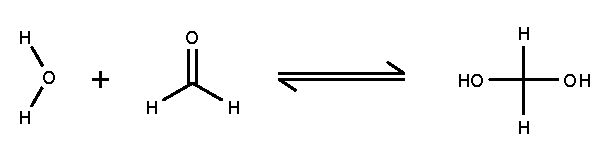
\includegraphics[width=0.6\textwidth]{formaldehyde1}
  \caption{Hydration of formaldehyde in water into methanediol}
  \label{fig:formal1}
\end{figure}

\subsection{The most common mechanism of the reaction}

A closer look at the reaction in Figure~\ref{fig:formal1} shows that the most common sequence 
of intermediate reactions leading to methanediol is the one given in Figure~\ref{fig:formal2}.
We now describe carefully its steps. The oxygen atom in one of the water molecules attacks the central 
carbon in the formaldehyde to form the intermediate 2 in Figure~\ref{fig:formal2}. Then one 
of the hydrogens of the positively charged oxygen is taken away by another water molecule 
in a proton transfer. This gives the intermediate 3. Finally, a proton is donated to the other 
oxygen in the intermediate 3 to give the final configuration 4.

\begin{figure}[h!]
  \centering
    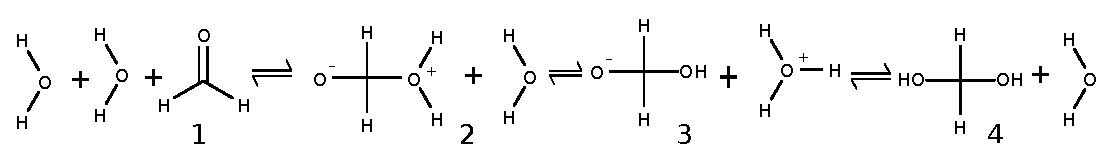
\includegraphics[width=1\textwidth]{formaldehyde2}
  \caption{The most common path through the hydration of formaldehyde}
  \label{fig:formal2}
\end{figure}

In order to model this reaction we need to understand what it is that makes it happen. 
The main factor is that the oxygen in the water is nucleophilic: it
tends to connect to another atomic nucleus. In the formaldehyde the oxygen attracts 
electrons towards itself, 
so the carbon has a positive charge. Now the oxygen in the water is attracted by this carbon 
and, due to its nucleophilicity, it forms a bond to the carbon. This bond is formed out of the electrons of one of the electrons in the oxygen so far not involved in bonding, so-called lone electron pairs. 
Since the carbon cannot have more than four bonds this reaction is compensated by 
the double bond in the formaldehyde becoming a single bond and the electrons from the double bond 
forming a lone pair on the oxygen, which now has three lone pairs. These movements are 
\emph{concerted}, namely they happen together without a stable intermediate state
and cannot be separated. So we have a continuous change between two tetracoordinate species through a pentacoordinate intermediate.  We have now reached the intermediate 2 in Figure~\ref{fig:formal2}. 

Looking at the intermediate 2, we can see that this has one oxygen which is negatively charged, 
because it has three lone pairs and a surplus of one electron. The other oxygen is positively 
charged, since it has three bonds and only one lone pair, therefore is missing an electron. 
The intermediate 2 reacts then with a water molecule. The water molecule is nucleophilic 
and has lone pairs for a bonding. It therefore can abstract one of the hydrogens on 
the positively charged oxygen. This leads to the intermediate 3 and a $\mathrm{H_3O}$ molecule, 
a water with an additional hydrogen and a positively charged oxygen.

Finally, a hydrogen can be re-donated to the negatively charged oxygen. Note that the re-donated 
hydrogen may not be the one which was originally attached to the oxygen. This transfer 
is possible since the oxygen in the $\mathrm{H_30}$ is electron-deficient and the negative oxygen 
is rich in electrons. We then get the substrate 4 which contains the final product 
methanediol, and water.

\subsection{Other paths through the reaction}
\label{sec:otherpaths}

There are other paths through the reaction of formaldehyde and water.
We assume that we now have a mixture of three water molecules and one formaldehyde molecule. 
This shall allow us to explore all other water-formaldehyde interactions. Two water molecules can interact 
to form $\mathrm{H_3O}$ and $\mathrm{HO}$. This is known as \emph{autoprotolysis of water} and is
described in detail in \cite{merevcomp2015}. These two molecules can be considered an acid and a base
respectively\footnote{There are slightly different definitions of acids and bases in the literature,
we use the general Bronsted-Lowry acid-base theory, which defines a base as a proton acceptor and 
an acid as a proton donor.}. Both bases and acids can interact with formaldehyde 
and thus produce methanediol by different mechanisms than those in the previous section.

\begin{figure}[h!]
  \centering
    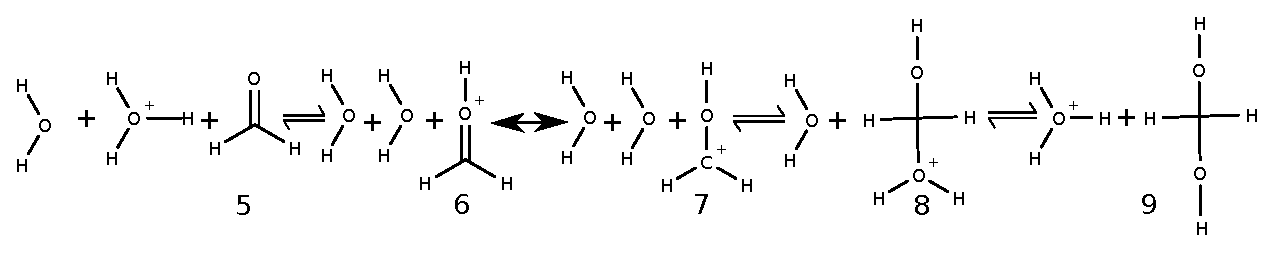
\includegraphics[width=1.0\textwidth]{formaldehyde_acid}
  \caption{Acid-catalysed hydration of formaldehyde in water.}
  \label{fig:acidcat}
\end{figure}

The acid-catalysed reaction is described in Figure~\ref{fig:acidcat}. Here the $\mathrm{H_3O}$ molecule,
which was formed during the autoprotolysis serves as the acid as it easily donates a proton. 
This proton can be donated to the oxygen in the formaldehyde, since this is slightly negatively charged, 
as we have seen. We then get the intermediate 6 in Figure~\ref{fig:acidcat}. The charge on the oxygen 
can ``move'' to the carbon by the electrons forming the bonds a lone pair on the oxygen. 
The real charge distribution is somewhere in between. We shall assume that the intermediates 6 and 7 
are somewhat  different structures, and we shall model the transition from 6 to 8 as a pair of 
concerted actions. Once the intermediate 8 is reached one of the protons from the oxygen in the
intermediate 8 can be abstracted by one of the water molecules, giving $\mathrm{H_3O}$ and
making it a catalytic process.

\begin{figure}[h!]
  \centering
    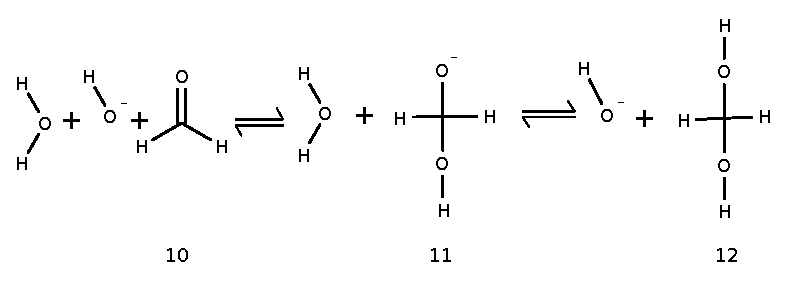
\includegraphics[width=0.7\textwidth]{formaldehyde_base}
  \caption{Base-catalysed hydration of formaldehyde in water.}
  \label{fig:basecat}
\end{figure}

The base-catalysed reaction in Figure~\ref{fig:basecat} starts with a water and a $\mathrm{HO^-}$ molecule, 
the base, which tends to accept protons very strongly. It can therefore interact with the carbon 
in the formaldehyde, which is similar to the water attacking the carbon. 
One of the bonds of the carbon-oxygen double bond is broken and the oxygen becomes negatively charged. 
This gives the intermediate 11 which is in fact the same as the intermediate 3 in 
Figure~\ref{fig:formal2}.
Then one of the protons of the water can be abstracted, and we obtain the methanediol and an 
$\mathrm{HO^⁻}$ molecule. Although this is the same structure as the original acid, it is made up 
from different atoms.  The process is considered catalytic since the $\mathrm{HO^⁻}$  molecule 
is retrieved at the end of the process.
\begin{figure}[h!]
\centering
      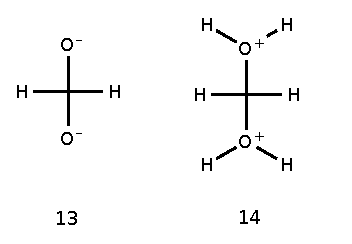
\includegraphics[width=.35\textwidth]{formaldehyde72}
        \caption{Other compounds possible in the reaction of formaldehyde with water.}
  \label{fig:misc}
\end{figure}

There are other ways that several molecules of water can react with formaldehyde to produce methanediol
and other byproducts. For example the base, $\mathrm{HO⁻}$, could directly interact with intermediate 7 
to form methanediol and two water molecules. 
Also, the two compounds given in Figure~\ref{fig:misc} can be created as intermediate products 
in the reaction. 

All possible reactions of a system of one formaldehyde and three water molecules are shown in
Figure~\ref{fig:formalallreal}. Although the direction of reactions are denoted with arrows, all 
reactions are reversible; the arrows merely indicate the direction to the final product.
We write FA for formaldehyde, W for water and MD for methanediol. Many of the intermediate compounds
are denoted by iX where $\mathrm{X}\in\{2,3,6,7,8,13,14\}$. 
Figure~\ref{fig:formalallreal} includes all intermediates from Figure~\ref{fig:acidcat} and 
Figure~\ref{fig:basecat}. The compounds in Figure~\ref{fig:misc} have only one path leading to them, 
and we could only move away from them by 
reverting these actions. This is because these compounds are the ``extreme'' states where there is 
either no hydrogen on an oxygen or both oxygens are fully saturated with two hydrogens. 
The resonance  between the intermediates i6 and i7 in Figure~\ref{fig:acidcat}  is represented 
by a dashed arrow.

\begin{figure}[t]
\psfrag{fawww}{${\mathrm{FA \paral W \paral W \paral W}}$}
\psfrag{fawhoh3o}{${\mathrm{FA \paral W \paral HO \paral H_3O}}$}
\psfrag{i6whow}{${\mathrm{i6 \paral W \paral HO \paral W}}$}
\psfrag{i8how}{${\mathrm{i8 \paral HO \paral W}}$}
\psfrag{mdhoh3o}{${\mathrm{MD \paral HO \paral H_3O}}$}
\psfrag{i2ww}{${\mathrm{i2 \paral W \paral W}}$}
\psfrag{i3h3ow}{${\mathrm{i3 \paral H_3O \paral W}}$}
\psfrag{mdww}{${\mathrm{MD \paral W \paral W}}$}
\psfrag{i6hohoh3o}{${\mathrm{i6 \paral HO \paral HO \paral H_3O}}$}
\psfrag{i7hohoh3o}{${\mathrm{i7 \paral HO \paral HO \paral H_3O}}$}
\psfrag{i7whow}{${\mathrm{i7 \paral W \paral HO \paral W}}$}
\psfrag{i14hoho}{${\mathrm{i14 \paral HO \paral HO}}$}
\psfrag{i13h3oh3o}{${\mathrm{i13 \paral H_3O \paral H_3O}}$}
\psfrag{i2hoh3o}{${\mathrm{i2 \paral H_3O \paral H_3O}}$}
  \centering
    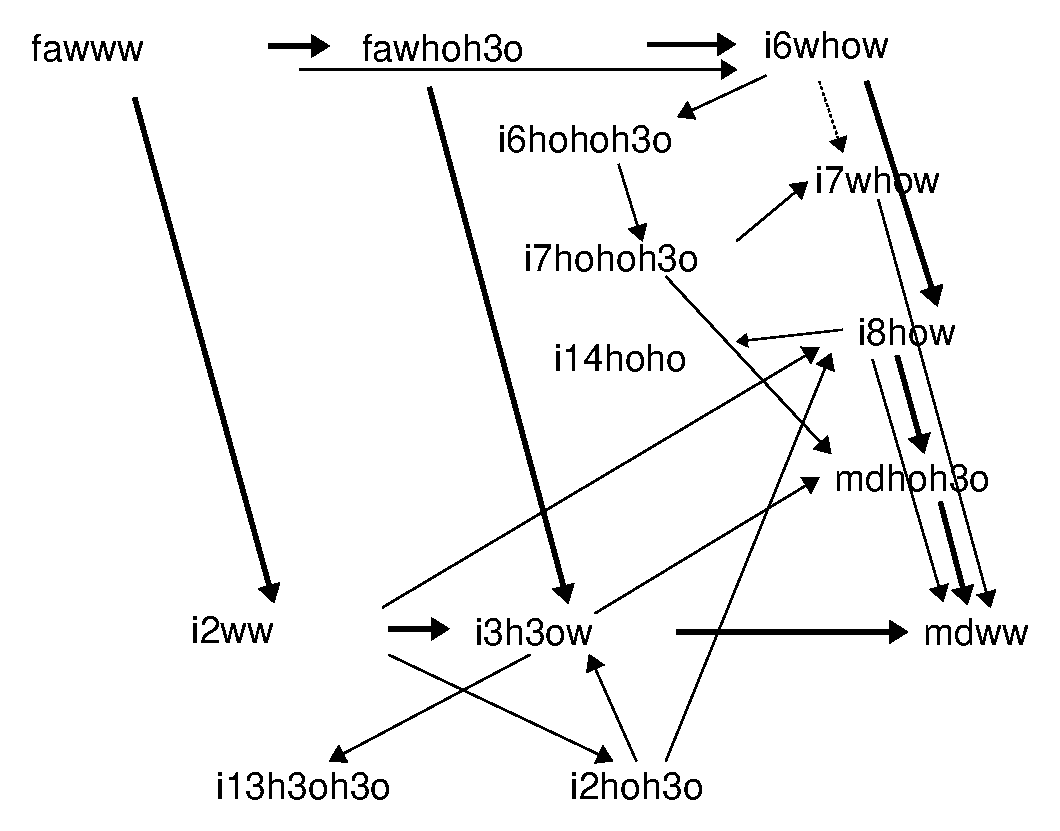
\includegraphics[width=1.0\textwidth]{formal_all_real2}
\caption{All possible reactions in a system of formaldehyde and three water molecules. 
The reactions displayed in more detail in Figure~\ref{fig:formal_graph} are denoted here by bold
arrows.}
  \label{fig:formalallreal}
\end{figure}

\Comment{
If, as it is normally done, the three possibilities are given separately, only the necessary molecules are taken into consideration. This is what we have done in Figure~\ref{fig:acidcat} and Figure~\ref{fig:basecat}, where only the base respectively acid and one water is shown. In our overall system we always have one water, one base and one acid. This means we get some additional paths. For example the base, $\mathrm{HO⁻}$, could directly interact with intermediate 7 to form methanediol and 2 water molecules. Figure~\ref{fig:formalallreal} shows all possible reactions in a system of formaldehyde and three water molecules. Actions are marked with an arrow to go from formaldehyde to methanediol, but all reactions are reversible. Figure~\ref{fig:formalallreal} includes all intermediates from Figure~\ref{fig:acidcat} and Figure~\ref{fig:basecat}. In addition two compounds given in Figure~\ref{fig:misc} can be created. These compounds have only one path leading to them, and we could only move away from them by reverting these actions. This is because these compounds are the ``extreme'' states where there is either no hydrogen on an oxygen or both oxygens are fully saturated with two hydrogens. In compounds where the two oxygens have different numbers of hydrogens we get different actions depending on which oxygen is involved. 
}

\Comment{
Figure~\ref{fig:formalallreal} is compiled from a chemical point of view - the nodes represent identical compounds. If these are identical processes in our calculus as well is not guaranteed. We will explore this difference in Section~\ref{sec:ccbwithsubscripts} further.

Notice there are other paths our calculus would enable. One example is an interaction of the methanediol, the final product, with a water molecule. Since the carbon has the action $p$ ready to perform and the oxygen in the water the action $n$ and $p,n$ is part of our synchronisation function there is nothing stopping this to happen. We have actually used a similar mechanism to get from 1 to 2 in Figure~\ref{fig:formal2}. A reason why this is not happening with methanediol is that the four groups around the carbon shield it from any interaction (as opposed to the three groups on the formaldehyde, of which two are relatively small hydrogens). So this is prevented by steric effect, effects due to atoms occupying space and preventing other atoms from moving.
}

\section{A CCB model of the hydration of formaldehyde in water}
\label{sec:formaldehydemodel}
We are now ready to model our reaction in CCB.
Figure~\ref{fig:formal_graph} shows in more detail the three main paths through our reaction 
that we described in the last section; these paths have been highlighted in bold in 
Figure~\ref{fig:formalallreal}. 

The initial state of the reaction is modelled by the composition of one 
formaldehyde FA three waters, written as $\mathrm{FA \paral W \paral W \paral W}$. 
The final products are methanediol $\mathrm{MD}$ and two waters,
written as $\mathrm{MD \paral W \paral W}$. The path via the intermediate molecules 2 and 3 
in Figure~\ref{fig:formal2} is via the nodes denoted by i2 and i3 in Figure~\ref{fig:formal_graph}.
The $\mathrm{FA \paral W \paral HO \paral H_3O}$ 
node is the result of an autoprotolysis. The base-catalysed and acid-catalysed reactions 
are put into the same diagram, again the intermediates i6 and i8 correspond to molecules 
in Figure~\ref{fig:acidcat}. 
%
%The subscripts in the transitions refer to the modelling done in the next paragraph. 
%
As we can see in Figure~\ref{fig:formal_graph} the reactions are driven completely by 
concerted actions. 
%
%TODO: We note that the transition from the intermediate 6 to 8 is somewhat
%different to other transitions, and may need to be represented more specifically in the future. 
%The remaining transitions are handled as concerted actions by our calculus.

\begin{figure}[t]
\psfrag{l1}{${\scriptstyle\{np[11],\underline{c_4o_2}[4]\}}$}
\psfrag{l2}{${\scriptstyle\{np[12],\underline{h_3o_3}[5]\}}$}
\psfrag{l3}{${\scriptstyle\{np[13],\underline{h_5o_5}[12]\}}$}
\psfrag{l4}{${\scriptstyle\{np[12],\underline{h_3o_3}[5]\}}$}
\psfrag{l5}{${\scriptstyle\{np[11],\underline{c_4o_2}[4]\}}$}
\psfrag{l6}{${\scriptstyle\{np[13],\underline{h_5o_5}[7]\}}$}
\psfrag{l7}{${\scriptstyle\{np[11],\underline{c_4o_2}[4]\}}$}
\psfrag{l8}{${\scriptstyle\{np[14],\underline{h_6o_6}[8]\}}$}
\psfrag{l9}{${\scriptstyle\{np[5],\underline{h_8o_8}[14]\}}$}

\psfrag{fawww}{${\mathrm{FA \paral W \paral W \paral W}}$}
\psfrag{fawhoh3o}{${\mathrm{FA \paral W \paral HO \paral H_3O}}$}
\psfrag{i6whow}{${\mathrm{i6 \paral W \paral HO \paral W}}$}
\psfrag{i8how}{${\mathrm{i8 \paral HO \paral W}}$}
\psfrag{mdhoh3o}{${\mathrm{MD \paral HO \paral H_3O}}$}
\psfrag{i2ww}{${\mathrm{i2 \paral W \paral W}}$}
\psfrag{i3h3ow}{${\mathrm{i3 \paral H_3O \paral W}}$}
\psfrag{mdww}{${\mathrm{MD \paral W \paral W}}$}

\centering
    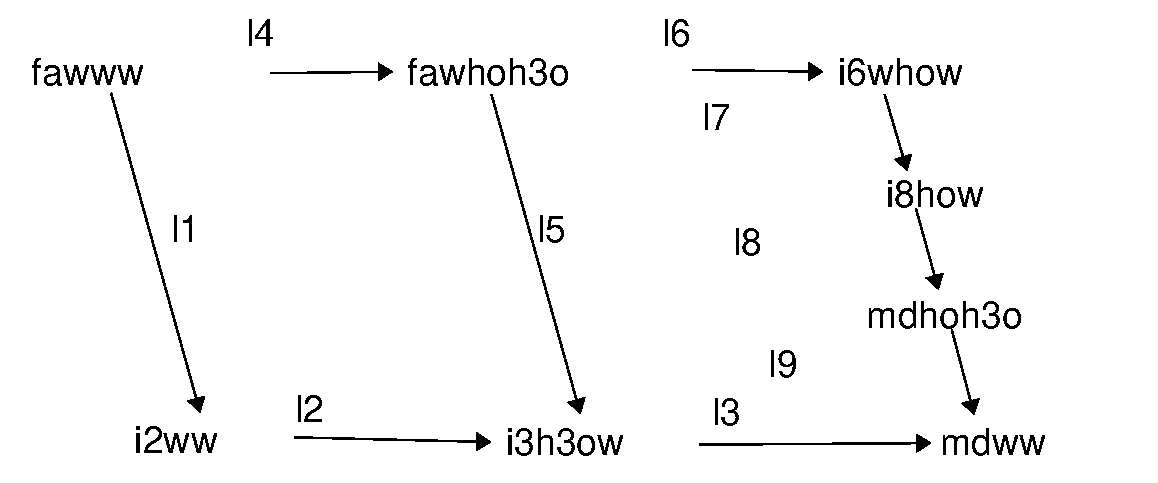
\includegraphics[width=1.0\textwidth]{formal_all}
\caption{The three main reaction paths in the hydration of formaldehyde.}
\label{fig:formal_graph}
\end{figure}

We model the formaldehyde molecule $\mathrm{CH_2O}$ and the three water molecules $\mathrm{H_2O}$
as appropriate compositions of their atoms, namely hydrogen, oxygen and carbon. We use our 
general prefixing operator to define these atoms: 
$$\begin{array}{lll}
H & \bydef & (h;p).H'\\
O & \bydef & (o,o,n).O'\\
C & \bydef & (c,c,c,c;p).C'
\end{array}$$
Carbon has four strong actions $c$, representing the potential for four covalent bonds, and 
a weak action $p$, standing for a positive partial charge. 
The oxygen can have up to three bonds. Normally is has two bonds, however, if a suitable reaction 
partner is close, an additional weak bond is available. We use therefore the simple prefixing operator
to model it, with one weak action $n$ standing for the potential for a negative partial charge. 
A partial charge means that a part or parts of a molecule have an electric charge, even though 
the molecule as a whole is neutrally charged. These uneven charge distributions enable 
many reactions by allowing another molecule to attack a partially charged part.
The hydrogen has one strong bond, and we use additionally a weak action $p$ to represent 
that it can become positively charged. Processes $H'$, $O'$, and $C'$ represent 
unspecified further behaviour of the respective atoms.

Since our reaction involves multiple copies of $H$ and $O$ we shall adopt a subscript notation 
to denote distinct copies of the same process. Both action labels and process names will be
subscripted. For example, $H_1\bydef (h_1;p).H_1'$ and $H_2\bydef (h_2;p).H_2'$ are two copies
of hydrogen $H$. 
We shall abstract away these subscripts in Section~\ref{chem-eq}, where we introduce
informally chemical equivalence.  
Also, the copies of actions $c$ of carbon will also be subscripted.
% to ``tell them apart". 

The synchronisation function $\gamma$ is defined on subscripted actions as follows:
%
$$\begin{array}{ l c l l }
\gamma(c_i,h_j) & = & c_ih_j \quad & i \in \{1,\ldots, 4\}, j\in\{1,\ldots,8\} \\
\gamma(h_i,o_j) & = & h_io_j \quad & i \in \{1,\ldots, 8\}, j\in\{1,\ldots,6\}  \\
\gamma(c_i,o_j) & = & c_io_j \quad & i \in \{1,\ldots, 4\}, j\in\{1,\ldots,6\} \\
\gamma(c_i,n) & = & c_in & i \in \{1,\ldots, 4\} \\
\gamma(h_i,n) & = & h_in & i \in \{1,\ldots,8\}  \\
\gamma(n,p) & = & np &  \\
\end{array}$$
Now we are ready to model $\mathrm{H_2O}$ and $\mathrm{CH_2O}$ molecules. A water molecule is modelled 
simply as a composition of two copies of the hydrogen process with one copy of oxygen; see below. 
%
\Comment{
\Stefan{The restrictions ensure that the molecules form as desired and once they exist only 
communications on weak actions $n$ and $P$ happen.  Of course the atoms could react to form another 
set of molecules, but we assume a particular set of initial reactions to get the starting molecules 
for our reaction.} 
}
The restriction of actions $h_i$ and $o_i$, for $i\in\{3,4\}$, ensures that actions such as 
$h_3[5]$ cannot be undone alone but only together with their partners $o_3[5]$. This happens via
undoing of $h_3o_3[5]$ bond. Correspondingly, when
any of these actions is fresh they can only happen together with their partners (as prescribed by
the communication function $\gamma$), and not alone. 
We also restrict $np$ to stop self-bonding of water's hydrogens with its oxygen.
%and that we do not allow $n$ and $p$ to bond, or refer to RC15 paper
%
$$\begin{array}{l}
((h_3[5];p).H'_3 \paral (h_4[6];p).H'_4 \paral (o_3[5],o_4[6],n).O'_2)
  \setminus\{h_3,h_4,o_3,o_4, np\} \\
\end{array}$$
The formaldehyde molecule is modelled by
$$\begin{array}{l}
(((c_1[1],c_2[2],c_3[3],c_4[4];p).C' \paral (h_1[1];p).H'_1 \paral (h_2[2];p).H'_2 \paral
(o_1[3],o_2[4],n).O'_1)\\
  \quad \setminus\{c_1,c_2,c_3,c_4,h_1,h_2,o_1,o_2,np,\underline{c_{1}h_{1}}, \underline{c_{2}h_{2}},
  \}
\end{array}$$
We restrict the appropriate versions of the $c_i, o_j$ and $h_k$ actions, for
all $i,j$ and $k$, meaning that we do not allow the creation of new bonds (involving these actions)
between different molecules as single acts of synchronisation. Such new bonds will be created
via concerted actions and (almost) always via the weak $np$ bonds which will then get promoted
to strong bonds.

We also restrict $\underline{c_i h_i}$ for $i\in\{1,2\}$. It prevents
breaking any of the bonds between $C_1$ and its hydrogens $H_1$ and $H_2$.
This serves two purposes. Firstly, it makes sure that once we have done the $p$ action of
the carbon, we will break one of the bonds between the carbon and the oxygen. This is justified
since in reality it is one of the oxygen bonds which is broken, so this models the reality closely.
Secondly, it also prevents $O_2$ or $O_3$ from abstracting $H_1$ or $H_2$ from the carbon.
Note that $\underline{h_i}$, $\underline{o_j}$ and $\underline{n}$ are not restricted in FA and 
in W: this allows us to break bonds involving these actions as a part of concerted
actions.

The four molecules of the reaction are now composed in parallel:
$$(\mathrm{CH_2O \paral H_2O \paral H_2O \paral H_2O})\setminus \{n,p\}$$
We restrict actions $n$ and $p$, so that they
cannot happen separately from each other but only together within this system of processes. 

The main path through the reaction require only two copies of water so we start 
with the following initial state, where keys $1, \ldots, 8$ specify the existing
initially bonds of formaldehyde and the two waters.
\begin{flalign*}
&(((c_1[1],c_2[2],c_3[3],c_4[4];p).C' \paral (h_1[1];p).H'_1 \paral (h_2[2];p).H'_2 \paral 
(o_1[3],o_2[4],n).O'_1) \\
 & \qquad  \setminus\{c_1,c_2,c_3,c_4,h_1,h_2,o_1,o_2,np,\underline{c_{1}h_{1}}, \underline{c_{2}h_{2}}\} \\
&\paral ((h_3[5];p).H'_3 \paral (h_4[6];p).H'_4 \paral (o_3[5],o_4[6],n).O'_2) 
  \setminus\{h_3,h_4,o_3,o_4,np\} \\
&\paral ((h_5[7];p).H'_5 \paral (h_6[8];p).H'_6 \paral (o_5[7],o_6[8],n).O'_3) 
  \setminus\{h_5,h_6,o_5,o_6,np\} ) \; \setminus \{n,p\}
\end{flalign*}
%
In order to simplify the display of transitions or rewrites of this process we omit the four
restrictions and write the initial process simply as
%
\begin{flalign*}
&(c_1[1],c_2[2],c_3[3],c_4[4];p).C' \paral (h_1[1];p).H'_1 \paral (h_2[2];p).H'_2 \paral (o_1[3],o_2[4],n).O'_1 
   \\
&\paral (h_3[5];p).H'_3 \paral (h_4[6];p).H'_4 \paral (o_3[5],o_4[6],n).O'_2 
   \\
&\paral (h_5[7];p).H'_5 \paral (h_6[8];p).H'_6 \paral (o_5[7],o_6[8],n).O'_3 
%\; \setminus L
\end{flalign*}
%where $L=\{c_1,c_2,c_3,c_4,h_1,h_2,h_3,h_4,h_5,h_6,o_1,o_2,o_3,o_4,o_5,o_6,n,p,
%\underline{c_{1}h_{1}}, \underline{c_{2}h_{2}}\}$.
remembering that the restrictions are still there.

\subsection{The main path through the reaction}
We first consider the reaction steps in Figure~\ref{fig:formal2}, following the path via 
$\mathrm{i3 \paral H_3O \paral W}$ and $\mathrm{i2 \paral W \paral W}$
in Figures~\ref{fig:formalallreal} and \ref{fig:formal_graph}. The first step is the $n,p$ 
reaction between $C_1$ and $O_2$ or $O_3$. 
Note that there are other $n,p$ reactions that are allowed by our model. 
%
% introducing a restriction of np stops this now:
\Comment{For example, the $n,p$ reaction between $O_1$ and $C$. 
If $O_1$ reacted with $C$, this would force the breaking of one of 
the bonds $1,\ldots,4$ of the carbon. Since restriction of $\underline{c_i h_i}$, for $i\in\{1,2\}$,
prevents dissolving of bonds 1 and 2, one of the bonds 3 or 4 will be broken. So, we will
end up with two bonds between $C$ and $O_1$ as before. Hence, this would not lead to an
effective change, so this case is omitted.
}
We could have $O_2$ getting a hydrogen from $O_3$,
or vice versa, which is the autoprotolysis of water which we have mentioned before. 
We shall discuss this 
further later on. Also $O_1$ could pull one of the hydrogens from one of the water molecules:
again we shall discuss it later. 

Returning to the first step of our reaction, we have 
$O_2$ bonding with $C$ with the key $11$. This is followed immediately by breaking of the bond 3 or 4 
by the rule \rulename{concert}.
% applied to a process of the form $(s;b).P$ in parallel with another process. 
Note that
breaking of 1 or 2 is not possible because of the restriction of $c_1h_1$ and $c_2h_2$. 
We break the bond 4 and get a transition by concerted actions: 
we create the bond $np[11]$ and break the bond $\underline{c_4o_2}[4]$. Henceforth
we shall write the name of the target of a transition below the transition,
using the names that appear in Figures~\ref{fig:formalallreal}-\ref{fig:formal_graph}.
Here, for example, the compound resulting from
this transition is $\mathrm{i2 \paral W }$ but since in general we have an extra water W,
we write $\mathrm{i2 \paral W \paral W}$.
\begin{flalign*}
&\xrightarrow{\{np[11],\underline{c_4o_2}[4]\}}
	(c_1[1],c_2[2],c_3[3],c_4;p[11]).C' \paral (h_1[1];p).H'_1 \paral (h_2[2];p).H'_2 \paral \\
&\qquad (o_1[3],o_2,n).O'_1 \paral (h_3[5];p).H'_3 \paral (h_4[6];p).H'_4 \paral (o_3[5],o_4[6],n[11]).O'_2 \\
&\paral (h_5[7];p).H'_5 \paral (h_6[8];p).H'_6 \paral (o_5[7],o_6[8],n).O'_3 % ) \setminus L \qquad 
\end{flalign*}
\hfill{$\mathrm{i2 \paral W \paral W}$}
\\
Now the \rulename{prom} rewrite rule must be applied before we derive the next concerted transition: we promote 
the weak bond 11 of the carbon to a stronger bond on $c_4$, which has become available:
%
\begin{flalign*}
&\Tran{} \; ((c_1[1],c_2[2],c_3[3],c_4[11];p).C' \paral (h_1[1];p).H'_1 \paral (h_2[2];p).H'_2  \\
&\paral (o_1[3],o_2,n).O'_1 \paral (h_3[5];p).H'_3 \paral (h_4[6];p).H'_4 \paral (o_3[5],o_4[6],n[11]).O'_2 \\
&\paral (h_5[7];p).H'_5 \paral (h_6[8];p).H'_6 \paral (o_5[7],o_6[8],n).O'_3 ) \setminus L \qquad
\end{flalign*}
\hfill{$\mathrm{i2 \paral W \paral W}$}
\\
%We note that $O_1$ is now negatively charged (it has only one bond), but we do not need to 
%consider it to get our desired result. 
The next step is to form a bond between $O_3$ and
either $H_3$ or $H_4$. We bond with $H_3$ with the key 12 and break the bond 5, producing a pair
of concerted actions. We then move a weak bond 11 on $n$ in $O_2$ to a stronger bond
on $o_3$ (which has become available) by rewrite rule move-r. We also promote the weak bond 12 in $H_3$ 
to a strong bond on $h_3$ by rewrite rule \rulename{prom}, giving overall this transition:
%
\begin{flalign*}
&\xrightarrow{\{np[12],\underline{h_3o_3}[5]\}}
	(c_1[1],c_2[2],c_3[3],c_4[11];p).C' \paral (h_1[1];p).H'_1 \paral (h_2[2];p).H'_2 \paral \\
&\qquad (o_1[3],o_2,n).O'_1 \paral (h_3[12];p).H'_3 \paral (h_4[6];p).H'_4 \paral (o_3[11],o_4[6],n).O'_2 \\
&\paral (h_5[7];p).H'_5 \paral (h_6[8];p).H'_6 \paral (o_5[7],o_6[8],n[12]).O'_3 %) \setminus L \qquad 
\end{flalign*}
\hfill{$\mathrm{i3 \paral H_3O \paral W}$}
\\

The next step is a proton transfer from $O_3$ to $O_1$. We transfer $H_5$ (but we could have used 
$H_6$ or $H_3$ since they all have the $p$ action ready). 
%That also $H_3$ can do so is thanks to our new calculus, since it has done some actions before, 
%but appears the same as the other hydrogens bonded to $O_3$. 
Performing the transfer of $H_5$ from $O_3$ to $O_1$ (and breaking the bond 12), we obtain the following:
%
\begin{flalign*}
&\xrightarrow{\{np[13],\underline{h_5o_5}[12]\}}
	(c_1[1],c_2[2],c_3[3],c_4[11];p).C' \paral (h_1[1];p).H'_1 \paral (h_2[2];p).H'_2 \paral \\
&\qquad (o_1[3],o_2,n[13]).O'_1 \paral (h_3;p[13]).H'_3 \paral (h_4[6];p).H'_4 \paral (o_3[11],o_4[6],n).O'_2 \\
&\paral (h_5[7];p).H'_5 \paral (h_6[8];p).H'_6 \paral (o_5[7],o_6[8],n).O'_3 %) \setminus L \qquad 
\end{flalign*}
\hfill{$\mathrm{MD \paral W \paral W}$}
\\
and promoting and moving the bond 13 in $H_3$ and $O_1$, respectively, to strong bonds 
we obtain the final product (methanediol $\mathrm{CH_2(OH)_2}$) and two waters:
%
\begin{flalign*}
	&\Tran{}\ (c_1[1],c_2[2],c_3[3],c_4[11];p).C' \paral (h_1[1];p).H'_1 \paral (h_2[2];p).H'_2\\
& \paral (o_1[3],o_2[13],n).O'_1 \paral (h_3[13];p).H'_3 \paral (h_4[6];p).H'_4 \paral (o_3[11],o_4[6],n).O'_2 \\
&\paral (h_5[7];p).H'_5 \paral (h_6[8];p).H'_6 \paral (o_5[7],o_6[8],n).O'_3 %) \setminus L \qquad
\end{flalign*}
\hfill{$\mathrm{MD \paral W \paral W}$}
%

\noindent
Note that the $n,p$ actions are ready again and all the existing bonds are on strong actions. 
So we now can reverse the reaction by $O_3$ abstracting a hydrogen from $H_4$ or $H_5$, and 
all the way to the initial state.
Moreover, let us inspect the bonds 4, 5 and 7 which are broken during the reaction. The bonds were formed during the initial bonding of the atoms. They are broken as a
result of application of our new general prefixing operator. This operator enables the reaction 
to work forwards without external control. Indeed the original order of the formation of 
the bonds is completely irrelevant for the reaction to work.

\subsection{The base-catalysed path}

We now consider the base-catalysed path described in Figure~\ref{fig:basecat}. The path is via  
$\mathrm{FA \paral W \paral HO \paral H_3O}$ and  $\mathrm{i3 \paral H_3O \paral W}$  to
$\mathrm{MD \paral W \paral W}$ in Figures~\ref{fig:formalallreal}-\ref{fig:formal_graph}. 
The path needs three water molecules. We shall show the application of the promotion or move 
rules without explaining them in detail. We start with the initial system (remembering that
restrictions are not shown):
\begin{flalign*} 
&(c_1[1],c_2[2],c_3[3],c_4[4];p).C' \paral (h_1[1];p).H'_1 \paral (h_2[2];p).H'_2 \paral 
	(o_1[3],o_2[4],n).O'_1 \\
&\paral (h_3[5];p).H'_3 \paral (h_4[6];p).H'_4 \paral (o_3[5],o_4[6],n).O'_2 
   \\
&\paral (h_5[7];p).H'_5 \paral (h_6[8];p).H'_6 \paral (o_5[7],o_6[8],n).O'_3 
   \\
&\paral (h_7[9];p).H'_7 \paral (h_8[10];p).H'_8 \paral (o_7[9],o_8[10],n).O'_4 
  %\; \setminus L \qquad 
\end{flalign*}
\hfill{$\mathrm{FA \paral W \paral W \paral W}$}
\\
%
\noindent
\begin{flalign*}
&\xrightarrow{\{np[12],\underline{h_3o_3}[5]\}}(c_1[1],c_2[2],c_3[3],c_4[4];p).C' \paral (h_1[1];p).H'_1 \paral (h_2[2];p).H'_2   \\
& \paral (o_1[3],o_2[4],n).O'_1 \paral (h_3;p[12]).H'_3 \paral (h_4[6];p).H'_4 \paral (o_3,o_4[6],n).O'_2 
   \\
&\paral (h_5[7];p).H'_5 \paral (h_6[8];p).H'_6 \paral (o_5[7],o_6[8],n[12]).O'_3 
   \\
&\paral (h_7[9];p).H'_7 \paral (h_8[10];p).H'_8 \paral (o_7[9],o_8[10],n).O'_4 
  %\; \setminus L \qquad
\end{flalign*}
%\hfill{$\mathrm{FA \paral W \paral HO \paral H_3O}$}
%\\
\begin{flalign*}
&\Tran{}(c_1[1],c_2[2],c_3[3],c_4[4];p).C' \paral (h_1[1];p).H'_1 \paral (h_2[2];p).H'_2
   \\
& \paral (o_1[3],o_2[4],n).O'_1 \paral (h_3[12];p).H'_3 \paral (h_4[6];p).H'_4 \paral (o_3,o_4[6],n).O'_2 
   \\
&\paral (h_5[7];p).H'_5 \paral (h_6[8];p).H'_6 \paral (o_5[7],o_6[8],n[12]).O'_3 
   \\
&\paral (h_7[9];p).H'_7 \paral (h_8[10];p).H'_8 \paral (o_7[9],o_8[10],n).O'_4 
  %\; \setminus L \qquad
\end{flalign*}
\hfill{$\mathrm{FA \paral W \paral HO \paral H_3O}$}
\\
\begin{flalign*}
&\xrightarrow{\{np[11],\underline{c_4o_4}[4]\}}(c_1[1],c_2[2],c_3[3],c_4;p[11]).C' \paral (h_1[1];p).H'_1 \paral (h_2[2];p).H'_2 
   \\
& \paral (o_1[3],o_2,n).O'_1 \paral (h_3[12];p).H'_3 \paral (h_4[6];p).H'_4 \paral (o_3,o_4[6],n[11]).O'_2 
   \\
&\paral (h_5[7];p).H'_5 \paral (h_6[8];p).H'_6 \paral (o_5[7],o_6[8],n[12]).O'_3 
   \\
&\paral (h_7[9];p).H'_7 \paral (h_8[10];p).H'_8 \paral (o_7[9],o_8[10],n).O'_4 
  %\; \setminus L \qquad
\end{flalign*}
%\hfill{$\mathrm{i3 \paral H_3O \paral W}$}
%\\
\begin{flalign*}
	&\Tran{}(c_1[1],c_2[2],c_3[3],c_4[11];p).C' \paral (h_1[1];p).H'_1 \paral (h_2[2];p).H'_2 
   \\
& \paral (o_1[3],o_2,n).O'_1 \paral (h_3[12];p).H'_3 \paral (h_4[6];p).H'_4 \paral (o_3[11],o_4[6],n).O'_2 
   \\
&\paral (h_5[7];p).H'_5 \paral (h_6[8];p).H'_6 \paral (o_5[7],o_6[8],n[12]).O'_3 
   \\
&\paral (h_7[9];p).H'_7 \paral (h_8[10];p).H'_8 \paral (o_7[9],o_8[10],n).O'_4 
  %\; \setminus L \qquad
\end{flalign*}
\hfill{$\mathrm{i3 \paral H_3O \paral W}$}
\\
\begin{flalign*}
&\xrightarrow{\{np[13],\underline{h_3n}[12]\}}(c_1[1],c_2[2],c_3[3],c_4[11];p).C' \paral (h_1[1];p).H'_1 \paral (h_2[2];p).H'_2 
   \\
&\paral (o_1[3],o_2,n[13]).O'_1 \paral (h_3;p[13]).H'_3 \paral (h_4[6];p).H'_4 \paral (o_3[11],o_4[6],n).O'_2 
   \\
&\paral (h_5[7];p).H'_5 \paral (h_6[8];p).H'_6 \paral (o_5[7],o_6[8],n).O'_3 
   \\
&\paral (h_7[9];p).H'_7 \paral (h_8[10];p).H'_8 \paral (o_7[9],o_8[10],n).O'_4 
  %\; \setminus L \qquad
\end{flalign*}
%\hfill{$\mathrm{MD \paral W \paral W}$}
%\\
\begin{flalign*}
&\Tran{}(c_1[1],c_2[2],c_3[3],c_4[11];p).C' \paral (h_1[1];p).H'_1 \paral (h_2[2];p).H'_2
   \\
& \paral (o_1[3],o_2[13],n).O'_1 \paral (h_3[13];p).H'_3 \paral (h_4[6];p).H'_4 \paral (o_3[11],o_4[6],n).O'_2 
   \\
&\paral (h_5[7];p).H'_5 \paral (h_6[8];p).H'_6 \paral (o_5[7],o_6[8],n).O'_3
   \\
&\paral (h_7[9];p).H'_7 \paral (h_8[10];p).H'_8 \paral (o_7[9],o_8[10],n).O'_4 
  %\; \setminus L \qquad
\end{flalign*}
\hfill{$\mathrm{MD \paral W \paral W}$}
\\
We have reached the final state of the reaction: a methanediol with two waters. Notice 
that the methanediol
process is identical (including keys) to the  methanediol process in the main path.
%
\subsection{The acid-catalysed path}

Next we consider the acid-catalysed path described in Figure~\ref{fig:acidcat}. The path is via
$\mathrm{i6 \paral W \paral HO \paral W}$ and $\mathrm{i8 \paral HO \paral W}$ in 
Figures~\ref{fig:formalallreal}--\ref{fig:formal_graph}.  The path uses three water molecules 
as in the base-catalysed path. We shall apply the promotion or move rules as needed.
We start with the initial system:
\begin{flalign*}
&(c_1[1],c_2[2],c_3[3],c_4[4];p).C' \paral (h_1[1];p).H'_1 \paral (h_2[2];p).H'_2  
   \\
&\paral (o_1[3],o_2[4],n).O'_1 \paral (h_3[12];p).H'_3 \paral (h_4[6];p).H'_4 \paral (o_3,o_4[6],n).O'_2 
   \\
&\paral (h_5[7];p).H'_5 \paral (h_6[8];p).H'_6 \paral (o_5[7],o_6[8],n[12]).O'_3 
\\
&\paral (h_7[9];p).H'_7 \paral (h_8[10];p).H'_8 \paral (o_7[9],o_8[10],n).O'_4 %  \; \setminus L \qquad 
\end{flalign*}
\hfill{$\mathrm{FA \paral W \paral HO \paral H_3O}$}
\\
\begin{flalign*}
&\xrightarrow{\{np[13],\underline{h_5o_5}[7]\}}(c_1[1],c_2[2],c_3[3],c_4[4];p).C' \paral (h_1[1];p).H'_1 \paral (h_2[2];p).H'_2
   \\
& \paral (o_1[3],o_2[4],n[13]).O'_1 \paral (h_3[12];p).H'_3 \paral (h_4[6];p).H'_4 \paral (o_3,o_4[6],n).O'_2 
   \\
&\paral (h_5;p[13]).H'_5 \paral (h_6[8];p).H'_6 \paral (o_5,o_6[8],n[12]).O'_3 
\\
&\paral (h_7[9];p).H'_7 \paral (h_8[10];p).H'_8 \paral (o_7[9],o_8[10],n).O'_4  % \; \setminus L \qquad
\end{flalign*}
%\hfill{$\mathrm{i6 \paral W \paral HO \paral W}$}
%\\
\begin{flalign*}
&\Tran{}(c_1[1],c_2[2],c_3[3],c_4[4];p).C' \paral (h_1[1];p).H'_1 \paral (h_2[2];p).H'_2
   \\
& \paral (o_1[3],o_2[4],n[13]).O'_1 \paral (h_3[12];p).H'_3 \paral (h_4[6];p).H'_4 \paral (o_3,o_4[6],n).O'_2 
   \\
&\paral (h_5[13];p).H'_5 \paral (h_6[8];p).H'_6 \paral (o_5[12],o_6[8],n).O'_3 
   \\
&\paral (h_7[9];p).H'_7 \paral (h_8[10];p).H'_8 \paral (o_7[9],o_8[10],n).O'_4 %\; \setminus L \qquad
\end{flalign*}
\hfill{$\mathrm{i6 \paral W \paral HO \paral W}$}
\\
The last rewrite is by rule \rulename{move-r}. The reaction continues as follows:

\begin{flalign*}
&\xrightarrow{\{np[11], \underline{c_4o_2}[4]\}}(c_1[1],c_2[2],c_3[3],c_4;p[11]).C' \paral (h_1[1];p).H'_1 \paral (h_2[2];p).H'_2
   \\
   & \paral (o_1[3],o_2,n[13]).O'_1 \paral (h_3[12];p).H'_3 \paral (h_4[6];p).H'_4 \paral (o_3,o_4[6],n).O'_2 
   \\
&\paral (h_5[13];p).H'_5 \paral (h_6[8];p).H'_6 \paral (o_5[12],o_6[8],n[11]).O'_3 
\\
&\paral (h_7[9];p).H'_7 \paral (h_8[10];p).H'_8 \paral (o_7[9],o_8[10],n).O'_4   %\; \setminus L \qquad
\end{flalign*}
%\hfill{$\mathrm{i8 \paral HO \paral W}$}
%\\
\begin{flalign*}
&\Tran{}(c_1[1],c_2[2],c_3[3],c_4[11];p).C' \paral (h_1[1];p).H'_1 \paral (h_2[2];p).H'_2 
   \\
&\paral (o_1[3],o_2[13],n).O'_1 \paral (h_3[12];p).H'_3 \paral (h_4[6];p).H'_4 \paral (o_3,o_4[6],n).O'_2 
   \\
&\paral (h_5[13];p).H'_5 \paral (h_6[8];p).H'_6 \paral (o_5[12],o_6[8],n[11]).O'_3 
\\
&\paral (h_7[9];p).H'_7 \paral (h_8[10];p).H'_8 \paral (o_7[9],o_8[10],n).O'_4)   %\; \setminus L \qquad
\end{flalign*}
\hfill{$\mathrm{i8 \paral HO \paral W}$}
\\
\noindent
We continue from $\mathrm{i8 \paral HO \paral W}$ via $\mathrm{MD \paral HO \paral H_3O}$ 
with concerted actions:
\begin{flalign*}
&\xrightarrow{\{np[14],\underline{h_6o_6[8]}\}}(c_1[1],c_2[2],c_3[3],c_4[11];p).C' \paral (h_1[1];p).H'_1 \paral (h_2[2];p).H'_2
   \\
& \paral (o_1[3],o_2[13],n).O'_1 \paral (h_3[12];p).H'_3 \paral (h_4[6];p).H'_4 \paral (o_3,o_4[6],n).O'_2 
   \\
&\paral (h_5[13];p).H'_5 \paral (h_6;p[14]).H'_6 \paral (o_5[12],o_6,n[11]).O'_3 
 \\
&\paral (h_7[9];p).H'_7 \paral (h_8[10];p).H'_8 \paral (o_7[9],o_8[10],n[14]).O'_4%)   \; \setminus L \qquad 
\end{flalign*}
%\hfill{$\mathrm{MD \paral HO \paral H_3O}$}
%\\
\begin{flalign*}
&\Tran{}(c_1[1],c_2[2],c_3[3],c_4[11];p).C' \paral (h_1[1];p).H'_1 \paral (h_2[2];p).H'_2 
   \\
&\paral (o_1[3],o_2[13],n).O'_1 \paral (h_3[12];p).H'_3 \paral (h_4[6];p).H'_4 \paral (o_3,o_4[6],n).O'_2 
   \\
&\paral (h_5[13];p).H'_5 \paral (h_6[14];p).H'_6 \paral (o_5[12],o_6[11],n).O'_3 
  \\
&\paral (h_7[9];p).H'_7 \paral (h_8[10];p).H'_8 \paral (o_7[9],o_8[10],n[14]).O'_4%) \; \setminus L \qquad 
\end{flalign*}
\hfill{$\mathrm{MD \paral HO \paral H_3O}$}
\\
Finally we reach the final state of a methanediol and two waters:
\begin{flalign*}
&\xrightarrow{\{np[5],\underline{h_8o_8}[14]\}}(c_1[1],c_2[2],c_3[3],c_4[11];p).C' \paral (h_1[1];p).H'_1 \paral (h_2[2];p).H'_2
   \\
& \paral (o_1[3],o_2[13],n).O'_1 \paral (h_3[12];p).H'_3 \paral (h_4[6];p).H'_4 \paral (o_3,o_4[6],n[5]).O'_2 
   \\
&\paral (h_5[13];p).H'_5 \paral (h_6[14];p).H'_6 \paral (o_5[12],o_6[11],n).O'_3 
  \\
&\paral (h_7[9];p).H'_7 \paral (h_8;p[5]).H'_8 \paral (o_7[9],o_8[10],n[14]).O'_4%) 
\end{flalign*}
%\hfill{$\mathrm{MD \paral W \paral W}$}
%\\
\begin{flalign*}
&\Tran{}(c_1[1],c_2[2],c_3[3],c_4[11];p).C' \paral (h_1[1];p).H'_1 \paral (h_2[2];p).H'_2
   \\
& \paral (o_1[3],o_2[13],n).O'_1 \paral (h_3[12];p).H'_3 \paral (h_4[6];p).H'_4 \paral (o_3[5],o_4[6],n).O'_2 
   \\
&\paral (h_5[13];p).H'_5 \paral (h_6[10];p).H'_6 \paral (o_5[12],o_6[11],n).O'_3 
   \\
&\paral (h_7[9];p).H'_7 \paral (h_8[5];p]).H'_8 \paral (o_7[9],o_8[10],n).O'_4%) \; \setminus L \qquad 
\end{flalign*}
\hfill{$\mathrm{MD \paral W \paral W}$}

We return to the transition from the intermediate 6 to the intermediate 8 in Figure~\ref{fig:acidcat}.
Once the hydrogen is bound to the oxygen in the compound 6 we have a so-called \emph{resonance}, where 
the positive charge can be on the oxygen or the carbon (or in between) and the structure resonates 
between the intermediate 6 and 7 (indicated by the dashed arrow in Figure~\ref{fig:acidcat}). 
We can model this movement between the two intermediates as follows: 
starting from $\mathrm{i6 \paral W \paral HO \paral W}$ we break bond 4 without forming a new bond 
at the same time, and 
perform a \rulename{move-r} rewrite on $O_1$:
\begin{flalign*}
&\xrightarrow{\underline{c_4o_2}[4]}
(c_1[1],c_2[2],c_3[3],c_4;p).C' \paral (h_1[1];p).H'_1 \paral (h_2[2];p).H'_2    \\
&\paral (o_1[3],o_2[13],n).O'_1 \paral (h_3[12];p).H'_3 \paral (h_4[6];p).H'_4 \paral (o_3,o_4[6],n).O'_2
   \\
   &\paral (h_5[13];p).H'_5 \paral (h_6[8];p).H'_6 \paral (o_5[12],o_6[8],n).O'_3
      \\
  &\paral (h_7[9];p).H'_7 \paral (h_8[10];p).H'_8 \paral (o_7[9],o_8[10],n).O'_4%) \; \setminus L \qquad
  \end{flalign*}
     \hfill{$\mathrm{i7 \paral W \paral HO \paral W}$}
      \\
The movement from i7 to i6 is gotten by creating the bond on $c_4$ and $n$ of $O_1$ with the key 4:
%We can then form bond 11 and reach state $\mathrm{i8 \paral HO \paral W}$ as before:
\begin{flalign*}
&\xrightarrow{c_4n[4]} 
(c_1[1],c_2[2],c_3[3],c_4[4];p).C' \paral (h_1[1];p).H'_1 \paral (h_2[2];p).H'_2
  \\
  & \paral (o_1[3],o_2[13],n[4]).O'_1 \paral (h_3[12];p).H'_3 \paral (h_4[6];p).H'_4 \paral (o_3,o_4[6],n).O'_2
     \\
     &\paral (h_5[13];p).H'_5 \paral (h_6[8];p).H'_6 \paral (o_5[12],o_6[8],n).O'_3
        \\
 &\paral (h_7[9];p).H'_7 \paral (h_8[10];p).H'_8 \paral (o_7[9],o_8[10],n).O'_4 %\; \setminus L \qquad
\end{flalign*}
%\hfill{$\mathrm{i6 \paral W \paral HO \paral W}$}
Note that the last compound is equivalent chemically to $\mathrm{i6 \paral W \paral HO \paral W}$, 
and it is also identical syntactically to $\mathrm{i6 \paral W \paral HO \paral W}$ except 
the keys 4 and 13 are swapped in $O_1$.

We have noted before that the main path and the base-catalysed path form a diamond:
we can get from $\mathrm{FA \paral W \paral W \paral W}$ to $\mathrm{i3 \paral H_3O \paral W}$ either
via $\mathrm{i2 \paral W \paral W}$ or via $\mathrm{FA \paral W \paral HO \paral H_3O}$. We underline
that the resulting methanediol processes are syntactically identical.
However, there is no such tight correspondence between methanediol in the
main path and methanediol in the acid-catalysed path.
%For the acid-catalysed path this is not the case, since atoms are ``swapped round''. 
In the main path we bind a $\mathrm{H_2O}$ to the carbon, and then use another $\mathrm{H_2O}$ as a proton shuttle 
to move a hydrogen. The $\mathrm{H_2O}$ which is used as a proton shuttle is unchanged. 
In the acid-catalysed path we bind a hydrogen to the formaldehyde first, bind a $\mathrm{H_2O}$ to it 
and then remove one of these hydrogens and put it back on a water. 
Hence, the two methanediol processes are not identical but they represent chemically the same 
compound. We shall explain later how this equivalence might be formally defined.

\subsection{Other paths}
We now discuss the remaining reactions in Figure~\ref{fig:formalallreal}.

The compounds 13 and 14 in Figure~\ref{fig:misc} are of particular interest since they have only one 
path leading to and out of them. Firstly we can get from $\mathrm{i3 \paral H_3O \paral W}$ 
to $\mathrm{i13 \paral H_3O \paral H_3O}$ as follows:
\begin{flalign*}
&(c_1[1],c_2[2],c_3[3],c_4[11];p).C' \paral (h_1[1];p).H'_1 \paral (h_2[2];p).H'_2 \paral 
	(o_1[3],o_2,n).O'_1 
   \\
&\paral (h_3[12];p).H'_3 \paral (h_4[6];p).H'_4 \paral (o_3[11],o_4[6],n).O'_2 
   \\
&\paral (h_5[7];p).H'_5 \paral (h_6[8];p).H'_6 \paral (o_5[7],o_6[8],n[12]).O'_3 
   \\
&\paral (h_7[9];p).H'_7 \paral (h_8[10];p).H'_8 \paral (o_7[9],o_8[10],n).O'_4 
  %\; \setminus L \qquad
\end{flalign*}
\hfill{$\mathrm{i3 \paral H_3O \paral W}$}
\\
%
\begin{flalign*}
&\xrightarrow{\{np[13],\underline{h_4o_4}[6]}\}(c_1[1],c_2[2],c_3[3],c_4[11];p).C' \paral (h_1[1];p).H'_1 \paral (h_2[2];p).H'_2 
   \\
& \paral (o_1[3],o_2,n).O'_1 \paral (h_3[12];p).H'_3 \paral (h_4;p[13]).H'_4 \paral (o_3[11],o_4,n).O'_2 
   \\
&\paral (h_5[7];p).H'_5 \paral (h_6[8];p).H'_6 \paral (o_5[7],o_6[8],n[12]).O'_3 
   \\
&\paral (h_7[9];p).H'_7 \paral (h_8[10];p).H'_8 \paral (o_7[9],o_8[10],n[13]).O'_4 
  %\; \setminus L \qquad 
\end{flalign*}
%\hfill{$\mathrm{i13 \paral H_3O \paral W}$}
%\\
%
\begin{flalign*}
&\Tran{}(c_1[1],c_2[2],c_3[3],c_4[11];p).C' \paral (h_1[1];p).H'_1  \paral (h_2[2];p).H'_2 
   \\
&\paral (o_1[3],o_2,n).O'_1 \paral (h_3[12];p).H'_3 \paral (h_4[13];p).H'_4 \paral (o_3[11],o_4,n).O'_2 
   \\
&\paral (h_5[7];p).H'_5 \paral (h_6[8];p).H'_6 \paral (o_5[7],o_6[8],n[12]).O'_3 
   \\
&\paral (h_7[9];p).H'_7 \paral (h_8[10];p).H'_8 \paral (o_7[9],o_8[10],n[13]).O'_4 
  %\; \setminus L \qquad
\end{flalign*}
\hfill{$\mathrm{i13 \paral H_3O \paral H_3O}$}
\\
We can also reverse back to $\mathrm{i3 \paral H_3O \paral W}$ by performing 
concerted actions followed by a promotion and a move:
\begin{flalign*}
&\xrightarrow{\{np[6],\underline{h_4n}[13]}\}(c_1[1],c_2[2],c_3[3],c_4[11];p).C' \paral (h_1[1];p).H'_1 \paral (h_2[2];p).H'_2 
   \\
&\paral (o_1[3],o_2,n).O'_1 \paral (h_3[12];p).H'_3 \paral (h_4;p[6]).H'_4 \paral (o_3[11],o_4,n[6]).O'_2 
   \\
&\paral (h_5[7];p).H'_5 \paral (h_6[8];p).H'_6 \paral (o_5[7],o_6[8],n[12]).O'_3 
   \\
&\paral (h_7[9];p).H'_7 \paral (h_8[10];p).H'_8 \paral (o_7[9],o_8[10],n).O'_4 
  %\; \setminus L \qquad 
\end{flalign*}
%\hfill{$\mathrm{i3 \paral H_3O \paral W}$}
%\\
\begin{flalign*}
&\Tran{}(c_1[1],c_2[2],c_3[3],c_4[11];p).C' \paral (h_1[1];p).H'_1 \paral (h_2[2];p).H'_2
   \\
   & \paral (o_1[3],o_2,n).O'_1 \paral (h_3[12];p).H'_3 \paral (h_4[6];p).H'_4 \paral (o_3[11],o_4[6],n).O'_2 
   \\
&\paral (h_5[7];p).H'_5 \paral (h_6[8];p).H'_6 \paral (o_5[7],o_6[8],n[12]).O'_3 
   \\
&\paral (h_7[9];p).H'_7 \paral (h_8[10];p).H'_8 \paral (o_3[9],o_8[10],n).O'_4 
  %\; \setminus L \qquad 
\end{flalign*}
\hfill{$\mathrm{i3 \paral H_3O \paral W}$}
%The transfer would have worked with $H_7'$ or $H_8'$ the same way.

\noindent
Furthermore can also get from $\mathrm{i8 \paral HO \paral W}$ to $\mathrm{i14 \paral HO \paral HO}$:
\begin{flalign*}
&(c_1[1],c_2[2],c_3[3],c_4[1];p]).C' \paral (h_1[1];p).H'_1 \paral (h_2[2];p).H'_2 
   \\
& \paral (o_1[3],o_2[13],n).O'_1 \paral (h_3[12];p).H'_3 \paral (h_4[6];p).H'_4 \paral (o_3,o_4[6],n).O'_2 
   \\
&\paral (h_5[13];p).H'_5 \paral (h_6[8];p).H'_6 \paral (o_5[12],o_6[8],n[11]).O'_3 
\\
&\paral (h_7[9];p).H'_7 \paral (h_8[10];p).H'_8 \paral (o_7[9],o_8[10],n).O'_4 %)   \; \setminus L \qquad
\end{flalign*}
\hfill{$\mathrm{i8 \paral HO \paral W}$}
\\
\begin{flalign*}
	&\xrightarrow{\{np[14], \underline{h_7o_7}[9]\}}(c_1[1],c_2[2],c_3[3],c_4[11];p).C' 
	\paral (h_1[1];p).H'_1 \paral (h_2[2];p).H'_2  \\
&\paral (o_1[3],o_2[13],n[14]).O'_1 \paral (h_3[12];p).H'_3 \paral (h_4[6];p).H'_4 \paral (o_3,o_4[6],n).O'_2 
   \\
&\paral (h_5[13];p).H'_5 \paral (h_6[8];p).H'_6 \paral (o_5[12],o_6[8],n[11]).O'_3 
\\
&\paral (h_7;p[14]).H'_7 \paral (h_8[10];p).H'_8 \paral (o_7,o_8[10],n).O'_4% )   \; \setminus L \qquad 
\end{flalign*}
%\hfill{$\mathrm{i14 \paral HO \paral HO}$}
%\\
\begin{flalign*}
&\Tran{}(c_1[1],c_2[2],c_3[3],c_4[11];p).C' \paral (h_1[1];p).H'_1 \paral (h_2[2];p).H'_2 
   \\
&\paral (o_1[3],o_2[13],n[14]).O'_1 \paral (h_3[12];p).H'_3 \paral (h_4[6];p).H'_4 \paral (o_3,o_4[6],n).O'_2 
   \\
&\paral (h_5[13];p).H'_5 \paral (h_6[8];p).H'_6 \paral (o_5[12],o_6[8],n[11]).O'_3 
\\
&\paral (h_7[14];p).H'_7 \paral (h_8[10];p).H'_8 \paral (o_7,o_8[10],n).O'_4%)   \; \setminus L \qquad 
\end{flalign*}
\hfill{$\mathrm{i14 \paral HO \paral HO}$}\\
And we can reverse back to $\mathrm{i8 \paral HO \paral W}$ in a very much the same way as from
$\mathrm{i13 \paral H_3O \paral H_3O}$ to $\mathrm{i3 \paral H_3O \paral W}$.

\Comment{
\begin{flalign*}
&\xrightarrow{\{np[9], \underline{h_7n}[14]\}}(c_1[1],c_2[2],c_3[3],c_4;p[11]).C' \paral (h_1[1];p).H'_1 \paral (h_2[2];p).H'_2
   \\
& \paral (o_1[3],o_2[13],n).O'_1 \paral (h_3[12];p).H'_3 \paral (h_4[6];p).H'_4 \paral (o_3,o_4[6],n).O'_2 
   \\
&\paral (h_5[13];p).H'_5 \paral (h_6[8];p).H'_6 \paral (o_5[12],o_6[8],n[11]).O'_3) 
\\
&\paral (h_7;p[9]).H'_7 \paral (h_8[10];p).H'_8 \paral (o_7,o_8[10],n[9]).O'_4)   \; \setminus L \qquad 
\end{flalign*}
\hfill{$\mathrm{i8 \paral HO \paral W}$}
\\

\begin{flalign*}
&\equiv(c_1[1],c_2[2],c_3[3],c_4[11];p).C' \paral (h_1[1];p).H'_1 \paral (h_2[2];p).H'_2
   \\
& \paral (o_1[3],o_2[13],n).O'_1 \paral (h_3[12];p).H'_3 \paral (h_4[6];p).H'_4 \paral (o_3,o_4[6],n).O'_2 
   \\
&\paral (h_5[13];p).H'_5 \paral (h_6[8];p).H'_6 \paral (o_5[12],o_6[8],n[11]).O'_3) 
\\
&\paral (h_7[9];p).H'_7 \paral (h_8[10];p).H'_8 \paral (o_7[9],o_8[10],n).O'_4)   \; \setminus L \qquad 
\end{flalign*}
\hfill{$\mathrm{i8 \paral HO \paral W}$}
}

The reaction from $\mathrm{i6 \paral W \paral HO \paral W}$ to 
$\mathrm{i6 \paral HO \paral HO \paral H_3O}$ and its inverse is 
the autoprotolysis of water, and work independently of the rest.
The corresponding applies to the reaction from $\mathrm{i7 \paral HO \paral HO \paral H_3O}$ 
to $\mathrm{i7 \paral W \paral HO \paral W}$ and its reversal.

The step from $\mathrm{i6 \paral HO \paral HO \paral H_3O}$ to 
$\mathrm{i7 \paral HO \paral HO \paral H_3O}$ 
involves the intermediate i6 and i8 only (as in Figure~\ref{fig:acidcat}) and no other compounds, 
so the reaction is as described before.

The reaction from $\mathrm{i2 \paral W \paral W}$ to $\mathrm{i2 \paral HO \paral H_3OW}$ 
is also an autoprotolysis of water. 

There are seven more reactions possible, all via concerted actions. 
We only describe one of them, namely from $\mathrm{FA \paral W \paral W \paral W}$ to
$\mathrm{i6 \paral W \paral HO \paral W}$:
\begin{flalign*}
&(c_1[1],c_2[2],c_3[3],c_4[4];p).C' \paral (h_1[1];p).H'_1 \paral (h_2[2];p).H'_2 
   \\
&\paral (o_1[3],o_2[4],n).O'_1 \paral (h_3[5];p).H'_3 \paral (h_4[6];p).H'_4 \paral 
   (o_3[5],o_4[6],n).O'_2 \\
&\paral (h_5[7];p).H'_5 \paral (h_6[8];p).H'_6 \paral (o_5[7],o_6[8],n).O'_3 
   \\
&\paral (h_7[9];p).H'_7 \paral (h_8[10];p).H'_8 \paral (o_7[9],o_8[10],n).O'_4%) \; \setminus L \qquad 
\end{flalign*}
%\hfill{$\mathrm{FA \paral W \paral W \paral W}$}
\begin{flalign*}
&\xrightarrow{\{np[13], \underline{h_5o_5}[7]\}}(c_1[1],c_2[2],c_3[3],c_4[4];p).C' \paral (h_1[1];p).H'_1 \paral (h_2[2];p).H'_2
   \\
   & \paral (o_1[3],o_2[4],n[13]).O'_1 \paral (h_3[5];p).H'_3 \paral (h_4[6];p).H'_4 
   \paral (o_3[5],o_4[6],n).O'_2 \\
&\paral (h_5;p[13]).H'_5 \paral (h_6[8];p).H'_6 \paral (o_5,o_6[8],n).O'_3 
   \\
&\paral (h_7[9];p).H'_7 \paral (h_8[10];p).H'_8 \paral (o_7[9],o_8[10],n).O'_4%) \; \setminus L \qquad 
\end{flalign*}
%\hfill{$\mathrm{i6 \paral W \paral HO \paral W}$}
%\\
%
\begin{flalign*}
&\Tran{}(c_1[1],c_2[2],c_3[3],c_4[4];p).C' \paral (h_1[1];p).H'_1 \paral (h_2[2];p).H'_2 
   \\
   &\paral (o_1[3],o_2[4],n[13]).O'_1 \paral (h_3[5];p).H'_3 \paral (h_4[6];p).H'_4 
   \paral (o_3[5],o_4[6],n).O'_2 \\
&\paral (h_5[13];p).H'_5 \paral (h_6[8];p).H'_6 \paral (o_5,o_6[8],n).O'_3 
   \\
&\paral (h_7[9];p).H'_7 \paral (h_8[10];p).H'_8 \paral (o_7[9],o_8[10],n).O'_4%) \; \setminus L \qquad 
\end{flalign*}
\hfill{$\mathrm{i6 \paral W \paral HO \paral W}$}

\subsection{Chemical equivalence}\label{chem-eq}
We have seen that the system of FA with three W evolves to MA with two W via different sequences of
concerted actions. Some paths end up at the same process, others lead to somewhat 
different syntactically processes. We have explained that these different processes represent
the same chemical compounds, and we have explained that the difference originates as a side effect
of using subscripted copies of atoms, where both the action names and process names are uniformly 
subscripted, and of using keys. Now we present informally our notion of \emph{chemical equivalence} 
of systems of subscripted 
copies of processes. This essentially amounts to performing alpha conversion on subscripts and keys 
in processes.  We leave the precise formulation for 
future research. Here, we only demonstrate how the methanediol obtained via the main path 
is equivalent chemically to the methanediol gotten via the acid-catalysed path
by performing a number of atom swaps or key changes.

It is clear that a copy $H_3$ of hydrogen can be replaced 
in a compound by $H_5$ without changing the chemical meaning of the compound
provided that $H_5$ does not appear in the compound in the first place. 
Also, it is irrelevant what precise keys are used in a process as we can replace a key
by another fresh key without changing the meaning of the process. Hence, using alpha conversion, 
we can define a \emph{swap} operation of subscripted versions of the same process and 
a \emph{swap} operation of keys,
and employ these swap operations to prove processes chemically equivalent. 


\Comment{
Correspondingly, 
we can swap copies of compounds around without changing the meaning.
We illustrate this with the example of three copies of hydrogen, namely $H_1, H_2$ and $H_3$,
that bond together.
\begin{flalign*}
	&(h_1;p).H_1' \paral (h_2;p).H_2' \paral (h_3;p).H_3'
\end{flalign*}
If we assume that $h_i$ and $h_j$ synchronise we get at least the following two processes after one bond is created:
\begin{flalign*}
	P= &(h_1[1];p).H_1' \paral (h_2[1];p).H_2' \paral (h_3;p).H_3'
	\\
	Q= &(h_1[1];p).H_1' \paral (h_2;p).H_2' \paral (h_3[1];p).H_3'
\end{flalign*}
The syntax of $P$ and $Q$ is different but we have the same chemical structure: two hydrogens 
bonded together and a single hydrogen. Since $H_2$ and $H_3$ are equivalent if we swap then
in $Q$ so that $H_2$ bonds with the key 1
to $H_1$, we obtain
$(h_1[1];p).H_1' \paral (h_3;p).H_3' \paral (h_2[1];p).H_2'$, which rewrites to $P$.

Also, it is irrelevant what precise keys are used in a process as we can replace a key
by another fresh key without changing the meaning of the process. 

We leave a formulation of this notion of equivalence on subscripted processes for 
future research. Here, we only demonstrate how the methanediol obtained via the main path 
is equivalent chemically to the methanediol gotten via the acid-catalysed path
by performing a number of atom swaps or key changes.
}

Recall the MD process produced via the main path:
\begin{flalign*}
&c_1[1],c_2[2],c_3[3],c_4[11];p).C' \paral (h_1[1];p).H'_1 \paral (h_2[2];p).H'_2
	   \paral (o_1[3],o_2[13],n).O'_1 \\
 &\paral (h_3[13];p).H'_3 \paral (h_4[6];p).H'_4 \paral (o_3[11],o_4[6],n).O'_2
      \\
      &\paral (h_5[7];p).H'_5 \paral (h_6[8];p).H'_6 \paral (o_5[7],o_6[8],n).O'_3
         \\
	 &\paral (h_7[9];p).H'_7 \paral (h_8[10];p).H'_8 \paral (o_7[9],o_8[10],n).O'_4
	   %\; \setminus L \qquad
 \end{flalign*}
\noindent
and the MD process produced via acid-catalysed path:
\begin{flalign*}
&c_1[1],c_2[2],c_3[3],c_4[11];p).C' \paral (h_1[1];p).H'_1 \paral (h_2[2];p).H'_2
    \paral (o_1[3],o_2[13],n).O'_1 \\
  & \paral (h_3[12];p).H'_3 \paral (h_4[6];p).H'_4 \paral (o_3[5],o_4[6],n).O'_2
      \\
      &\paral (h_5[13];p).H'_5 \paral (h_6[10];p).H'_6 \paral (o_5[12],o_6[11],n).O'_3
         \\
 &\paral (h_7[9];p).H'_7 \paral (h_8[5];p]).H'_8 \paral (o_7[9],o_8[10],n).O'_4%) \; \setminus L \qquad
\end{flalign*}
We take the second MD and we swap $H_3$ with $H_5$. This results in $H_3$
becoming bonded to $O_1$ with key 13, and $H_5$  becoming bonded to 
$O_3$ with key 12.  Note that the same result is obtained by simply swapping
keys 12 and 13 in $H_3$ with $H_5$. This gives us:
\begin{flalign*}
&c_1[1],c_2[2],c_3[3],c_4[11];p).C' \paral (h_1[1];p).H'_1 \paral (h_2[2];p).H'_2
       \paral (o_1[3],o_2[13],n).O'_1 \\
& \paral (h_3[13];p).H'_3 \paral (h_4[6];p).H'_4 \paral (o_3[5],o_4[6],n).O'_2
       \\
&\paral (h_5[12];p).H'_5 \paral (h_6[10];p).H'_6 \paral (o_5[12],o_6[11],n).O'_3
       \\
&\paral (h_7[9];p).H'_7 \paral (h_8[5];p]).H'_8 \paral (o_7[9],o_8[10],n).O'_4
  \end{flalign*}
Next, we swap $O_3$ (together with $H_5$ which is bonded to $O_3$)  with  $O_2$ 
(and $H_4$ which is bonded to $\mathrm{O_2}$). This is done by 
swapping the key 11 on $o_6$ of $O_3$ with the key 5 on $o_3$ of $O_2$. 
This gives us
\begin{flalign*}
&c_1[1],c_2[2],c_3[3],c_4[11];p).C' \paral (h_1[1];p).H'_1 \paral (h_2[2];p).H'_2
      \paral (o_1[3],o_2[13],n).O'_1 \\
& \paral (h_3[13];p).H'_3 \paral (h_4[6];p).H'_4 \paral (o_3[11],o_4[6],n).O'_2
             \\
&\paral (h_5[12];p).H'_5 \paral (h_6[10];p).H'_6 \paral (o_5[12],o_6[5],n).O'_3
            \\
&\paral (h_7[9];p).H'_7 \paral (h_8[5];p]).H'_8 \paral (o_7[9],o_8[10],n).O'_4
\end{flalign*}
Finally we swap $H_6$ and $H_8$, which is the same as swapping keys 5 and 10 
in $H_6$ and $H_8$, producing the following:
\begin{flalign*}
&c_1[1],c_2[2],c_3[3],c_4[11];p).C' \paral (h_1[1];p).H'_1 \paral (h_2[2];p).H'_2
     \paral (o_1[3],o_2[13],n).O'_1 \\
& \paral (h_3[13];p).H'_3 \paral (h_4[6];p).H'_4 \paral (o_3[11],o_4[6],n).O'_2
                \\
&\paral (h_5[12];p).H'_5 \paral (h_6[5];p).H'_6 \paral (o_5[12],o_6[5],n).O'_3
              \\
 &\paral (h_7[9];p).H'_7 \paral (h_8[10];p]).H'_8 \paral (o_7[9],o_8[10],n).O'_4
\end{flalign*}
This is identical to the MD obtained obtained via the main path if we 
replace also all the keys 12 and 5 by the keys 7 and 8, respectively, which are fresh.

\subsection{Evaluation}
In this subsection we evaluate the suitability of CCB in the modelling of covalent reactions
as exemplified by the hydration of formaldehyde in water. We first consider if all chemically
valid interactions between the compounds of the reaction can be represented well in our
calculus.
We have seen in Figure~\ref{fig:acidcat} the resonance between the intermediates i6 and i7.
We are able to model appropriately the movement between i6 and i7 by transitions that break
a bond or create a bond on its own. What is less clear is why this bond break
should happen at this point and not elsewhere. We are unable to represent the movement from
i7 to i8, however, we model appropriately the evolution from i6 to i8 via a concerted actions transition.
Apart from the reaction steps described above, all other steps can be represented well
in our calculus.

The other way of assessing the suitability of CCB for this type of reactions is to ask if
our calculus enables transitions which do not occur in reality. 
We notice that some bonds can break on their own as, for example, in water molecules. 
Although this does not happen in reality an alternative process exists which produces the same
products H and HO. This is the autoprotolysis of water which we have described earlier and in 
\cite{merevcomp2015}. 
So the breaking of water molecules could be treated as harmless.  
Also a bond between carbon and oxygen in methanediol can break on its own, without being
accompanied by a new bond formation.
This is a consequence of allowing the break of 
the double bond in the compound i6 on its own. The difference between these two cases is not properly 
modelled in our calculus. However, if the carbon-oxygen bond in MD breaks the carbon could 
bond immediately afterwards to the water, and we would get the compound i8, which is 
a valid intermediate, so this break of the carbon-oxygen bond does not not cause a problem.
Our model also allows the 
interaction of the methanediol with a water molecule in the final system 
$\mathrm{MD \paral W \paral W}$.
Since the carbon $C$ has the action $p$ ready, and the oxygen $O_3$ in the water has the action $n$ ready, 
and $n,p$ is a part of our synchronisation function, a bond between $C$ and $O_3$ can be 
created\footnote{We have used a similar mechanism of $C$ interacting with $O$ 
to get from the compound 1 to the compound 2 in Figure~\ref{fig:formal2}.}.  
The reason why this type of interaction does not occur in
reality is that the four groups around the carbon shield it from any interaction 
(as opposed to the three groups on the formaldehyde, of which two are relatively small hydrogens). 
This is a \emph{steric} effect, the effect due to atoms occupying space and preventing other atoms 
from moving. Our calculus does not model spacial arrangement of atoms well enough; we aim to
address this in the future.

%Stefan: Since I have added restrict np in FA, the following does not apply.
%We notice that in the same system th $n$ of $O'_1$ could also react with the $p$ of the carbon. 
%If we then would break bond 3 rules prom and move-r would actually bring our system back 
%to the previous state.

Finally we discuss how CCB compares to other calculi used for the modelling biochemical reactions. 
We start with the process calculi based on CCS such as \mbox{CCS-R} \cite{danos2004ccsr,Danos2007ccsr}
or CCSK \cite{PhillipsUlidowski06,Irek2007}. One of the advantages of CCB 
are the concerted actions transitions. This permits us to represent faithfully that in covalent
reactions some compounds are unstable and cannot exist independently of the reaction. A double bonded 
hydrogen is an example: it exists only ``during" concerted actions transition. Other calculi cannot
represent this point; a double bonded hydrogen is a valid compound in those calculi
and two transitions are used instead of our concerted transition.

Graph-based formalisms such as the $\kappa$-calculus \cite{danos2004kappa}
use rewrite rules to encode which bonds 
can be created, which bonds can be broken, and in which states. So the designer of the rules
influences what reactions can occur and how they occur. In CCB, however, the processes contain
all the information needed to drive reactions, of course in accordance with the given
SOS, without any external control or guidance.


\section{Conclusion}
We have introduced a reversible process calculus CCB with a novel prefixing operator which is inspired
by the mechanism of covalent bonding. This mechanism allows us to model locally controlled reversibility.
We have given the calculus operational semantics.
The new operator permits us to perform pairs of concerted actions, where the first element of the pair
is a creation of a (weak) bond and the second element is breaking one of the existing bonds.
We have also proposed rewrite rules that model promotion of weak bonds to strong bonds.
Our prefixing operator provides a purely local control of computation; there is no need
for an extensive memory or global control. 

We have shown that the sub-calculus
$\mathrm{CCB_s}$ satisfies conservation and causal consistency, and the full calculus
satisfies several diamond properties.  CCB is more expressive than other reversible calculi
as it can also model out-of-causal order computation. We have shown that biochemical reactions
with covalent bonding can be represented naturally and faithfully thanks to our new prefixing 
operator, and via concerted actions transitions and promotion rules.
We have presented a detailed CCB model of the
hydration of formaldehyde in water into methanediol, an industrially important
reaction, where the creation and breaking of some bonds are examples of locally
controlled out-of-causal order computation.



\subsubsection*{Acknowledgements}
We are grateful to the referees for their detailed and helpful comments and suggestions.
The authors acknowledge partial support of COST Action IC1405 on Reversible Computation -
extending horizons of computing. The second author acknowledges the support by the University 
of Leicester in granting him Academic Study Leave, and thanks Nagoya University for support 
during the study leave.

\bibliographystyle{elsarticle-num-names-alpha}
\bibliography{main-29-6}


\newpage
\begin{subappendices}
\section*{Appendix}


\setcounter{proposition}{3}
\setcounter{thm}{0}

\begin{proposition}\label{prop:keys2p}
Let $P$ be consistent. If $P \xrightarrow{\{\mu[k], \underline{\nu}[l]\}} P'$ then $k \notin \keys{P}$, $l \in \keys{P}$  
	and $\keys{P'}=(\keys{P} \cup \{k\})\setminus\{l\}$ for all $P'$.\\
\end{proposition}

\begin{pf}By induction on the depth of the inference tree of $P \xrightarrow{\{\mu[k], \underline{\nu}[l]\}} Q$.
\begin{enumerate}
\item Base case follows for processes with the inference tree of depth 0.
%The result follows for processes with the inference tree of depth 0. Such a process 
%cannot do any transition so the premise of the proposition is therefore false, thus making the statement true.
\item Inductive hypothesis: We assume that Proposition~\ref{prop:keys2p} holds for all subprocesses $R$ of $P$ and all $\nu[l]$ and all $\mu[k]$, namely if $R$ is a consistent process and $R \xrightarrow{\{\mu[k], \underline{\nu}[l]\}} R'$ for some $R'$ then $k \notin \keys{R}$, $l \in \keys{R}$ and $\keys{R'}=(\keys{R} \cup \{k\})\setminus\{l\}$.
\item Induction step: We show that Proposition~\ref{prop:keys2p} holds for $P$. For this we consider cases depending on the structure of $P$:
\begin{enumerate}
\item $P \equiv R \paral Q$: There are two cases here:
\begin{enumerate}

	\item The transition is by the rule \rulename{concert} in Figure~\ref{fig:csos}: Assume $P$ is consistent and $P \xrightarrow{\{\mu[k], \underline{\nu}[l]\}} P'$ for some $P'$. Since $P \xrightarrow{\{\mu[k], \underline{\nu}[l]\}} P'$, by rule \rulename{concert}, we have $R \xrightarrow{(\mu_1)[k]} R'$, $Q \xrightarrow{(\mu_2)[k]} Q'$ or $Q \xrightarrow{\mu_2[k]} Q'$, $R' \xrightarrow{\underline{\nu_1}[l]} R''$, $Q' \xrightarrow{\underline{\nu_2}[l]} Q''$, $\gamma(\nu_1,\nu_2)=\nu$ and $\gamma(\mu_1,\mu_2)=\mu$ must hold without loss of generality. Also, $P' \equiv R'' \paral Q''$. We can calculate $\keys{P}$: $\keys{P}=\keys{R} \cup \keys{Q}$. 
Since $R$ and $Q$ can both perform a transition with $k$ we know, by argument similar 
to that used in the proof of Proposition~\ref{keys1}.1,  that $k \notin \keys{R}$ and 
$k \notin \keys{Q}$, and therefore $k \notin \keys{P}$ as required. Since $R'$ and $Q'$ 
can perform undoing of actions with the key $l$, we know that $l \in \keys{R'}$ and 
$l \in \keys{Q'}$ by Proposition~\ref{keys1}.2. Transitions of $R$ and $Q$ to $R'$ and $Q'$ respectively do not involve $l$, so $l \in \keys{R}$ and $l \in \keys{Q}$ most hold. Since $\keys{P}=\keys{R \cup Q}$ we 
deduce that $l \in \keys{P}$ as required. 
Because of Proposition~\ref{keys1}.1 and Proposition~\ref{keys1}.2 we can calculate 
$\keys{Q''}$: $\keys{Q''}=\keys{Q'} \setminus \{l\}=(\keys{Q} \cup \{k\}) \setminus \{l\}$, 
$\keys{R''}$: $\keys{R''}=\keys{R'} \setminus \{l\}=(\keys{R} \cup \{k\}) \setminus \{l\}$, 
and $\keys{P'}$: $\keys{P'}=\keys{R''} \cup \keys{Q''}=
(\keys{R} \cup \{k\}) \setminus \{l\} \cup (\keys{Q} \cup \{k\}) \setminus \{l\}=
(\keys{R} \cup \keys{Q} \cup \{k\}) \setminus \{l\}=(\keys{P} \cup \{k\})\setminus\{l\}$ 
as required.

\item The transition is by \rulename{concert par} rule in Figure~\ref{fig:csos}: 
We assume without loss of generality $R \xrightarrow{\{\mu[k], \underline{\nu}[l]\}} R'$ 
and $\fresh{k}{Q}$, and $P'\equiv R'\paral Q$. By the inductive hypothesis we have 
$k \notin \keys{R}$, $l \in \keys{R}$ and $\keys{R'}=(\keys{R} \cup \{k\})\setminus\{l\}$. 
Since $\keys{P}=\keys{R \paral Q}=\keys{R} \cup \keys{Q}$ and $\fresh{k}{Q}$ and 
$k \notin \keys{R}$ we deduce that $k \notin \keys{P}$. Also since $l \in \keys{R}$ and 
$\keys{P}=\keys{R \paral Q}=\keys{R} \cup \keys{Q}$ and we deduce that $l \in \keys{P}$.
Hence, we have  
$\keys{P'}=\keys{R'} \cup \keys{Q}=(\keys{R} \cup \{k\})\setminus\{l\} \cup \keys{Q}$.
Since $l\notin \keys{Q}$ by \rulename{concert par}, we have
		$(\keys{R} \cup \{k\})\setminus\{l\} \cup \keys{Q}=
(\keys{R \paral Q} \cup \{k\})\setminus\{l\}=(\keys{P} \cup \{k\})\setminus\{l\}$ as required.
\end{enumerate}

\item $P \equiv (t; b).R$: The transition is by \rulename{concert act} rule in Figure~\ref{fig:csos}. 
Assume $P$ is consistent and $P \xrightarrow{\{\mu[k], \underline{\nu}[l]\}} P'$. 
We deduce that $P' \equiv(t;b).R'$ for some $R'$. Recall that $t$ denotes 
a sequence of past actions, namely an element from $\mAK^*$. The premises of 
\rulename{concert act} ensure that $\fresh{k}{t}$ and 
$R \xrightarrow{\{\mu[k],\underline{\nu}[l]\}} R'$. The process $R$ is consistent since 
$P$ is consistent. Since $R$ is consistent and $R \xrightarrow{\{\mu[k], 
\underline{\nu}[l]\}} R'$ then, by the inductive hypothesis, $k \notin \keys{R}$, 
$l \in \keys{R}$ and $\keys{R'}=(\keys{R} \cup \{k\})\setminus\{l\}$. 
Since $k \notin \keys{R}$ and $\fresh{k}{t}$ we obtain $k \notin \keys{(t;b).R}=\keys{P}$ 
as required. Since $l \in \keys{R}$ we obtain $l \in \keys{(t;b).R}=\keys{P}$ as required. 
It is clear by the rules \rulename{act2} and \rulename{concert act} that since  $l \in \keys{R}$
the key $l$ is not among the keys in $t$ in $(t; b).R$.
We now calculate $\keys{P'}$: $\keys{P'}=\keys{(t;b).R'}=\kkey{t} \cup \kkey{b} \cup \keys{R'}
= \kkey{t} \cup \kkey{b} \cup (\keys{R} \cup \{k\})\setminus\{l\}
= ((\kkey{t} \cup \kkey{b} \cup \keys{R}) \cup \{k\})\setminus\{l\}
=(\keys{(t;b).R} \cup \{k\}) \setminus\{l\}=(\keys{P} \cup \{k\})\setminus\{l\}$ 
as required.

\item $P \equiv R \setminus L$: The transition must be by \rulename{concert res} from Figure~\ref{fig:csos}. Assume $P$ is consistent and $P \xrightarrow{\{\mu[k], \underline{\nu}[l]\}} P'$. Since $P \xrightarrow{\{\mu[k], \underline{\nu}[l]\}} P'$ by rule \rulename{concert res} we obtain $R \xrightarrow{\{\mu[k], \underline{\nu}[l]\}} R'$ and $\mu, \nu \notin L \cup (L)$. Since $k \notin \keys{R}$ by the inductive hypothesis it follows that $k \notin \keys{R \setminus L}$ since restriction does not change the keys of the process by definition of $\mathsf{keys}$. Since $l \in \keys{R}$ by the inductive hypothesis it follows that $l \in \keys{R \setminus L}$. Also $\keys{P}=\keys{R}$ and $\keys{P'}=\keys{R'}$ according to the definition of $\mathsf{keys}$. Since by the inductive hypothesis $\keys{R'}=\keys{R} \cup \{k\}$ we can calculate $\keys{P'}$: $\keys{P'}=\keys{R' \setminus L}=\keys{R'}=(\keys{R} \cup \{k\})\setminus\{l\}=(\keys{P} \cup \{k\})\setminus\{l\}$ as required.

\item There are no concerted transitions for $P \equiv (s; c).R$ and $P \equiv S$ with $S\bydef R$.
\end{enumerate}
\end{enumerate}
\end{pf}

\setcounter{proposition}{5}
\setcounter{thm}{0}

\begin{proposition}\label{prop:conflictp} \normalfont If $t_1 \equiv P \xrightarrow{\underline{\mu}[k]} P'$ and $t_2 \equiv P \xrightarrow{\nu[l]} P''$, then either $t_1$ and $t_2$ are concurrent or $k \in cau(P'',l)$.
\end{proposition}

\begin{pf}
By induction on the depth of inference trees for transition of $P$.
\begin{enumerate}
\item Base case: Obvious.
\item Inductive hypothesis: We assume that for all subprocesses $R$ of $P$ and all 
$\underline{c}[m], d[n]$, if $R$ is a consistent process, $t_1 \equiv R \xrightarrow{\underline{c}[m]} R'$ and $t_2 \equiv R \xrightarrow{d[n]} R''$ then either $t_1$ and $t_2$ are concurrent or $m \in cau(P'',n)$.
\item Induction step: We show Proposition~\ref{prop:conflictp} for $P$. By Definition~\ref{def:concurrent} there is either an $M$ such that $M \neq P$, $P' \xrightarrow{\nu[l]} M$ and 
$P'' \xrightarrow{\underline{\mu}[k]} M$, or $k \in cau(P'',l)$ holds. We consider cases based
on the structure of $P$:
\begin{enumerate}
\item $P\equiv (s;b).R$ with $s$ containing at least one past action and at least one fresh action.
The transitions $t_1$ and $t_2$ are by \rulename{rev act1} respectively \rulename{act1}. 
Since there is nothing in the rules giving any of them precedence, the transitions are concurrent as required. With $s'$ being the sequence obtained from $s$ by removing actions $\nu$ and $\mu[k]$ we have $t_1 \equiv (s',\nu,\mu[k];b).R \xrightarrow{\underline{\mu}[k]} (s',\nu,\mu,;b).R$ and $t_2 \equiv (s',\nu,\mu[k];b).R \xrightarrow{\nu[l]} (s',\nu[l],\mu[k];b).R$. 
We now deduce $M \equiv (s',\nu[l],\mu;b).R$, and the properties required for $\nu$ and $\mu[k]$ 
being concurrent hold: namely $(s',\nu,\mu,;b).R \xrightarrow{\nu[l]} M$ and $(s',\nu[l],\mu[k];b).R \xrightarrow{\underline{\mu}[k]} M$.
\item $P\equiv (s;b).R$ where $s$ contains only fresh actions: We cannot have the
required transition $t_2$. Hence Proposition~\ref{prop:conflictp} is vacuously valid.

\item $P\equiv (s;b).R$ where $s$ contains only past actions: There is
$R \xrightarrow{\nu[l]} R'$, and a $\mu[k] \in s$ so that 
$t_2 \equiv (s;b).R \xrightarrow{\nu[l]} (s;b).R'$ and $t_1 \equiv (s;b).R 
\xrightarrow{\underline{\mu}[k]} (s';b).R$ for some $s'$. These transitions are not concurrent 
since doing any action in $R$ prevents undoing of actions in $s$ and vice versa. 
Hence $k \in cau(P'',l)$ holds with $P'' \equiv (s;b).R'$.
\item $P\equiv Q \paral R$:
There are three cases:
\begin{enumerate}
	\item $t_1$ by rule \rulename{rev par} and $t_2$ by rule \rulename{par}. There are two sub-cases:
\begin{enumerate}
\item Transitions in the same subprocess: Assume without loss of generality $Q \xrightarrow{\underline{\mu}[k]} Q'$ and $Q \xrightarrow{\nu[l]} Q''$. By the inductive hypothesis these transitions are either concurrent or $k \in cau(Q'',l)$.
%%\begin{enumerate}

	- concurrent transitions: By the inductive hypothesis there is an $N$ so that $Q' \xrightarrow{\nu[l]} N$ and $Q'' \xrightarrow{\underline{mu}[k]} N$. We can conclude by using rule \rulename{rev par} that $Q' \paral R \xrightarrow{\nu[l]} N \paral R$ and $Q'' \paral R \xrightarrow{\underline{\mu}[k]} N \paral R$. Letting
$M \equiv N \paral R$ we get the required result.

- $k \in cau(Q'',l)$: Since $cau(P \paral Q,k) = cau(P,k) \cup cau(Q,k)$ according to Definition~\ref{def:causalkeys} we get $cau(Q'' \paral R,l)=cau(Q'',l) \cup cau(R,l)$. If $k \in cau(Q'',l)$ then $k \in cau(Q'',l) \cup cau(R,l)$ must be true as well and, hence, $k \in cau(Q'' \paral R)$. Since $P''\equiv Q'' \paral R$ it follows that $k \in cau(P'',l)$ as required.

\item Transitions in different subprocesses: Assume without loss of generality that $Q \xrightarrow{\underline{\mu}[k]} Q'$ and $R \xrightarrow{\nu[l]} R'$. These transitions are concurrent. 
By rule \rulename{rev par} $Q \paral R \xrightarrow{\underline{\mu}[k]} Q' \paral R \xrightarrow{\nu[l]} Q' \paral R'$ and $Q \paral R \xrightarrow{\nu[l]} Q \paral R' \xrightarrow{\underline{\mu}[k]} Q' \paral R'$ are valid. These form the diamond required for concurrent transitions with $M \equiv Q' \paral R'$.

\end{enumerate}
\item $P \xrightarrow{\underline{\mu}[k]} P'$ by rule \rulename{rev com} and $P \xrightarrow{\nu[l]} P''$ by rule \rulename{par}: Without loss of generality this covers all cases with one \rulename{par}
and one \rulename{rev com} or one \rulename{rev par} and one \rulename{com} transition. We assume that $P \xrightarrow{\underline{\mu}[k]} P'$ happens by rule 
\rulename{rev com}, where $\gamma(\mu_1,\mu_2)=\mu$, and that $P \xrightarrow{\nu[l]} P''$ happens by rule 
		\rulename{par}. We also assume that $\nu$ happens in $Q$, so that $Q \xrightarrow{\nu[l]} Q'$, and that $Q \xrightarrow{\underline{\mu_1}[k]} Q''$ and $R \xrightarrow{\underline{\mu_2}[k]} R'$. We know that $\fresh{l}{R}$ because of the preconditions of the \rulename{par} rule and that $l \neq k$ because $\fresh{l}{R}$ and $R \xrightarrow{\underline{\mu_2}[k]} R''$, a transition which could not happen if $l=k$, since according to Proposition~\ref{keys1}.2 a key cannot be fresh for a reverse transition to happen with this key. By the inductive hypothesis transition $Q \xrightarrow{\nu[l]} Q'$ and $Q \xrightarrow{\underline{\mu_1}[k]} Q''$ are either concurrent or $k \in cau(Q',l)$.

\begin{enumerate}
	\item concurrent transitions: By the inductive hypothesis there is an $N$ so that $Q' \xrightarrow{\underline{\mu_1}[k]} N$ and $Q'' \xrightarrow{\nu[l]} N$. Using the \rulename{rev com} rule we can deduce that $P \xrightarrow{\underline{\mu}[k]} Q'' \paral R'$,  $P \xrightarrow{\nu[l]} Q' \paral R$, $Q'' \paral R' \xrightarrow{\nu[l]} N \paral R'$ and $Q' \paral R \xrightarrow{\underline{\mu}[k]} N \paral R'$. Letting $M \equiv N \paral R'$ we obtain the result.
\item $k \in cau(Q',l)$: $k \in cau(Q',l)$ implies $k \in (cau(Q',l) \cup cau(R,l))$ according to Definition~\ref{def:causalkeys}, which is $k \in cau(Q' \paral R,l)$. Since $P'' = Q' \paral R$ we have $k \in cau(P'',l)$ as required.
\end{enumerate}
\item $P \xrightarrow{\underline{\mu}[k]} P'$ by \rulename{rev com} and $P \xrightarrow{\nu[l]} P''$ by 
\rulename{com}: Without loss of generality this covers all cases with one \rulename{com} and one 
\rulename{rev com} transition. We assume that $\gamma(\mu_1,\mu_2)=\mu$ and $\gamma(\nu_1,\nu_2)=\nu$. Also $Q \xrightarrow{\underline{\mu_1}[k]} Q'$, $Q \xrightarrow{\nu_1[l]} Q''$, $R \xrightarrow{\underline{\mu_2}[k]} R'$ and $R \xrightarrow{\nu_2[l]} R''$. By the inductive hypothesis the transitions $\mu_1$ and $\nu_1$ must be either concurrent or $k \in cau(Q'',l)$. For transitions $\mu_2$ and $\nu_2$ the same holds. So we distinguish three cases:
\begin{enumerate}
	\item two concurrent transitions: Since $Q \xrightarrow{\underline{\mu_1}[k]} Q'$ and $Q \xrightarrow{\nu_1[l]} Q''$ by the inductive hypothesis it follows that there is an $N$ so that $Q' \xrightarrow{\nu_1[l]} N$, and $Q'' \xrightarrow{\underline{\mu_1}[k]} N$ and since $R \xrightarrow{\underline{\mu_2}[k]} R'$ and $R \xrightarrow{\nu_2[l]} R''$ there is an $N'$ so that $R' \xrightarrow{\nu_2[l]} N'$ and $R'' \xrightarrow{\underline{\mu_2}[k]} N'$. By \rulename{rev par} and \rulename{par} it follows that $P \xrightarrow{\underline{\mu}[k]} Q' \paral R' \xrightarrow{\nu[l]} N \paral N'$ and $P \xrightarrow{\nu[l]} Q'' \paral R'' \xrightarrow{\mu[k]} N \paral N'$. Letting $M \equiv N \paral N'$ gives the result.

\item $k \in cau(Q'',l)$ and $k \in cau(R'',l)$: Since $P''\equiv Q'' \paral R''$ we can calculate $cau(P'',l)=cau(Q'' \paral R'',l)=cau(Q'',l) \cup cau(R'',l)$. Since $k \in cau(Q'',l)$ and $k \in cau(R'',l)$ it follows that $k \in cau(Q'',l) \cup cau(R'',l)$ and  that $k \in cau(P'',l)$ as required.

\item $k \in cau(Q'',l)$, and $R\xrightarrow{\underline{\mu_2}[k]} R'$ and $R \xrightarrow{\nu_2[l]} R''$ are concurrent: Since $P''\equiv Q'' \paral R''$ we get $cau(P'',l)=cau(Q'' \paral R'',l)=cau(Q'',l) \cup cau(R'',l)$. Since $k \in cau(Q'',l)$ it follows that $k \in cau(Q'',l) \cup cau(R'',l)$ and  that $k \in cau(P'',l)$ as required. This also applies when $k \in cau(R'',l)$, so 
$Q \xrightarrow{\underline{\mu_1}[k]} Q'$ and $Q \xrightarrow{\nu_1[l]} Q''$ are concurrent.
\end{enumerate}
\end{enumerate}
\item $P\equiv R \setminus L$:
	The transitions $R \setminus L \xrightarrow{\underline{\mu}[k]} R' \setminus L$ and $R \setminus L \xrightarrow{\nu[l]} R'' \setminus L$ are by rule \rulename{rev res} in Figure~\ref{fig:reversesos} respectively \rulename{res} in Figure~\ref{fig:fsos}. We assume without loss of generality that $R \xrightarrow{\underline{\mu}[k]} R'$, $R \xrightarrow{\nu[l]} R''$ and $\mu, \nu \notin L$. By the inductive hypothesis 
$R \xrightarrow{\underline{\mu}[k]} R'$ and $R \xrightarrow{\nu[l]} R''$ are either concurrent or 
$k \in cau(R'',l)$.
\begin{enumerate}
	\item concurrent transitions: By the inductive hypothesis there is an $N$ so that $R' \xrightarrow{\underline{\mu}[l]} N$ and $R'' \xrightarrow{\nu[k]} N$. Consider $M \equiv N \restrict L$. Since $\mu, \nu \notin L$ by rule \rulename{rev res} respectively \rulename{res} we deduce $P\xrightarrow{\underline{\mu}[k]} R' \restrict L \xrightarrow{\nu[l]} M$ and $P\xrightarrow{\nu[l]} R'' \restrict L \xrightarrow{\underline{\mu}[k]} M$.
\item $k \in cau(R'',l)$: Since $cau(P \restrict L, k) = cau(P, k)$ according to Definition~\ref{def:causalkeys} we calculate $cau(R'' \restrict L,l)=cau(R'',l)$. If $k \in cau(R'',l)$ it follows that $k \in cau(R'' \restrict L,l)$ as required.
\end{enumerate}
\item $P \equiv S$ with $S\bydef R$: similar to the $P\equiv R \setminus L$ case.
\Comment{
The transitions $S \xrightarrow{\underline{\mu}[k]} R'$ and $S \xrightarrow{\nu[l]} R''$ are by rule 
		\rulename{rev con} in Figure~\ref{fig:reversesos} respectively \rulename{res} in Figure~\ref{fig:fsos}. Hence $R \xrightarrow{\underline{\mu}[k]} R'$ and $R \xrightarrow{\nu[l]} R''$. By the inductive hypothesis $R \xrightarrow{\underline{\mu}[k]} R'$ and $R \xrightarrow{\nu[l]} R''$ are
either concurrent or $k \in cau(R'',l)$.
\begin{enumerate}
	\item concurrent: By the inductive hypothesis we know that there must be an $N$ so that $R' \xrightarrow{\nu[l]} N$ and $R'' \xrightarrow{\underline{\mu}[k]} N$. Consider $M \equiv N $. By rule \rulename{rev con}
	respectively con we can write $P\xrightarrow{\underline{\mu}[k]} R' \xrightarrow{\nu[l]} M$ and $P\xrightarrow{\nu[l]} R'' \xrightarrow{\mu[k]} M$ as required.
\item $k \in cau(R'',l)$: Since $cau(S) = cau(P) \mbox{ if }S \bydef P$ according to Definition~\ref{def:causalkeys} we can calculate $cau(S)=cau(R'')$. If $k \in cau(R'',l)$ it follows that $k \in cau(S)$ as required.
\end{enumerate}
}
\end{enumerate}
\end{enumerate}
\end{pf}

\begin{proposition}[Rearrangement]\label{prop:rearrangep}
If $\sigma$ is a trace then there exist forward traces 
$\sigma_1$ and $\sigma_2$ such that $\sigma \asymp \sigma_1^\bullet;\sigma_2$.
\end{proposition}

\begin{pf}
We give a constructive proof. We show that any trace can be transformed to the form required
	by Proposition\ref{prop:rearrangep}.  Any trace must be either $\sigma$, $\sigma^\bullet$ or $\sigma_1^\bullet;\sigma_2$ or it must be of the form $\sigma_1^\bullet;\sigma_2^*;t_1;t_2^\bullet;\sigma_3$ where $\sigma$, $\sigma_1$ and $\sigma_2$ are forward traces and $\sigma_3$ is composed of any number of forward and reverse transitions. In other words this means that we can identify the earliest pair of forward-reverse transitions. The instructions for the transformation to the required form are in the algorithm in 
Figure~\ref{rearrangement-algorithm}.

\begin{figure}[t]
\noindent
\addvbuffer[12pt 8pt]{\renewcommand{\arraystretch}{1.3}\begin{tabular}{ p{.5cm} p{1cm} p{1cm} p{1cm} l }
  1 & \multicolumn{4}{l}{Let $\sigma_{input}$ be our trace} \\
  2 & \multicolumn{4}{l}{$\emph{while }(\sigma_{input} \neq \sigma \land \sigma_{input} \neq \sigma^\bullet \land \sigma_{input} \neq \sigma_1^\bullet;\sigma_2$ for all forward traces} \\
    & \multicolumn{4}{l}{$\sigma, \sigma_1, \sigma_2$)} \\
		3 & \qquad  & \multicolumn{3}{p{10cm}}{$\sigma_{input}$ is of the form $\sigma_1^\bullet;\sigma_2;t_1;t_2^\bullet;\sigma_3$ for some (possibly new) $\sigma_1, \sigma_2, t_1, t_2, \sigma_3$, where $\sigma_1, \sigma_2, \sigma_3$ are forward traces, $t_1$, $t_2$ are forward transitions (any of $\sigma_1, \sigma_2, \sigma_3$ could be empty sequences $\epsilon$)} \\
    & \qquad & \multicolumn{3}{p{10cm}}{Let $length(\sigma_1)=n$, $length(\sigma_2)=k$, $length(\sigma_3)=l$. Distance from start to the pair $t_1;t_2^\bullet$ is $n+k$} \\
  4 & \qquad & \multicolumn{3}{p{10cm}}{Let $t_1 \equiv P \xrightarrow{\mu[m]} P'$, $t_2^\bullet \equiv P' \xrightarrow{\underline{\nu}[n]} P''$ (so $t_2 \equiv P'' \xrightarrow{\nu[n]} P'$)} \\
  5 & \qquad & \multicolumn{3}{p{10cm}}{$\emph{if }(\mu[m]=\nu[n])\emph{ then}$}\\
  6 & \qquad & \qquad & \multicolumn{2}{p{9cm}}{Since $\mu[m]=\nu[k]$ we get $P \equiv P''$ and, by Definition~\ref{def:causalequivalence}, transitions $t_1;t_2^\bullet$ are replaced by $\epsilon$ in $\sigma_{input}$} \\
  7 & \qquad & \qquad & \multicolumn{2}{p{9cm}}{$\sigma_{input}$ is now $\sigma_1^\bullet;\sigma_2;\sigma_3$}\\
  8 & \qquad & \multicolumn{3}{p{10cm}}{$else$}\\
  9 & \qquad & \qquad & \multicolumn{2}{p{9cm}}{$\emph{while }(\sigma_2 \neq \epsilon)$}\\
 10 & \qquad & \qquad & \qquad & \multicolumn{1}{p{8cm}}{$\sigma_{input}$ is $\sigma_1^\bullet;\sigma_2;t_1;t_2^\bullet;\sigma_3$ for some (possibly new) $\sigma_2$, $t_1$, $t_2$ and $\sigma_3$, with $\sigma_1$ and $\sigma_2$ being forward traces and $t_1$ and $t_2$ being forward transitions}\\
  11 & \qquad & \qquad & \qquad & \multicolumn{1}{p{8cm}}{According to Proposition~\ref{keys1}.3 there must be a transition $t_1^\bullet \equiv P' \xrightarrow{\underline{\mu}[m]} P$. $t_1^\bullet$ and $t_2^\bullet$ form a diamond with two transitions $t_3^\bullet \equiv P \xrightarrow{\underline{\nu}[n]} M$ and $t_4^\bullet \equiv P'' \xrightarrow{\underline{\mu}[m]} M$ for some $M$ according to Proposition~\ref{prop:revdiamond}. According to Proposition~\ref{keys1}.3 there must be a transition $t_4 \equiv M \xrightarrow{\mu[m]} P''$. The trace $t_3^{\bullet};t_4$ replaces $t_1;t_2^\bullet$ in $\sigma_{input}$ since the traces are coinitial and cofinal}\\
  12 & \qquad & \qquad & \qquad & \multicolumn{1}{p{8cm}}{$\sigma_{input}$ is now $\sigma_1^\bullet;\sigma_2;t_3^\bullet;t_4;\sigma_3$}\\
  13 & \qquad & \qquad & \multicolumn{2}{p{9cm}}{$\emph{end while }$(at this point $\sigma_2$ is $\epsilon$)}\\
  14 & \qquad & \qquad & \multicolumn{2}{p{9cm}}{$\sigma_{input}$ is now $\sigma_1^\bullet;t^\bullet;\sigma_2';\sigma_3$ for some $t, \sigma_2'$ where $\sigma_2'$ is forwards only} \\
  15 & \qquad & \multicolumn{3}{p{10cm}}{$\emph{end if}$}\\
  16 & \multicolumn{4}{p{11cm}}{$\emph{end while }$(at this point $\sigma_{input} = \sigma \lor \sigma_{input} = \sigma^\bullet \lor \sigma_{input} = \sigma_1^\bullet;\sigma_2$, for some forward traces $\sigma$, $\sigma_1$ and $\sigma_2$)}\\
\end{tabular}}
\caption{Rearrangement algorithm.}
\label{rearrangement-algorithm}
\end{figure}

We show that the algorithm terminates in all cases with the required result. Executing 
the inner while loop (lines 9 to 13) once decreases the length of the resulting $\sigma_2$ by 1 and increases the length of the resulting $\sigma_3$ by 1.

After the inner while loop terminates we have $length(\sigma_2')=length(\sigma_2)$. 
The trace $\sigma_1^\bullet;t^\bullet$ forms a new reverse only trace whose length is increased 
by 1 compared to $\sigma_1^\bullet$. 

Executing the outer while loop once decreases the length of the sequence $t_2^\bullet;\sigma_3$,
which is the ``unprocessed" part of $\sigma_1^\bullet;\sigma_2;t_1;t_2^\bullet;\sigma_3$,
and changes the structure of $\sigma_{input}$ so it is no longer as required by
Proposition~\ref{prop:rearrange}. The sequence $\sigma_1^\bullet;\sigma_2;t_1$ is of the form required by Proposition~\ref{prop:rearrange} and its length is increased by the outer while loop. This is because at the end of the outer while loop we have $\sigma_1^\bullet;t^\bullet;\sigma_2';\sigma_3$. 
The part $\sigma_1^\bullet;t^\bullet;\sigma_2'$ of this trace is in the correct form and 
its length is increased by one, since $t^\bullet$ is added, $\sigma_1^\bullet$ is unchanged,
and $length(\sigma_2')=length(\sigma_2)$. The sequence $\sigma_3$ is the ``unprocessed" part, which has been shortened by one transition, in comparison to $t_2^\bullet;\sigma_3$ since $\sigma_3$ is unchanged. Hence the algorithm terminates once $\sigma_3$ has been completely processed and the final $\sigma_{input}$ has the required form with $\sigma_3$ being empty.

\end{pf}

\begin{proposition}[Shortening]\label{prop:shorteningp}
If $\sigma_1$, $\sigma_2$ are coinitial and cofinal traces, 
with $\sigma_2$ forward, then there exists a forward trace $\sigma_1'$ of length 
at most that of $\sigma_1$ such that $\sigma_1' \asymp \sigma_2$.
\end{proposition}

\begin{pf}
By induction on the length of $\sigma_1$. If $\sigma_1$ is a forward trace then the proposition 
holds. If not, then by Proposition~\ref{prop:rearrange} we assume $\sigma_1$ to be
$\sigma'^\bullet;\sigma$ for some forward sequences $\sigma$ and $\sigma'$. There is only one sub-trace $t_1^\bullet;t_2$ in $\sigma'^\bullet;\sigma$ where the first transition $t_1^\bullet$ is reverse and the second transition $t_2$ is forward. We assume $t_1^\bullet \equiv P \xrightarrow{\underline{\mu}[k]} P'$ and $t_2 \equiv P' \xrightarrow{\nu[l]} P''$. There is a transition $t' \equiv R \xrightarrow{\mu[k]} R'$ 
in $\sigma_1$ for some $R$, $R'$, otherwise $\sigma_1$ could not be cofinal with $\sigma_2$. 
Proposition~\ref{keys1}.3 implies that there is a transition $t_1 \equiv P' \xrightarrow{\mu[k]} P$. 
Transitions $t_1$ and $t_2$ are either concurrent, in conflict, or $l \in cau(P,k)$ or 
$k \in cau(P'',l)$. The possibility of $t_1$ and $t_2$ being in conflict is excluded since we have $t_1$ and $t_2$ in a valid trace, namely $P' \xrightarrow{\nu[l]} P'' \rightarrow^* R \xrightarrow{\mu[k]} R'$. Also $k \in cau(P'',l)$ is impossible since we perform $\nu[l]$ before $\mu[k]$ in the trace $P \xrightarrow{\underline{\mu}[k]} P' \xrightarrow{\nu[l]} P'' \rightarrow^* R \xrightarrow{\mu[k]} R'$. Finally, $l \in cau(P,k)$ cannot hold because otherwise, since $P' \xrightarrow{\mu[k]} P$, some $\alpha[l]$ transition must have happened in $P'$ before $P' \xrightarrow{\mu[k]} P$. This contradicts $P' \xrightarrow{\nu[l]} P''$ (key $l$ is not fresh in $P'$ due to the $\alpha[l]$ action, hence $P' \xrightarrow{\nu[l]} P'''$ is not possible for any $P'''$). Hence $l \notin cau(P,k)$ and, overall, the only possibility is that $t_1$ and $t_2$ are concurrent.

The transitions $t_1^\bullet$ and $t_2$ form a diamond with two transitions $t_3 \equiv P \xrightarrow{\nu[l]} P'''$ and $t_4^\bullet \equiv P''' \xrightarrow{\underline{\mu}[k]} P''$ for some $P'''$ according to Proposition~\ref{prop:revdiamond}. The trace $t_3;t_4^{\bullet}$ can replace $t_1^\bullet;t_2$ in $\sigma'^\bullet;\sigma$ since the traces are coinitial and cofinal. We can repeat this process of ``moving" an equivalent version of $t_4^\bullet$ to the right (by following the steps described above) until the resulting $t^\bullet$ (with the label $\underline{\mu}[k]$) is directly to the left of $t' \equiv R \xrightarrow{\mu[k]} R'$. These transitions are then $Q \xrightarrow{\underline{\mu}[k]}R \xrightarrow{\mu[k]} R'$ for some $Q$ (where $Q=R$). Using Definition~\ref{def:causalequivalence} we can remove them. The resulting trace is shorter than $\sigma_1$ and we can repeat the process until the trace is forwards only.
\end{pf}

\end{subappendices}



\end{document}
